%----------------------------------------------------------------------------------------------------
%   AAST, Computer Engineering Department LaTEX template
%   Use this template as a base to help you write your thesis (MSc and Phd) 
%   or your graduation project (BSc) documentation.
%
%   This version is created on the 5th of May, 2023
%   Build this template using LuaLatex engine
% 
%   Class File Version 1.0 (4/5/23)
%
%   The department LaTEX transformation project is currently maintained (as per LPPL v1.3c) by: -
% 
%   Sherif Fadel, PhD
%   Noureldin S. Eissa, PhD
%
%   Copyrights(c) AASTMT, Sheraton, Cairo, Computer Engineering Dept.
%
%   Class license:
%   LPPL v1.3c (http://www.latex-project.org/lppl)
%   All modified components must be identified "clearly and unambiguously", and must be declared as 
%   modified versions, both in the source and also when called in some sort of interactive mode. 
%   This is a requirement of LPPL v1.3c
%
%----------------------------------------------------------------------------------------------------



%------------------------------------------------------------------------ 
% Template setup
% DO NOT MODIFY any of the following parameters
%------------------------------------------------------------------------ 

\documentclass[
12pt,
oneside, 
onehalfspacing, 
nolistspacing, 
parskip, 
chapterinoneline, 
]{AASTCOMPUTER} 

\usepackage{fontspec}
\setmainfont{times}[
  Extension      = .ttf ,
  BoldFont       = *bd ,
  ItalicFont     = *i ,
  BoldItalicFont = *bi
]
\newfontfamily\arabicfont
    [Script=Arabic,     
    Scale=1.2]          
        {Arial}  

\newcommand{\textarabic}[1]    
    {\bgroup\textdir TRT\arabicfont{#1}\egroup}
\newcommand{\n}         [1]    
    {\bgroup\textdir TLT #1\egroup}
\newcommand{\afootnote} [1]     
    {\footnote{\textarabic{#1}}}
\newenvironment{Arabic}    
    {\textdir TRT\pardir TRT\arabicfont}{}

\usepackage{tikz}
\usepackage{datetime}

\geometry{
	paper=a4paper, 
	left=3.0cm, 
	right=2.0cm,
	top=2.5cm, 
	bottom=2.5cm,
}

\addbibresource{references.bib} 
%------------------------------------------------------------------------ 
% MODIFY the upcoming sections based on your requirements
%------------------------------------------------------------------------ 

%------------------------------------------------------------------------ 
% Type of Degree (BSc, MSs or PhD)
%------------------------------------------------------------------------
% 1: MSc
% 2: PhD
% 3: BSc (Graduation Project)
\degree{3} 

%------------------------------------------------------------------------ 
% Thesis Title in English
%------------------------------------------------------------------------ 
\thesistitle{Vehicle Telematics – The Key to smart cars (Part 2)} 

%------------------------------------------------------------------------ 
% Thesis Title in Arabic
%------------------------------------------------------------------------ 
\arabicthesistitle{\begin{Arabic}تواصل المركبات - مفاح السيارات الذكية\end{Arabic}} 

%------------------------------------------------------------------------ 
% Department Name
%------------------------------------------------------------------------ 
\department{Computer Engineering}
\arabicdepartment{هندسة الحاسب الآلي}

%------------------------------------------------------------------------ 
% The number of supervisors (MAX is 3)
%------------------------------------------------------------------------ 
\numberofsupervisors{2}

%------------------------------------------------------------------------ 
% Information regarding your supervisors
%------------------------------------------------------------------------ 
%Supervisor 1 name
\supervisor{Dr. Sherif fadel Fahmi}  
\arabicsupervisor{\begin{Arabic}د. شريف فاضل فهمى\end{Arabic}}
%Supervisor 1 specialization
\supervisorspeciality{Professor of Computer Engineering}
\arabicsupervisorspeciality{\begin{Arabic}استاذ هندسة الحاسبات\end{Arabic}}
%Supervisor 1 university
\supervisoruniversity{Arab Academy for Science, Technology and Maritime Transport} 
\arabicsupervisoruniversity{\begin{Arabic}الاكاديميه العربيه للعلوم و التكنولوجيا\end{Arabic}}

%Supervisor 2 name
\supervisortwo{Eng. Alaa Mahdy} 
\arabicsupervisortwo{\begin{Arabic}ب. علاء المهدى\end{Arabic}}
%Supervisor 2 specialization
\supervisortwospeciality{Senior Chief Engineer, Product Line Senior Expert}
\arabicsupervisortwospeciality{\begin{Arabic}مهندس رئيسي الأول، خبير أول في خطوط المنتجات\end{Arabic}}
%Supervisor 2 university
\supervisortwouniversity{Valeo international automotive software Egypt}
\arabicsupervisortwouniversity{\begin{Arabic}فاليو - البرمجيات الداخلية للسيارات في مصر\end{Arabic}}

%------------------------------------------------------------------------ 
% Number of Examiners (MAX is 3)
%------------------------------------------------------------------------ 
\numberofexaminers{0}

%------------------------------------------------------------------------ 
% Information regarding your examiners
%------------------------------------------------------------------------ 
% Examiner 1 name
\examiner{Prof. First Examiner Name} 
\arabicexaminer{\begin{Arabic}د. اسم الممتحن الاول\end{Arabic}}  
% Examiner 1 university
\examineruniversity{AASTMT, Cairo}
\arabicexamineruniversity{\begin{Arabic}الاكاديميه العربيه للعلوم و التكنولوجيا\end{Arabic}}

% Examiner 2 name
\examinertwo{Dr. Second Examiner Name} 
\arabicexaminertwo{\begin{Arabic}د. اسم الممتحن الثاني\end{Arabic}} 
% Examiner 2 university
\examinertwouniversity{AASTMT, Cairo}
\arabicexaminertwouniversity{\begin{Arabic}الاكاديميه العربيه للعلوم و التكنولوجيا\end{Arabic}}

% Examiner 3 name
\examinerthree{Dr. Third Examiner Name} 
\arabicexaminerthree{\begin{Arabic}د. اسم الممتحن الثالث\end{Arabic}} 
% Examiner 3 university
\examinerthreeuniversity{AASTMT, Cairo}
\arabicexaminerthreeuniversity{\begin{Arabic}الاكاديميه العربيه للعلوم و التكنولوجيا\end{Arabic}}

%------------------------------------------------------------------------ 
% Number of students (MAX is 1 student for postgrduate studies (MSc or PhD) 
% and 6 students for BSc graduation project).
%------------------------------------------------------------------------ 
\numberofstudents{5}

% Student 1 name
\author{Moustafa Mohamed Wahdan} 

% Student 2 name
\authortwo{Nada Ibrahim EL-Sayed El-Etr} 

% Student 3 name
\authorthree{Toqa Mohamed Hosni} 

% Student 4 name
\authorfour{Ali Ahmed Sameeh} 

% Student 5 name
\authorfive{Ahmed Tarek Soliman} 

%------------------------------------------------------------------------ 
% BEGINNING OF THE DOCUMENT
%------------------------------------------------------------------------ 

%-----------------------DO NOT MODIFY THIS SECTION-----------------------
\begin{document}
\frontmatter 
\pagestyle{plain} 
%------------------------------------------------------------------------

%----------------------------------------------------------------------------------------
%	TITLE PAGE (DO NOT MODIFY)
%----------------------------------------------------------------------------------------
\titlep

%----------------------------------------------------------------------------------------
%	DECLARATION PAGE (DO NOT MODIFY)
%----------------------------------------------------------------------------------------
\declarationp

%----------------------------------------------------------------------------------------
%	EXAMINERS PAGE (APPROVAL) (DO NOT MODIFY)
%----------------------------------------------------------------------------------------
\examinersp

%----------------------------------------------------------------------------------------
%	DEDICATION PAGE (optional) (MODIFY AS DESIRED)
%----------------------------------------------------------------------------------------
\dedicationp{We dedicate this graduation document to our prof. Sherif Fadel, whose guidance, support, and his dedication of teaching have been invaluable and changed our understanding for our field of Computer Engineering. Also, we dedicate this report to our mentors from Valeo Automaker company, because of their help and expertise that have shaped our project’s success.\ldots}

%----------------------------------------------------------------------------------------
%	ACKNOWLEDGMENTS PAGE (optional) (MODIFY AS DESIRED)
%----------------------------------------------------------------------------------------
\begin{acknowledgmentsp}
We Would like to express our gratitude and appreciation to our supervisor Prof. Sherif Fadel for his wisdom, support and constructive feed-backs throughout this journey, Furthermore, we are grateful to our sponsor Valeo Automaker Company as their involvement in our project has enriched this work and made as understand the industry's current trends and challenges.
Lastly, we want to express our deepest appreciation to our families for their support, unconditional love, and their patience during hard times throughout our academic journey. 
We would like to extend our appreciation to all those mentioned above and those who have supported us from our friends. We are truly grateful for the valuable support everyone has made.
\ldots
\end{acknowledgmentsp}

%-----------------------DO NOT MODIFY THIS SECTION-----------------------
\cleardoublepage
%------------------------------------------------------------------------


%----------------------------------------------------------------------------------------
%	ABSTRACT PAGE (MODIFY AS DESIRED)
%----------------------------------------------------------------------------------------

\begin{abstractp}
Software Defined Vehicles (SDVs) have emerged as a disruptive technology in the automotive industry, attracting the attention of Original Equipment Manufacturers (OEMs) and key players in the field. This thesis aims to explore the potential of SDVs by addressing several objectives.

Our objective is to create a cloud platform integrated with telematics control units, enabling the transformation of vehicles into software defined entities. This platform allows for standard, autonomous, and secure updates to the vehicle system, similar to modifying settings on a mobile phone. Additionally, a software update management system is developed to track and advise the verification, testing, and deployment of these updates through an admin console.

Moreover, this thesis explores the development of an intuitive interface for automotive owners to access their vehicles from their smartphones. This interface enables convenient control and monitoring of vehicle functions, enhancing user experience and convenience.

Additionally, Vehicle-to-Cloud (V2C) features are introduced, providing vehicles with the ability to connect and communicate with cloud-based services. This enables vehicles to access a wide range of services and data, such as real-time traffic information, software updates, and personalized settings. V2C communication enhances the functionality and capabilities of SDVs, improving user convenience and expanding the range of available services.

Key industry players, including Tesla, BMW, Waymo, General Motors (GM), NVIDIA, and Valeo, have shown significant interest and investment in SDVs. These companies recognize the potential of SDVs to differentiate their offerings, introduce innovative features, and streamline production processes. Their involvement signifies the growing importance of software and connectivity in the automotive industry.

Overall, this thesis contributes to the advancement of SDVs by addressing key objectives, exploring the potential benefits, and highlighting the interest and involvement of industry leaders. The findings pave the way for further research and development in the exciting field of software defined vehicles.
\end{abstractp}

%-----------------------DO NOT MODIFY THIS SECTION-----------------------
\clearpage
\tableofcontents 
\cleardoublepage
\phantomsection
\addcontentsline{toc}{chapter}{List of Figures} 
\listoffigures
\cleardoublepage
%------------------------------------------------------------------------

%----------------------------------------------------------------------------------------
%	ABBREVIATIONS/ACRONYMS PAGE (MODIFY AS DESIRED)
%----------------------------------------------------------------------------------------
\listofabbre
\addabbre{V2I}{Vehicle to Infrastructure}

\addabbre{V2V}{Vehicle to Vehicle}

\addabbre{V2C}{Vehicle to cloud}

\addabbre{OEM}{Original Equipment Manufacturer}

\addabbre{IoT}{Internet of Things}

\addabbre{LiDAR}{Light Detection and Ranging}

\addabbre{GPS}{Global positioning system}

\addabbre{ECUs}{electronic control units}

\addabbre{ADAS}{driver-assistance systems}

\addabbre{EVs}{electric vehicles}

\addabbre{OTA}{over-the-air updates}

\addabbre{SOAFEE}{Scalable Open Architecture for Embedded Edge}

\addabbre{TCU}{Telematics Control Unit}

\addabbre{API}{Application programming interface}

\addabbre{MQTT}{Message query telemetry transport}

\addabbre{FCM}{Fire-base Cloud Messaging}

\addabbre{SDNs}{Software-Defined Networks}

\addabbre{QoS}{Quality of service}

\addabbre{SW}{Software}

\addabbre{DVCS}{distributed version control systems}

\addabbre{CI/CD}{Continuous integration and continuous delivery}

\addabbre{ECR}{Elastic Container Registry}

\addabbre{SUMS}{Software Update Management System}

\addabbre{DevOps}{Development Operations}

\addabbre{IaC}{Infrastructure as Code}

\addabbre{AWS}{Amazon Web Services}

\addabbre{SQL}{Structured query language}

\addabbre{RDBMS}{relational database management system}

\addabbre{JSON}{Java script object notation}

\addabbre{RBAC}{role-based access control}

\addabbre{JIT}{Just-in-Time compilation}

\addabbre{VMs}{virtual machines}

\addabbre{TLS}{Transport Layer Security}

\addabbre{SSL}{Secure Sockets Layer}

\addabbre{ACLs}{access control lists}

\addabbre{GUI}{graphical user interface}

\addabbre{VCS}{version control system}

\addabbre{SSH}{secure shell protocol}

\addabbre{ACID}{Atomicity, Consistency, Isolation, Durability}

\addabbre{QR}{Quick Response code}

\addabbre{JWT}{JSON Web token}

\addabbre{HTTP}{Hyper text transfer protocol}

\addabbre{OTP}{One time password}

\addabbre{VIN}{vehicle identification number}

\addabbre{CSR}{Certificate Signing Request}

\addabbre{OBD}{On board diagnostics}

\addabbre{SSE}{Server-Sent Events}

\addabbre{CoAP}{Constrained Application Protocol}




%-----------------------DO NOT MODIFY THIS SECTION-----------------------
\mainmatter 
\pagestyle{thesis} 
%------------------------------------------------------------------------

%----------------------------------------------------------------------------------------
%	THESIS CONTENT(MODIFY AS DESIRED)
%----------------------------------------------------------------------------------------
\chapter{Introduction}
\section{what is a software defined vehicle ?}
SDV stands for Software-Defined Vehicle. It refers to a vehicle that incorporates advanced software and digital technologies to enhance its functionality, performance, and connectivity. SDVs are transforming the automotive industry by integrating concepts from cloud computing, Internet of Things (IoT), and other emerging technologies.

\begin{figure}[!ht]
	\centering
	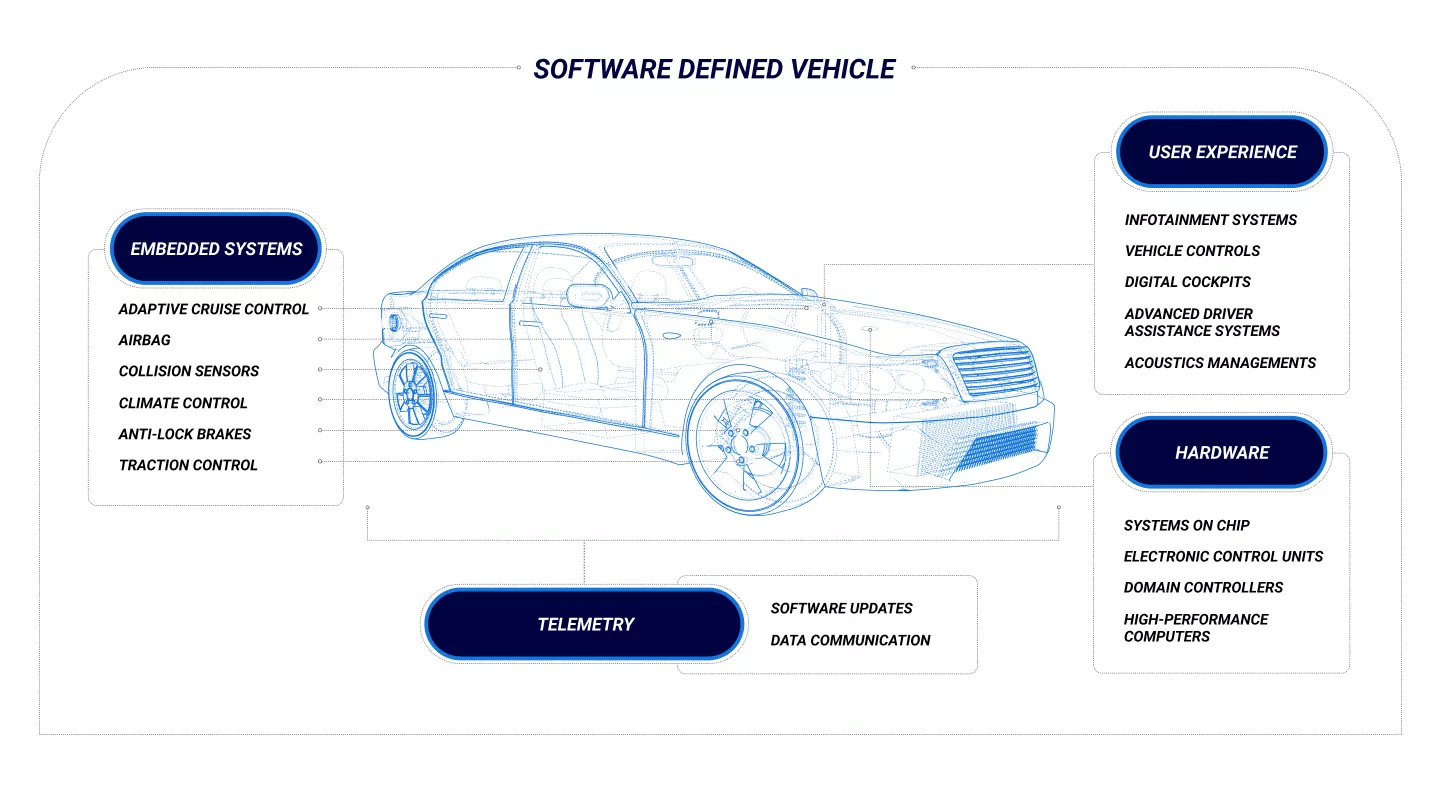
\includegraphics[scale=0.32]{Figures/Product/SDV.png}
  	\caption{Software defined vehicles}
  	\label{fig:Software defined vehicles}
\end{figure}

At its core, an SDV relies on software systems to control and manage various aspects of the vehicle's operations. These software systems govern functions such as engine management, powertrain control, braking, steering, and infotainment systems. By utilizing software, SDVs can offer improved performance, increased safety, and enhanced user experiences.

One of the key features of SDVs is their ability to collect and analyze vast amounts of data from various sensors and sources within the vehicle. This data includes information from cameras, radars, LiDARs, GPS, and other sensors, which is processed and utilized for various purposes such as object detection, collision avoidance, adaptive cruise control, and autonomous driving capabilities.

SDVs also leverage connectivity technologies to interact with the external environment. They can communicate with other vehicles, infrastructure systems, and cloud-based services to exchange information, access real-time data, and enhance driving experiences. Connectivity enables features like vehicle-to-vehicle (V2V) and vehicle-to-infrastructure (V2I) communication, enabling cooperative driving, traffic optimization, and enhanced safety.

Furthermore, SDVs often incorporate advanced software update mechanisms, allowing manufacturers to remotely deploy software updates and enhancements to vehicles. Over-the-air (OTA) updates eliminate the need for physical visits to service centers, providing convenience, efficiency, and the ability to continuously improve and upgrade vehicle functionalities.

The concept of SDVs also extends beyond individual vehicles. It encompasses the integration of vehicles into larger smart mobility ecosystems, where vehicles can communicate and collaborate with each other, infrastructure systems, and mobility service providers. This integration facilitates intelligent transportation systems, shared mobility, and the potential for more efficient and sustainable transportation solutions.

Overall, SDVs represent the convergence of software, connectivity, and advanced technologies in the automotive industry. By leveraging software-defined capabilities, these vehicles offer enhanced performance, safety, connectivity, and intelligent features, paving the way for the future of mobility.

\section{Importance of cloud development for creating SDVs}
Software-defined vehicles (SDVs) revolutionize the automotive industry by integrating cloud computing technologies into vehicle systems and operations. The cloud plays a pivotal role in enabling advanced functionalities, seamless connectivity, and scalable services for SDVs.

The cloud infrastructure provides a scalable and flexible platform for hosting the back-end services and data processing capabilities required by SDVs. It acts as a centralized hub that stores and processes massive amounts of data generated by vehicles, including sensor data, telemetry, navigation information, and multimedia content. This data is securely transmitted to the cloud, where it is analyzed, aggregated, and used to derive valuable insights for various purposes, such as optimizing vehicle performance, improving driving behaviors, and enhancing predictive maintenance.



SDVs leverage cloud-based analytics and machine learning algorithms to extract meaningful information from the collected data. These advanced analytics enable real-time monitoring of vehicle health, driver behavior analysis, and predictive maintenance. By analyzing historical data and patterns, the cloud can provide intelligent recommendations and insights to optimize driving efficiency, reduce fuel consumption, and enhance safety.

Moreover, the cloud enables seamless connectivity between vehicles and external entities. SDVs can communicate with cloud-based services and applications to access real-time traffic information, weather updates, navigation assistance, and personalized infotainment features. This connectivity enhances the driving experience, enabling drivers to stay connected, access relevant information, and leverage value-added services on the go.

In addition, the cloud plays a crucial role in delivering over-the-air software updates to SDVs. With a cloud-based software update management system, manufacturers can securely distribute and deploy software updates to vehicles remotely. This eliminates the need for physical recalls or service appointments, as updates can be seamlessly delivered to vehicles over the air. The cloud also enables efficient version control, rollback capabilities, and monitoring of the software update process, ensuring the integrity, security, and reliability of the updated software.

Cloud-based services and applications can also enhance vehicle-to-cloud and cloud-to-vehicle communication. SDVs can leverage cloud connectivity for advanced features like remote diagnostics, remote control, and fleet management. For example, fleet managers can monitor the performance and health of vehicles in real-time, optimize routes, allocate resources efficiently, and remotely configure vehicle settings.

Furthermore, the cloud enables data sharing and collaboration among SDVs, infrastructure systems, and other stakeholders. Vehicle-to-cloud communication allows SDVs to share valuable information with each other and with the cloud platform. This information sharing can contribute to collective intelligence, cooperative driving, and overall traffic optimization. For instance, vehicles can exchange data about road conditions, traffic congestion, and potential hazards, enabling other vehicles to make informed decisions and adapt their driving behavior accordingly.

In our project, we aim to explore and analyze the initiatives and advancements in the field of Software-Defined Vehicles (SDVs) from a market perspective. Our focus is on uncovering the latest developments, trends, and innovations in the realm of SDVs and understanding their impact on the automotive industry.

To achieve this, we will conduct comprehensive research to identify and examine the key players, companies, and organizations driving the SDV market. We will analyze their strategies, product offerings, and market positioning to gain insights into the competitive landscape and the direction in which the industry is heading.

Furthermore, we will dive into the latest architectures and technological frameworks that have emerged in the field of SDVs. This includes studying concepts such as cloud-based architectures, edge computing and connectivity protocols. We will investigate how these architectures are being implemented and their implications for the functionality, performance, and user experience of SDVs.

Additionally, our project will involve conducting market surveys, interviews, and case studies to gather firsthand information and perspectives from industry experts, automotive manufacturers, technology providers, and end-users. This primary research will provide valuable insights into market dynamics, consumer preferences, challenges, and opportunities related to SDVs.

Through our comprehensive analysis and research, we aim to contribute to the existing body of knowledge on SDVs and provide valuable insights for stakeholders in the automotive industry. By uncovering the latest initiatives, architectures, and market trends, our project will shed light on the future of SDVs and assist in shaping strategies for businesses, policymakers, and researchers in this dynamic and rapidly evolving field.

\section{Motivation}
The motivation behind undertaking a project focused on Software-Defined Vehicles (SDVs) stems from the profound impact that software and connectivity are having on the automotive industry. The convergence of software, artificial intelligence, and connectivity technologies is revolutionizing the way vehicles are designed, manufactured, operated, and experienced by users.

SDVs present a paradigm shift in the automotive landscape, offering numerous benefits such as enhanced safety, improved efficiency, increased functionality, and personalized user experiences. These vehicles leverage advanced software systems and algorithms to enable features like autonomous driving, real-time data analysis, predictive maintenance, and seamless integration with smart infrastructure.

By embarking on a project centered on SDVs, we aim to explore the transformative potential of these vehicles and their implications for various stakeholders, including manufacturers, consumers, and society as a whole. We are driven by the desire to understand the challenges, opportunities, and key considerations associated with the development and deployment of SDVs.

Furthermore, the project seeks to contribute to the growing body of knowledge in this field and foster innovation by studying the latest architectures, technologies, and market dynamics related to SDVs. By examining the market perspective, uncovering industry initiatives, and analyzing emerging trends, we aim to provide insights that can inform strategic decision-making, drive industry collaboration, and shape the future of the automotive sector.

Ultimately, our project aims to facilitate a deeper understanding of SDVs and their potential to revolutionize transportation. By shedding light on the transformative power of software-defined technologies in the automotive industry, we hope to inspire further research, development, and adoption of SDVs, ultimately leading to safer, more efficient, and sustainable mobility solutions for the future.
\section{Definition and purpose}
\subsection{Definition}
The graduation project aims to explore the potential of Software Defined Vehicles (SDVs) by integrating telematics control units with a cloud platform. It focuses on enabling vehicles to become software defined entities, allowing for standard, autonomous, and secure updates to the vehicle system. The project also involves developing a software update management system and implementing Vehicle-to-Vehicle (V2V) communication security using Vehicle-to-Infrastructure (V2I) technology. Additionally, the project focuses on creating an intuitive interface for vehicle owners to access and control their vehicles from smartphones, as well as introducing Vehicle-to-Cloud (V2C) features for enhanced connectivity and access to cloud-based services. The involvement of key industry players in SDVs further emphasizes the significance of this research in advancing the automotive industry.
\subsection{Purpose}
The purpose of this graduation project is to explore and advance the concept of Software Defined Vehicles (SDVs) by addressing key objectives. By integrating telematics control units with a cloud platform, the project aims to transform vehicles into software defined entities, allowing for efficient and secure updates to the vehicle system. The project also aims to enhance the security of V2V communication through the use of V2I technology, ensuring the authenticity of surrounding vehicles and promoting safe and reliable communication. Additionally, the project focuses on improving the user experience by developing an intuitive smartphone interface for vehicle owners to access and control their vehicles conveniently. Furthermore, the introduction of V2C features enables vehicles to connect and communicate with cloud-based services, expanding their functionality and providing access to a wide range of services and data. The findings and outcomes of this project contribute to the advancement of SDVs and provide valuable insights for further research and development in the field.
\section{Problem Statement}
\subsection{Safety and Security}
One of the key challenges in the development of Software-Defined Vehicles (SDVs) is ensuring the safety and security of the software and communication systems. As SDVs rely heavily on software algorithms, connectivity, and data exchange, vulnerabilities and potential cyber threats pose significant risks. The project aims to address the challenge of designing robust security measures, implementing secure communication protocols, and developing reliable fail-safe mechanisms to ensure the safety of SDVs and protect against potential cyberattacks.

\subsection{Standardization and Interoperability}
With the rapid evolution of SDV technologies, the lack of standardization and interoperability among different components and systems is a significant challenge. SDVs involve complex software architectures, multiple sensors, communication networks, and control systems, making it crucial to establish common standards and protocols for seamless integration and interoperability. The project focuses on exploring and developing standardized frameworks, protocols, and interfaces that enable interoperability between various SDV components, facilitating collaboration and compatibility among different manufacturers and service providers.
\subsection{Ethical and Legal Implications}
As SDVs become more advanced and autonomous, ethical and legal considerations arise. The project addresses questions related to liability, responsibility, and decision-making in critical situations. It explores the ethical implications of autonomous decision-making algorithms, such as how SDVs prioritize safety, handle potential accidents, and navigate complex moral dilemmas. Additionally, the project delves into the legal frameworks and regulatory requirements necessary to govern the deployment and operation of SDVs, ensuring compliance with local and international laws.

\subsection{User Acceptance and Trust}
The successful adoption of SDVs relies on user acceptance and trust in the technology. The project examines factors influencing user perception, concerns, and attitudes towards SDVs, including issues such as privacy, data collection, and the reliability of autonomous systems. It aims to identify strategies to increase user acceptance, improve transparency, and build trust by addressing user concerns through effective communication, education, and user-centered design principles.

\subsection{Infrastructure Readiness}
The deployment of SDVs requires a supportive infrastructure that includes robust communication networks, intelligent transportation systems, and infrastructure-to-vehicle connectivity. The project investigates the readiness of existing infrastructure to accommodate SDVs and identifies the necessary upgrades and investments needed to enable seamless integration and communication. It explores challenges related to network coverage, latency, data transmission, and infrastructure compatibility to ensure the infrastructure can support the demands of SDVs effectively.

\chapter{Literature Survey and Background}
\section{Brief history of Software defined vehicles}
The concept of software-defined vehicles (SDVs) has its roots in the evolution of automotive technology over the past few decades. The history of SDVs can be traced back to the advancements in electronic control systems and the increasing integration of software into vehicles.

In the 1980s, electronic control units (ECUs) started replacing mechanical and analog systems in vehicles. ECUs, which are essentially embedded systems, began controlling various functions such as engine management, braking systems, and airbags. This marked the beginning of the digitalization of automotive systems.

As the complexity of automotive systems increased, manufacturers started incorporating more software-based features and functionalities. In the late 1990s and early 2000s, vehicle systems like navigation, infotainment, and advanced driver-assistance systems (ADAS) became more prevalent. These systems relied heavily on software algorithms and required integration with sensors, processors, and communication networks.

The emergence of connected technologies and the Internet of Things (IoT) further paved the way for SDVs. The advent of reliable wireless communication protocols and the availability of high-speed mobile networks enabled vehicles to connect to the internet and access cloud-based services. This connectivity facilitated real-time data exchange, software updates, and remote diagnostics.

The introduction of electric vehicles (EVs) also played a significant role in the development of SDVs. EVs heavily rely on software for battery management, regenerative braking, energy efficiency optimization, and charging infrastructure integration. Software algorithms and control systems are crucial for the efficient operation and performance of electric powertrains.

In recent years, the automotive industry has witnessed significant advancements in autonomous driving technology. SDVs have become synonymous with self-driving cars, which leverage a multitude of sensors, cameras, radar, and lidar systems to perceive the environment and make autonomous driving decisions. The software stack that powers autonomous vehicles encompasses complex algorithms for perception, decision-making, and control.

The history of SDVs is characterized by the gradual integration of software and digital technologies into vehicles, leading to increased functionality, connectivity, and automation. This evolution has been driven by advancements in software engineering, communication technologies, and the demand for safer, more efficient, and connected transportation solutions. SDVs are poised to play a central role in shaping the future of mobility.

\section{Interested companies in SDV}
\subsection{Ford}
Ford has been actively exploring software-defined vehicles as part of their commitment to innovation and technology-driven mobility solutions. They have been investing in autonomous driving research and development, aiming to create self-driving vehicles that can navigate and operate safely in various environments. Ford's approach to SDVs involves leveraging advanced software algorithms, sensor technologies, and connectivity to enable intelligent and autonomous features in their vehicles.
\subsection{BMW}
BMW is another prominent player in the automotive industry that has shown a strong interest in software-defined vehicles. They have been focusing on developing intelligent, connected, and electric vehicles that offer a seamless integration of software and hardware. BMW's SDV initiatives revolve around creating a digital ecosystem that enables personalized and intuitive driving experiences. They aim to incorporate features such as advanced driver-assistance systems, intelligent connectivity, and over-the-air updates to enhance the performance, comfort, and sustainability of their vehicles.
\subsection{Toyota}
Toyota has been actively involved in exploring and implementing software-defined vehicle technologies. They recognize the importance of software in enabling advanced features, connectivity, and autonomous capabilities in vehicles. Toyota's approach to SDVs involves integrating software-driven functionalities, such as advanced driver-assistance systems and connected services, to enhance safety and convenience for their customers. They also emphasize the importance of collaboration and partnerships to drive innovation and accelerate the development of SDV technologies.
\subsection{Volkswagen}
The Volkswagen Group has been actively pursuing software-defined vehicle initiatives as part of their strategic vision for future mobility. They are investing in software platforms and architectures that enable seamless integration of software components and systems within their vehicles. Volkswagen aims to leverage software-defined features, including autonomous driving capabilities, intelligent infotainment systems, and connected services, to deliver enhanced driving experiences and sustainable mobility solutions.
\subsection{NVIDIA}
While not a traditional automotive manufacturer, NVIDIA is a technology company that plays a significant role in enabling software-defined vehicles. They provide advanced hardware and software solutions, including powerful GPUs and AI computing platforms, that are used by automakers and autonomous driving technology developers. NVIDIA's expertise lies in developing high-performance computing solutions that can handle the computational demands of AI-driven systems, making them a key player in the development of software-defined vehicles.
\subsection{Tesla}
Tesla is one of the leading companies that has shown a significant interest in software-defined vehicles (SDVs). Known for their electric vehicles and advanced autonomous driving features, Tesla has been at the forefront of innovation in the automotive industry. They heavily rely on software and over-the-air updates to enhance and add new functionalities to their vehicles. Tesla's approach to SDVs involves continuous improvement and feature expansion through software updates, allowing their vehicles to evolve and adapt to changing user needs.

These companies, along with several others, demonstrate a strong interest and commitment to software-defined vehicles. Through their investments in research, development, and strategic partnerships, they are shaping the future of mobility by harnessing the power of software and advanced technologies to deliver innovative, connected, and autonomous driving experiences.
\newpage
\section{Initiatives and alliances that work in SDV}
There are several initiatives and alliances that work in the field of software-defined vehicles (SDVs) to drive innovation, collaboration, and standardization. These organizations aim to accelerate the development and deployment of SDV technologies. Some notable initiatives and alliances include:
\subsection{Esync alliance}
The eSync Alliance \cite{eSyncAlliance} is an industry consortium that focuses on establishing and promoting standards for over-the-air (OTA) updates and data exchange in connected vehicles. The alliance aims to simplify and streamline the process of delivering software updates and data to vehicles, ensuring secure and efficient communication between the cloud, backend systems, and the vehicle's electronic systems.

The eSync Alliance brings together a diverse group of companies, including automakers, Tier 1 suppliers, software providers, and semiconductor manufacturers. By collaborating and sharing expertise, the alliance works towards creating a common platform that enables seamless and secure OTA updates, diagnostics, and data management for connected vehicles.

One of the primary objectives of the eSync Alliance is to develop and maintain specifications and protocols that define the communication and interoperability standards between various components of the automotive ecosystem. This includes defining standards for data formats, message exchange protocols, security mechanisms, and device management frameworks.

The alliance's focus on standardization helps overcome the challenges associated with the growing complexity of automotive software and the need for frequent updates and enhancements. By establishing common standards, the eSync Alliance aims to reduce development costs, improve efficiency, and ensure compatibility across different vehicle platforms.

Moreover, the eSync Alliance promotes collaboration and knowledge sharing among its members through working groups, workshops, and industry events. Members have the opportunity to contribute to the development of specifications, influence the direction of OTA update technologies, and share best practices.

Overall, the eSync Alliance plays a crucial role in driving the adoption and implementation of OTA update and data exchange technologies in the automotive industry. By establishing standards and fostering collaboration, the alliance aims to accelerate the deployment of connected vehicles with robust and efficient software update capabilities, enhancing the overall user experience, safety, and functionality of modern vehicles.

\subsection{Covesa Initiative}
The CoVeSA (Connected Vehicle Services Architecture) \cite{CovesaAlliance} initiative is a collaborative effort aimed at developing a standardized architecture for connected vehicle services. CoVeSA brings together various stakeholders in the automotive industry, including automakers, suppliers, and technology providers, to define a common framework for delivering connected services in vehicles.

The initiative recognizes the increasing importance of connectivity and digital services in modern vehicles. It aims to address the challenges associated with developing and deploying connected vehicle services by providing a standardized architecture that promotes interoperability, scalability, and security.

CoVeSA focuses on defining a modular architecture that allows for the integration of various services, such as infotainment, navigation, telematics, and remote diagnostics, into the vehicle's ecosystem. The architecture provides a set of standardized interfaces, protocols, and data models that enable seamless communication and data exchange between different components and systems within the vehicle.

By establishing a common architecture, the CoVeSA initiative aims to simplify the development and deployment of connected vehicle services. It enables automakers and suppliers to build and integrate services more efficiently, reducing development costs and time to market. Additionally, the standardized architecture facilitates collaboration and innovation by allowing third-party developers to create compatible applications and services for connected vehicles.

The CoVeSA initiative also emphasizes security and privacy considerations. It defines guidelines and best practices for securing the communication and data exchange between the vehicle and external systems, ensuring the protection of sensitive information and preventing unauthorized access.

Through collaborative working groups and regular meetings, the CoVeSA initiative enables its members to contribute to the development and refinement of the architecture. It provides a platform for sharing knowledge, exchanging ideas, and addressing common challenges in the connected vehicle services domain.
\newpage
\section{Known proposed architectures}
\subsection{SOAFEE architicture}
The Scalable Open Architecture for Embedded Edge (SOAFEE)\cite{SOAFEE_ARCH} project is an industry-led collaboration defined by automakers, semiconductor suppliers, open source and independent software vendors, and cloud technology leaders. The initiative intends to deliver a cloud-native architecture enhanced for mixed-criticality automotive applications with corresponding open-source reference implementations to enable commercial and non-commercial offerings.

\begin{figure}[!ht]
	\centering
	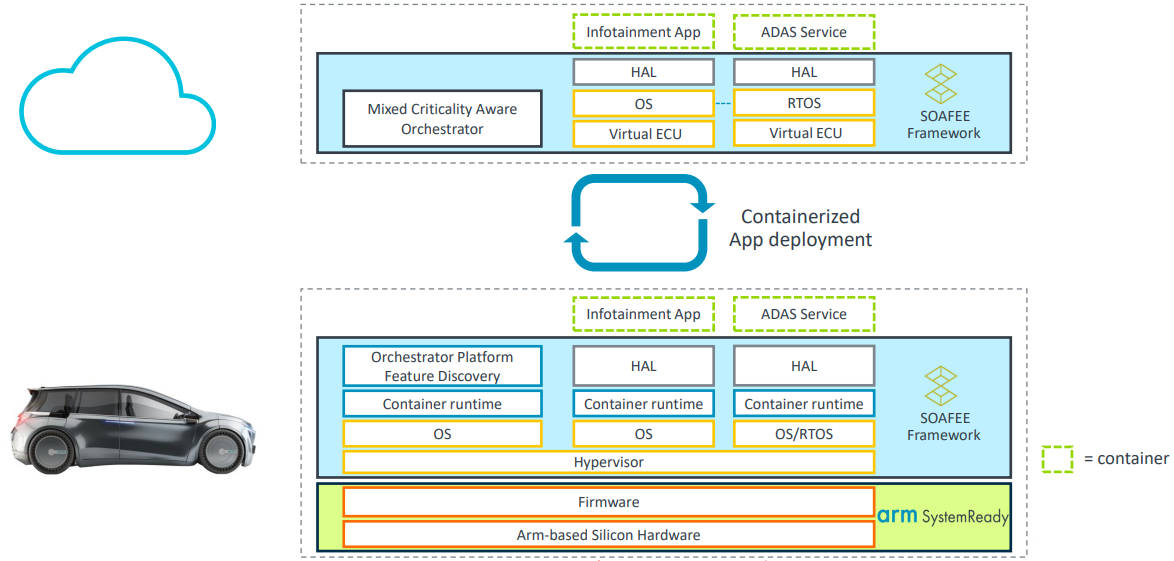
\includegraphics[scale=1.5]{Figures/Architicture/SOAPHEE.jpg}
  	\caption{SOAFEE specification}
  	\label{fig:SOAFEE specification}
\end{figure}

Building on technologies like Project Cassini and SystemReady, which define standard boot and security requirements for Arm architecture, SOAFEE adds the cloud-native development and deployment framework while introducing functional safety, security, and real-time capabilities required for automotive workloads.

\newpage
\subsection{AWS CAEdge architicture}

The AWS CAEdge architecture \cite{AWS_CAedge} is designed as a secure and scalable multi-tenant platform for software-intensive, vehicle-related workloads. The framework is based on modular building blocks, including the Scalable Compute Platform, Cloud services, and the DevOps Workbench. Each building block provides specific functionalities and APIs, allowing for easy integration and customization for various use cases.


\begin{figure}[!ht]
	\centering
	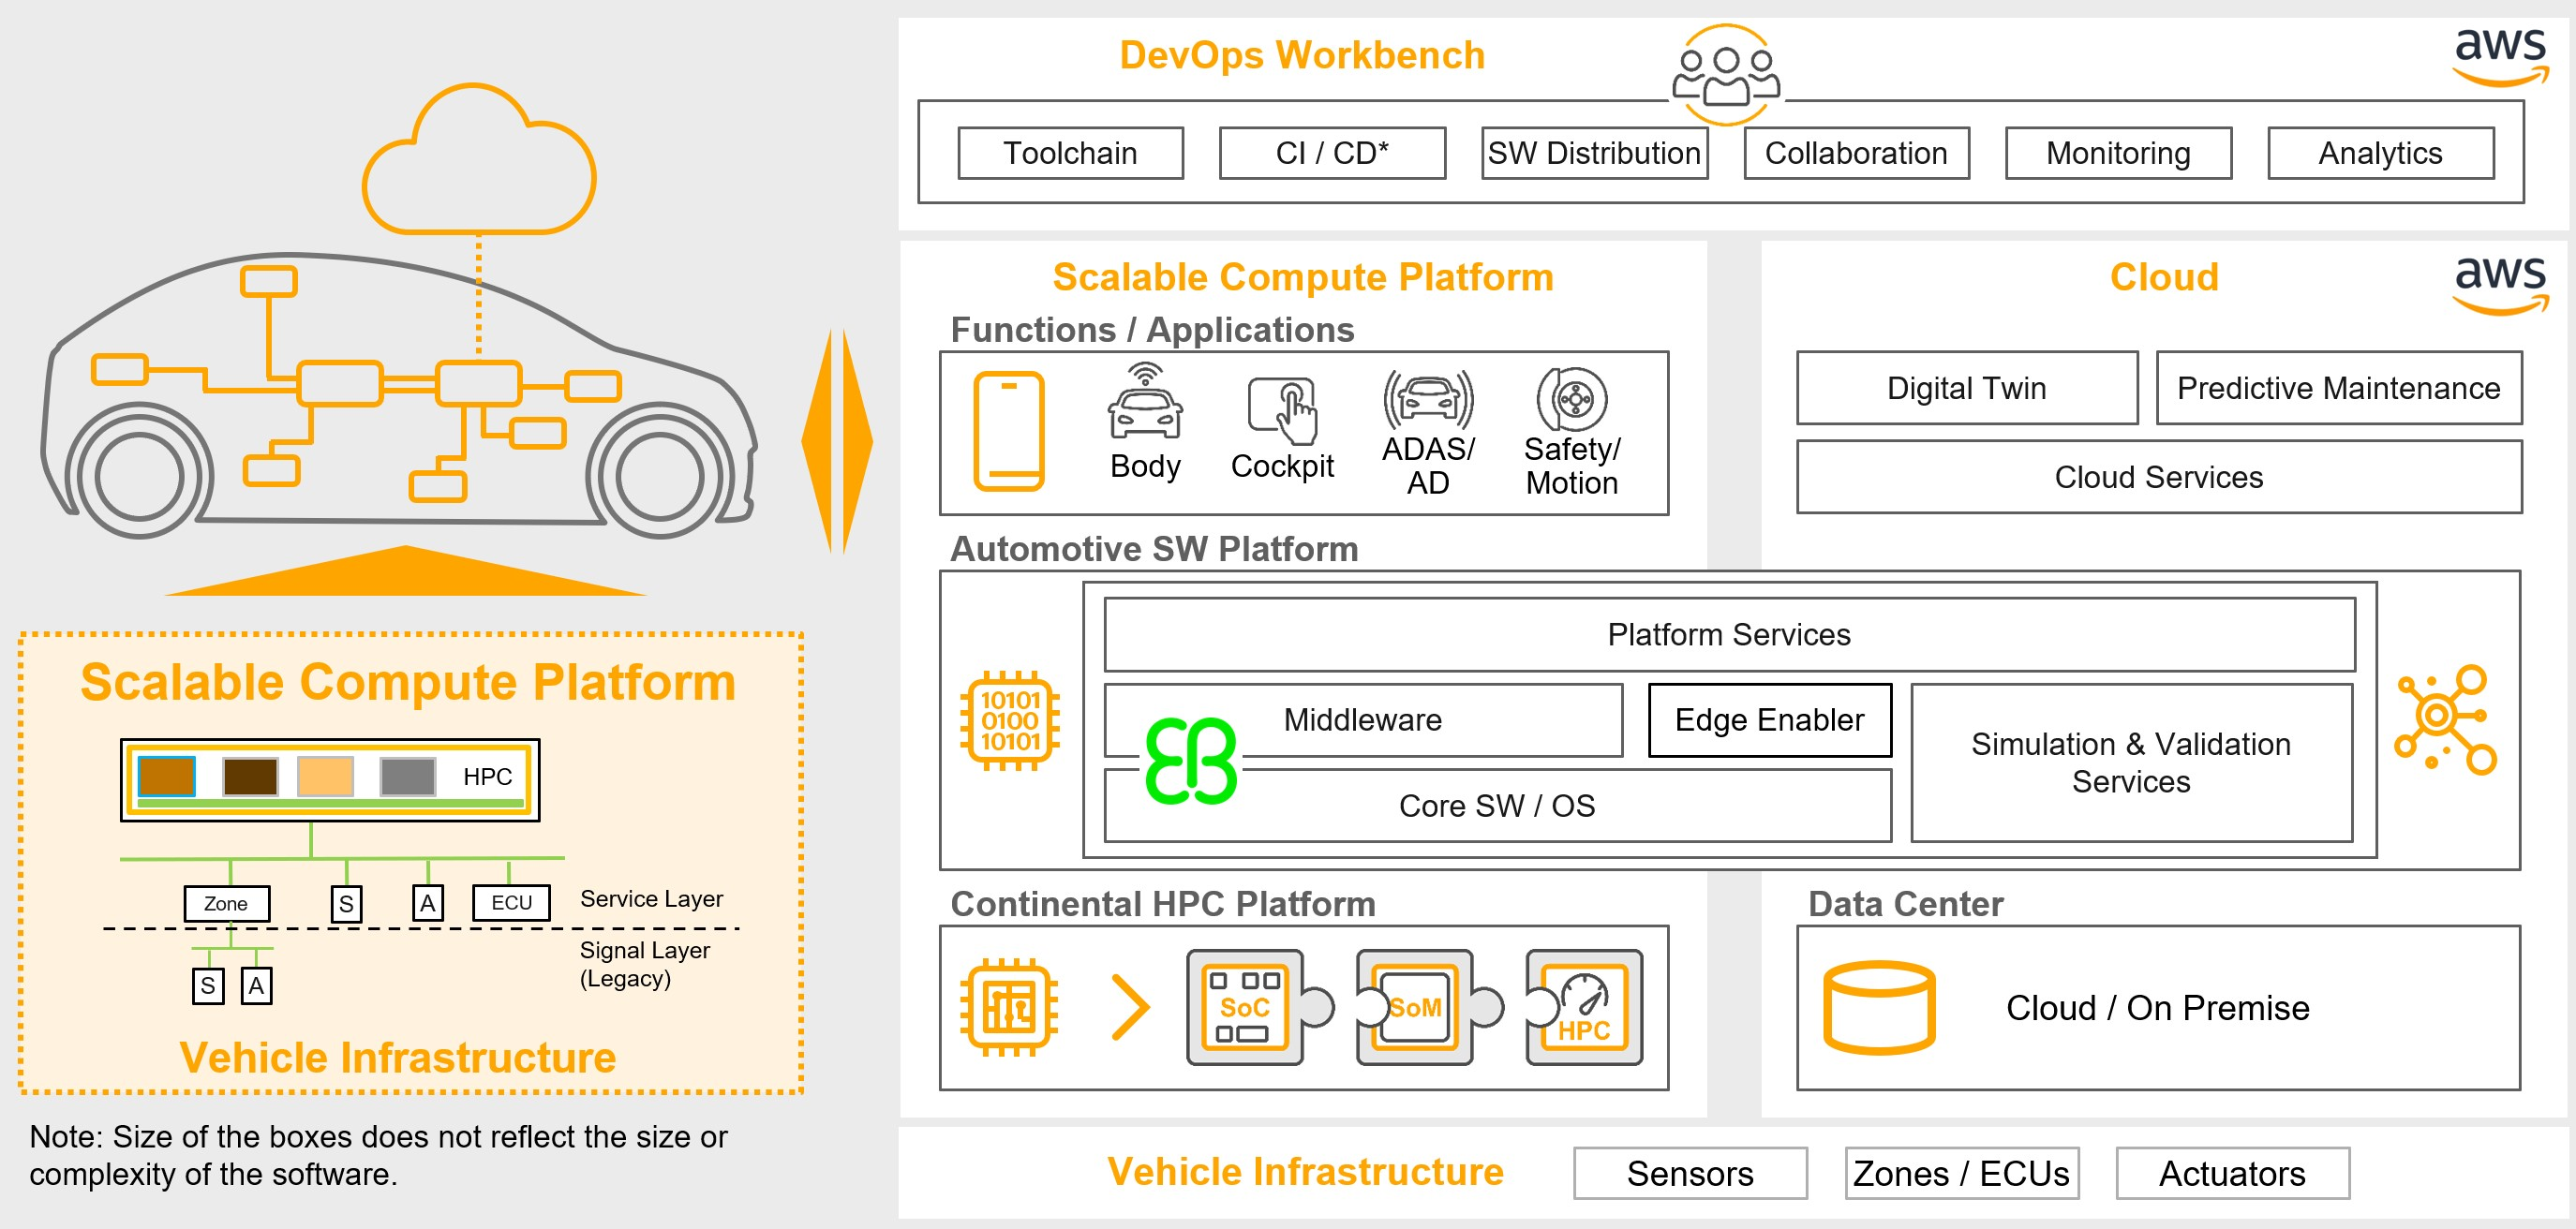
\includegraphics[scale=0.2]{Figures/Architicture/SDV_Cloud.jpg}
  	\caption{AWS CAEdge specification}
  	\label{fig:AWS CAEdge specification}
\end{figure}

The core architecture of the CAEdge framework is based on clear API operations and a tenant-aware approach. It operates within a dedicated AWS Organization, ensuring separation and isolation from other workloads. The framework employs a multi-layered security approach to achieve tenant separation and isolation. This includes using individual AWS Accounts for each tenant, assigning dedicated organizational units (OUs) with custom security policies, and leveraging a central metadata layer for automated IAM assignments and access management.

The architecture also emphasizes automation and self-service capabilities. Services like AWS Control Tower, AWS Deployment Framework (ADF), AWS Single Sign-On (SSO), and AWS DynamoDB are utilized to automate the creation and management of tenant-owned resources, projects, and workbenches. This high degree of automation enables rapid provisioning of developer workbenches within a tenant context, reducing setup time from weeks to minutes.

By adopting the AWS CAEdge architecture, Continental has established a secure and scalable platform that enables OEMs, suppliers, and partners to quickly onboard and start developing software-intensive solutions for vehicles. This solution accelerates the transformation into a software-centric organization, allowing developers to focus on building innovative solutions within hours instead of months.

\section{Used standards}

\subsection{UN R155}
UN Regulation No. 155, titled "Cyber Security and Cybersecurity Management," \cite{UNR155} is an important regulatory framework established by the United Nations Economic Commission for Europe (UNECE) to address the growing concern of cybersecurity in the automotive industry. The regulation aims to ensure the safe and secure operation of vehicles, focusing on the prevention and mitigation of cyber threats.

UN R155 provides a comprehensive set of guidelines and requirements for vehicle manufacturers, covering various aspects of cybersecurity. It emphasizes the need for robust cybersecurity measures throughout the vehicle's lifecycle, including the development, production, and maintenance stages. The regulation encourages the implementation of cybersecurity management systems that encompass risk assessment, threat analysis, incident response, and ongoing monitoring.

One of the key objectives of UN R155 is to enhance the resilience of vehicles against cyber attacks. It emphasizes the importance of secure vehicle communication systems, safeguarding the integrity and confidentiality of data exchanged between vehicles and external entities. The regulation promotes the use of secure communication protocols, encryption mechanisms, and authentication techniques to prevent unauthorized access and data manipulation.

Furthermore, UN R155 highlights the significance of software update processes and management systems. It addresses the need for secure and reliable software updates to ensure the continuous protection of vehicles against emerging cyber threats. The regulation emphasizes the importance of implementing effective update mechanisms, secure delivery channels, and validation procedures to maintain the integrity and authenticity of software updates.

In addition to technical requirements, UN R155 also emphasizes the importance of collaboration and information sharing among relevant stakeholders. It encourages cooperation between vehicle manufacturers, regulatory authorities, and cybersecurity experts to exchange best practices, share information about potential threats, and foster a proactive approach to cybersecurity in the automotive industry.

Overall, UN Regulation No. 155 plays a crucial role in promoting cybersecurity and establishing a common framework for ensuring the safe and secure operation of vehicles. By addressing key cybersecurity concerns and providing guidelines for implementation, the regulation aims to enhance consumer trust, protect user privacy, and mitigate the risks associated with cyber threats in the automotive ecosystem.
\subsection{UN R156}
UN Regulation No. 156, titled "Software Update Processes and Management Systems," \cite{UNR156} is an essential regulatory framework established by the United Nations Economic Commission for Europe (UNECE) to address the challenges and best practices associated with software updates in the automotive industry. The regulation aims to ensure the efficient and secure management of software updates throughout a vehicle's lifecycle.

UN R156 provides detailed guidelines and requirements for vehicle manufacturers regarding the implementation of effective software update processes and management systems. The regulation emphasizes the need for reliable and secure mechanisms to deliver software updates to vehicles, ensuring that updates are timely, accurate, and free from vulnerabilities.

One of the primary objectives of UN R156 is to ensure the integrity and authenticity of software updates. The regulation outlines the importance of using digital signatures and secure communication protocols to verify the source and integrity of software updates. By employing cryptographic techniques, such as digital certificates and secure communication channels, the regulation aims to prevent unauthorized modifications to software during the update process.

UN R156 also emphasizes the significance of over-the-air (OTA) updates, which allow for remote software updates without the need for physical intervention. The regulation sets requirements for OTA update processes, including secure communication channels, strong authentication mechanisms, and secure storage of update packages. These requirements aim to ensure the reliability, security, and privacy of OTA updates, enabling vehicle manufacturers to provide timely bug fixes, feature enhancements, and security patches to vehicles in a convenient and efficient manner.

Furthermore, the regulation highlights the importance of transparency and communication with end-users regarding software updates. It encourages vehicle manufacturers to provide clear information to consumers about the purpose, content, and potential impacts of software updates. This includes informing users about any changes in vehicle functionality, data collection practices, and privacy-related aspects that may result from the software update.

UN R156 also promotes collaboration and information sharing among stakeholders. It encourages the establishment of industry standards, best practices, and cooperation between vehicle manufacturers, regulatory authorities, and cybersecurity experts to ensure the continuous improvement of software update processes and management systems.

Overall, UN Regulation No. 156 addresses the critical aspects of software update management in the automotive industry. By setting guidelines and requirements for secure and efficient software updates, the regulation aims to enhance vehicle performance, functionality, and security while ensuring the safety and satisfaction of end-users.
\chapter{Solution Architecture}

\section{Architecture overview}
The system architecture is made up of four and five components, each of which is implemented as an interactive micro-service and works together to integrate a cloud server with a Telematics Control Unit (TCU) to create a software-defined vehicle. These elements include:


\begin{figure}[!ht]
	\centering
	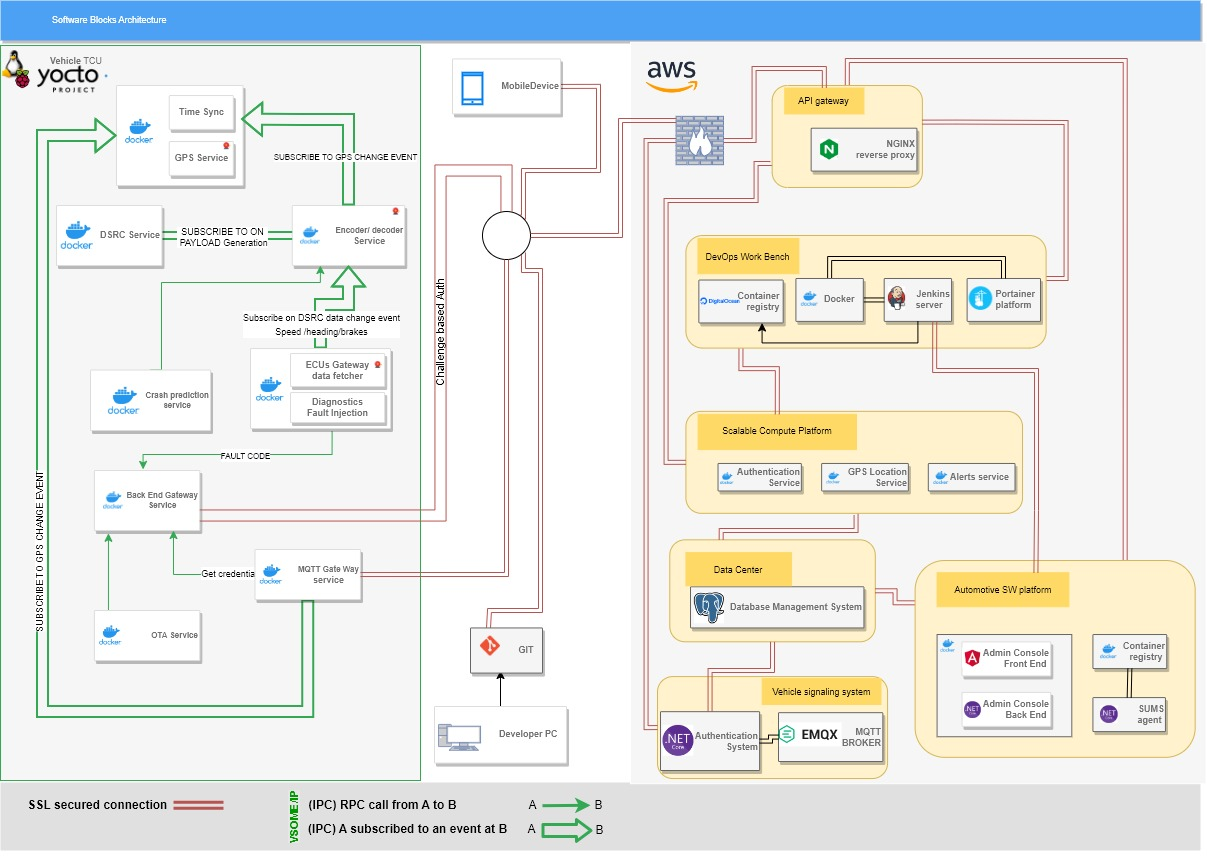
\includegraphics[scale=0.4]{Figures/Architicture/overview.jpg}
  	\caption{System architecture}
  	\label{fig:System architecture}
\end{figure}
\newpage
\subsection{Database Center}
This system serves as the storage backbone for all relevant data. It securely stores and manages vehicle-related information, user profiles, configuration settings, and other necessary data. By employing a robust database system, we ensure efficient and reliable data retrieval and storage for the entire system.

\subsection{Scalable Compute platform}
These services provide users with access to automotive features and functionalities through the cloud. By utilizing the cloud infrastructure, users can remotely interact with their vehicles, GPS tracking, receiving alerts, feature manipulation and retrieving vehicle diagnostics. The Cloud Back-end Services also facilitate seamless communication and interaction between the Telematics Control Unit and the cloud server.

\subsection{Vehicle signaling system}
The Vehicle signaling system enables efficient and lightweight communication between the server and the vehicle. This publish-subscribe messaging protocol allows the server to send commands, notifications, and updates to the TCU, which then executes the necessary actions in the vehicle. The Vehicle signaling system ensures reliable and real-time communication, enabling smooth and responsive control over the software-defined vehicle.

\subsection{Automotive SW platform}
This system handles over-the-air updates and manages the manipulation of vehicle features. It allows for seamless software updates to be delivered to the vehicle, ensuring that the software-defined functionalities remain up to date. Additionally, the system enables the addition of new features in the future, enhancing the capabilities and versatility of the software-defined vehicle.
\newpage
\subsection{DevOps Work Bench}
The system we have developed plays a crucial role in automating, monitoring, and maintaining our entire cloud infrastructure. It serves as a centralized platform responsible for continuous integration and continuous deployment (CI/CD) of the entire system, ensuring efficient and seamless software development processes.

The CI/CD aspect of the system enables automated build, testing, and deployment of software updates, ensuring the timely delivery of new features and bug fixes. It streamlines the development workflow, reducing manual efforts and minimizing the risk of human errors. Through automated testing and deployment pipelines, the system ensures the stability and reliability of the deployed software, enhancing overall system performance.

In addition to CI/CD, our system provides comprehensive monitoring capabilities for all the components within our cloud infrastructure. It collects and analyzes various performance metrics, such as CPU usage, memory utilization, network traffic, and response times, providing real-time insights into the system's health and performance. This monitoring functionality enables proactive identification of potential bottlenecks, performance issues, or anomalies, allowing for timely interventions and optimization.

Moreover, the system incorporates robust maintenance features to ensure the smooth operation of the cloud infrastructure. It includes automated backup and recovery mechanisms, periodic system updates, and proactive maintenance tasks. These measures help mitigate the risk of system failures, data loss, and security breaches, ensuring the availability and reliability of our services.

In the event of a system failure or crisis situation, our system is equipped with crisis management protocols. It includes predefined procedures and automated responses to handle critical incidents, such as infrastructure outages, security breaches, or performance degradation. These protocols help minimize downtime, restore services promptly, and mitigate the impact on users and operations.
By incorporating these five interconnected systems, our architecture provides a comprehensive solution for creating a software-defined vehicle. It ensures secure data storage, remote access to vehicle features, efficient communication between the server and the TCU, and seamless software updates and feature enhancements. The modular and scalable nature of the architecture allows for flexibility and adaptability to future advancements and user requirements.
\newpage
\section{Architectural style}
The foundation of our system architecture is built upon a micro-service-based approach, which offers numerous advantages for the development and operation of our software-defined vehicle solution. By decomposing the system into smaller, autonomous services, we have achieved greater flexibility, scalability, and maintainability. Each micro-service is responsible for a specific business capability or feature, allowing us to develop, deploy, and update individual services independently without affecting the entire system. This modular nature not only simplifies the development process but also enables us to scale the system horizontally by replicating or adding instances of specific micro-services as per demand. Additionally, the loose coupling between micro-services facilitates fault isolation, meaning that failures in one service do not cascade to others, resulting in increased resilience and system availability.

Micro-services exhibit a range of distinctive characteristics that contribute to their effectiveness in modern software architecture. One key characteristic is their autonomy, whereby each individual component operates independently and can be developed, deployed, operated, and scaled without impacting the functionality of other services. This level of autonomy enables teams to work on specific services without worrying about the intricate dependencies of the entire system. Communication between micro-services is facilitated through well-defined APIs, ensuring loose coupling and promoting flexibility. This decoupled nature allows for more efficient development, deployment, and evolution of individual services, as they can be modified or replaced without affecting the overall system.


\begin{figure}[!ht]
	\centering
	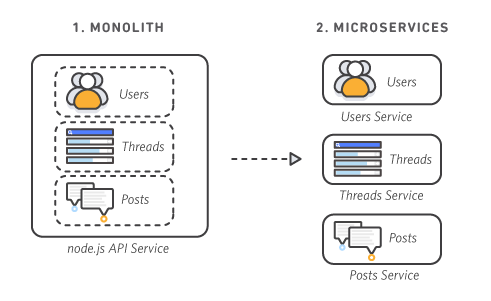
\includegraphics[scale=0.5]{Figures/Architicture/micro-services.png}
  	\caption{Microservices vs Monolothic development}
  	\label{fig:Microservices vs Monolothic development}
\end{figure}

Another essential characteristic of micro services is their specialization. Each service is designed to address a specific problem or provide particular capabilities. This specialization enables services to focus on a specific area of functionality, allowing for more modular and granular software development. As services evolve, they can be broken down into smaller, more specialized services, ensuring maintainability, scalability, and flexibility. The ability to decompose services into smaller, well-defined units enhances the overall agility of the system and enables independent development and deployment of specific functionalities. By having smaller and more focused services, teams can better understand and manage the complexity of individual components, leading to improved overall system maintainability and extensibility.

These characteristics of micro-services bring numerous benefits to software development and deployment. The autonomy of micro-services fosters agility within an organization, empowering small, independent teams to take ownership of their services. Teams can work autonomously and quickly, resulting in shorter development cycles and increased productivity. The specialized nature of micro-services also allows for flexible scaling, as each service can be independently scaled to meet the demand for its specific functionality. This fine-grained scaling ensures optimal resource utilization and responsiveness to varying workloads.

Furthermore, the autonomy and specialization of micro-services contribute to easy deployment through continuous integration and continuous delivery practices. Each micro-service can be developed, tested, and deployed independently, enabling rapid experimentation, validation of ideas, and quick iteration cycles. This decoupled deployment approach also simplifies rollbacks in case of issues or failures, minimizing downtime and ensuring a more stable and reliable system.

Moreover, the modular and independent nature of micro-services promotes technological freedom. Teams have the flexibility to choose the best tools, technologies, and frameworks for each micro-service based on its specific requirements. This freedom allows for the selection of optimal solutions for individual services, taking advantage of the latest advancements and adapting to evolving needs.

Additionally, micro-services encourage code reuse by dividing software into small, well-defined modules. Functionalities implemented in one micro-service can be leveraged as building blocks for other services, reducing duplication of effort and enhancing development efficiency. This code reuse contributes to faster development cycles and more streamlined maintenance.

Lastly, the autonomy and fault isolation provided by micro-services enhance the resilience of the overall system. If a single micro-service fails, the impact is limited to that specific service, preventing the entire system from collapsing. The fault isolation ensures that failures are contained, allowing the system to gracefully degrade functionality while maintaining overall stability and availability.

In summary, the autonomous and specialized nature of micro-services, along with their associated benefits of agility, flexible scaling, easy deployment, technological freedom, code reuse, and resilience, make them a powerful architectural approach for developing complex software systems. These characteristics empower teams to work independently, optimize resources, quickly adapt to changing requirements, and build robust and scalable applications.
\section{Architecture components}
\subsection{Scalable Compute platform}
Our cloud back-end services play a pivotal role in enabling the functionality and seamless integration of features within our Software Defined Vehicle (SDV) system. Serving as the backbone of our SDV, these services provide the necessary APIs for every automotive feature that requires cloud functionalities. This integration ensures that every interaction the user has with their vehicle is facilitated through our cloud server, which acts as a hidden layer between the user and their automotive.

The cloud backend system comprises a collection of independent sand-boxed environments, each hosting a specific feature. This modular approach allows for the isolation and secure execution of each feature within its own environment while enabling seamless interaction and communication with other components of the system. This design ensures the scalability, maintainability, and fault tolerance of our cloud back-end services.

Throughout the course of our project, we have successfully developed and implemented multiple features within our cloud back-end system. These features encompass a diverse range of functionalities that enhance the user experience and provide valuable services. In the following sections, we will provide comprehensive details and explanations for each of these features.

\subsubsection{Location live tracking}
One of the prominent features offered by our cloud backend services is live location tracking of the user's vehicle. This feature allows users to track their vehicle's real-time location upon request. The process involves the establishment of a persistent connection between the user and the feature hosting server, enabling seamless communication throughout the tracking session.

When a user initiates the live location tracking service, they create a persistent connection with the feature hosting server. Through this connection, the user invokes the GPS tracking service, indicating their intent to monitor the vehicle's location. The GPS server validates the user's authority to access the location information for the specified vehicle.

Upon successful authorization, the GPS server interacts with the MQTT system to send a signal to the automotive, requesting the sharing of its live location data. The MQTT system serves as a reliable and efficient messaging protocol for server-to-vehicle signaling. The automotive receives the signal and begins transmitting its real-time coordinates to the server.

Meanwhile, the hosting server, using the persistent connection established with the user, forwards the received coordinates from the automotive. The server continuously updates the user with the vehicle's current location using the same persistent connection until the user decides to terminate the tracking session.

When the user terminates the connection or requests to stop sharing the location, a signal is sent to the automotive through the MQTT system, instructing it to cease transmitting the location data. This ensures that the vehicle's live location sharing is halted, and the user's privacy is protected.

The implementation of this feature involves careful coordination between the GPS server, MQTT system, and the auto-motive's capabilities. It leverages the persistent connection to maintain a seamless flow of location data from the automotive to the user, allowing them to track their vehicle's movements in real-time.

By offering live location tracking as part of our cloud back end services, we provide users with an essential capability to monitor their vehicles' whereabouts. This feature enhances safety, security, and convenience for users, enabling them to have better control and awareness of their automotive assets.

\subsubsection{notifications and alerts}
In our SDV system, we have developed a comprehensive platform that enables automotive vehicles to send timely and important notifications to their owners. This feature serves as a crucial communication channel between the vehicle's Telematics Control Unit (TCU) and the server, ensuring that owners are promptly notified of any significant events or malfunctions occurring within their automotive.

When an event or malfunction occurs in the vehicle, the TCU initiates a request to the server. This request contains essential information about the event, such as the type of malfunction and its severity. To facilitate the seamless delivery of notifications, we leverage the power of the Fire-base Cloud Messaging (FCM) protocol.

Using the FCM protocol, the server interacts with the FCM infrastructure to send notifications directly to the vehicle owners' devices. FCM provides a reliable and efficient messaging service, ensuring that notifications are delivered in real-time to the intended recipients. This enables owners to stay informed about the status of their automotive and take appropriate actions promptly.

The FCM integration allows us to leverage the advanced capabilities provided by the protocol. For instance, we can personalize the notifications, include relevant details about the malfunction, and tailor the message content to provide clear instructions or recommendations to the owners. Furthermore, FCM supports rich media and deep linking, enabling us to enhance the notifications with additional information or interactive elements, creating a more engaging user experience.

To ensure a secure and reliable communication channel, the FCM protocol employs industry-standard encryption and authentication mechanisms. This protects the privacy and integrity of the notifications being transmitted between the server and the owners' devices. By leveraging FCM, we guarantee that the notification delivery process is robust, efficient, and adheres to the highest security standards.

Through this feature, automotive owners can receive notifications promptly and effectively, keeping them informed about any malfunctions or important events happening within their vehicles. This not only enhances their overall ownership experience but also enables them to take timely actions, such as scheduling maintenance or seeking assistance, to ensure the proper functioning and safety of their automotive.

In summary, our platform leverages the power of the Fire-base Cloud Messaging protocol to enable automotive vehicles to send notifications to their owners. By integrating FCM, we ensure the reliable and secure delivery of real-time notifications, providing owners with crucial information about malfunctions or significant events. This feature enhances the user experience and empowers automotive owners to stay connected with their vehicles, fostering a sense of control, safety, and peace of mind.

\subsubsection{Authentication system}
In order to ensure the overall security of our system modules, we have implemented advanced authentication and authorization schemes. These schemes are designed to protect both user data and the data shared by the automotive itself, thereby establishing a secure environment for our SDV platform. 

To achieve this, our authentication scheme has been divided into two distinct domains: the mobile device domain and the TCU domain. 

In the mobile device domain, we have implemented robust authentication mechanisms to secure user data and access to the SDV platform. This includes user authentication protocols such as username/password combinations, biometric authentication (such as fingerprint or facial recognition), and two-factor authentication for an added layer of security. These authentication methods ensure that only authorized users can access the system and their associated data.

On the other hand, in the TCU domain, we have implemented authentication measures to secure the communication and data exchange between the automotive and the server. The Telematics Control Unit (TCU) plays a crucial role in connecting the vehicle to our platform. To ensure secure communication, we employ industry-standard protocols such as mutual authentication, where both the server and the TCU authenticate each other to establish a secure and trusted connection. This authentication process helps prevent unauthorized access to the TCU and protects the integrity and confidentiality of the data transmitted between the automotive and the server.

Furthermore, our authorization schemes go hand in hand with the authentication mechanisms. Once users and TCUs are successfully authenticated, they are granted access to specific functionalities and resources based on predefined roles and permissions. This ensures that only authorized entities can perform certain actions within the system and access sensitive information.

By implementing these advanced authentication and authorization schemes, we have created a secure foundation for our SDV platform. These measures protect user data, prevent unauthorized access, and maintain the confidentiality and integrity of the shared automotive data. We continually monitor and update our security protocols to stay ahead of emerging threats and ensure the ongoing protection of our system and users' information.

In summary, the implementation of advanced authentication and authorization schemes in both the mobile device and TCU domains strengthens the security of our system modules. These measures safeguard user data and establish secure communication channels between the users, the automotive, and the server. By adhering to industry-standard security practices, we provide users with a trusted and secure environment to interact with our SDV platform, fostering confidence in the confidentiality and integrity of their data.

\subsection{Vehicle signaling system}
In the dynamic environment of automotive systems, characterized by high mobility and constantly changing logical addresses of vehicles, the traditional client/server model becomes impractical and ineffective. The client/server model relies on the concept of sending requests to specific logical addresses and expecting responses. However, in the automotive context, it is not feasible to identify and maintain the logical address of a vehicle due to its continuous movement and changing network configurations.

To address this challenge, we needed to devise an innovative solution that could enable seamless and efficient communication between vehicles and the backend services. This led us to explore the concepts of Software-Defined Networks (SDNs) and the MQTT protocol.

SDNs offer a paradigm shift in network architecture, providing a centralized control plane that can dynamically manage and control network resources. By decoupling the control plane from the data plane, SDNs allow for the programmability and flexibility needed to adapt to the dynamic nature of automotive environments. In our solution, we leveraged SDNs to create a network infrastructure that could accommodate the mobility and changing logical addresses of vehicles.

MQTT, with its publish-subscribe messaging pattern and lightweight nature, emerged as a suitable protocol for communication in this context. Unlike the client/server model, MQTT enables devices (in this case, vehicles) to publish messages to specific topics and subscribe to topics of interest without the need for knowing the exact logical addresses of the recipients. The MQTT broker acts as a centralized intermediary that routes messages to the appropriate subscribers based on their topic subscriptions. This approach aligns well with the dynamic nature of automotive environments, where vehicles can publish updates or request specific services without the need for direct knowledge of the recipients.

By combining the principles of SDNs and the MQTT protocol, we created a more innovative solution that allows vehicles to communicate effectively with back-end services in a dynamic and mobile environment. The SDN infrastructure provides the necessary control and adaptability, while MQTT facilitates efficient message exchange based on topic subscriptions, eliminating the need for static logical addresses. This approach enables seamless and flexible communication between vehicles and the back-end services, ensuring the delivery of critical information, real-time updates, and service requests.

Overall, our innovative approach of integrating SDNs and MQTT addresses the limitations of the traditional client/server model in the automotive context. It leverages the dynamic capabilities of SDNs to accommodate vehicle mobility and utilizes the publish-subscribe model of MQTT to enable efficient and effective communication without relying on static logical addresses. This combination allows for scalable, flexible, and reliable communication in automotive systems, enhancing the overall functionality and responsiveness of the software-defined vehicle platform.

\subsubsection{Software defined networks}
Software-Defined Networks (SDNs) \cite{li2013software} represent a paradigm shift in network architecture, offering unprecedented control, flexibility, and programmability. In an SDN, the control plane, responsible for network management and decision-making, is decoupled from the data plane, which handles packet forwarding. This decoupling allows for centralized control and management of network resources through a software-based controller, resulting in simplified network configuration, dynamic adaptability, and enhanced network programmability.

At the core of SDNs is the software-based controller, which acts as the brain of the network. The controller provides a centralized view of the entire network, enabling administrators to define network policies, traffic flows, and routing rules in a programmable manner. By abstracting the underlying network infrastructure, SDNs enable administrators to manage the network as a whole, rather than dealing with individual devices.

SDNs offer several key benefits. Firstly, they provide enhanced network agility and flexibility. By centralizing control and using software-defined policies, administrators can easily configure and reconfigure the network to adapt to changing requirements and traffic patterns. This dynamic adaptability allows for efficient resource allocation, load balancing, and traffic optimization, ultimately improving network performance and responsiveness.

Secondly, SDNs enable network programmability, allowing administrators to automate network management and control through software-defined policies and APIs. This programmability empowers organizations to integrate network operations with other systems and applications, enabling the development of innovative network services and applications. SDNs also facilitate the implementation of network virtualization and slicing, allowing multiple logical networks to coexist on a shared physical infrastructure, enhancing scalability and resource utilization.

Furthermore, SDNs enhance network visibility and monitoring capabilities. The centralized controller provides real-time insights into network traffic, performance metrics, and security events, enabling administrators to identify and address issues promptly. This visibility enhances troubleshooting, network optimization, and proactive security measures.

SDNs also offer improved security and policy enforcement. Through programmable policies and fine-grained control, administrators can implement access controls, traffic segmentation, and policy-based routing, enhancing network security and ensuring compliance with regulatory requirements. Centralized management and policy enforcement simplify network-wide security configurations and reduce the risk of misconfigurations.

In summary, Software-Defined Networks revolutionize traditional network architectures by decoupling the control plane from the data plane and enabling centralized control, programmability, and automation. SDNs provide enhanced network agility, flexibility, and programmability, allowing organizations to adapt to changing demands and integrate network operations with other systems. With improved network visibility, security, and policy enforcement, SDNs empower organizations to optimize network performance, enhance security measures, and unlock new possibilities for network services and applications.

\subsubsection{MQTT protocol}
The challenge the faced us after that is how to implement SDNs in our vehicle signaling system. We decided to use message queuing telemetry transport protocol MQTT. The MQTT protocol is a lightweight publish-subscribe messaging protocol designed for efficient and reliable communication between devices in constrained environments. It operates on top of the TCP/IP protocol, providing a simple and efficient mechanism for devices to publish and subscribe to messages.

The MQTT protocol follows a publish-subscribe messaging pattern, where devices, known as clients, can publish messages to specific topics or subscribe to topics to receive messages. The decoupling of publishers and subscribers allows for asynchronous and loosely coupled communication, enabling devices to communicate without direct knowledge of each other.

One of the key characteristics of MQTT is its lightweight nature. It has a small footprint, low overhead, and minimal bandwidth requirements, making it ideal for resource-constrained devices with limited processing power, memory, or network capabilities. This efficiency enables MQTT to be used in a wide range of applications, including Internet of Things (IoT) devices, remote monitoring systems, and mobile applications.

The MQTT protocol also provides support for Quality of Service (QoS) levels, allowing clients to specify the level of reliability and delivery assurance required for their messages. The three QoS levels offered by MQTT are:

1. QoS 0 (At most once): The message is delivered once without any acknowledgment or guarantee of delivery.
2. QoS 1 (At least once): The message is guaranteed to be delivered at least once, with possible duplicate deliveries.
3. QoS 2 (Exactly once): The message is ensured to be delivered exactly once, with no duplicates.

This flexibility in QoS levels allows clients to choose the appropriate level of reliability based on the specific requirements of their applications.

Furthermore, MQTT supports the concept of retained messages, where a message published to a topic is retained by the broker and made available to subscribers that subsequently subscribe to that topic. This feature enables new subscribers to receive the most recent information upon subscription, ensuring that important data is not missed.

Overall, the MQTT protocol provides a lightweight, efficient, and flexible messaging solution for various applications, particularly in scenarios where bandwidth, power, and network resources are limited. Its simplicity, reliability options, and support for publish-subscribe communication make it a popular choice for a wide range of IoT and real-time messaging applications.

\subsubsection{MQTT architecture}
The MQTT architecture \cite{soni2017survey} consists of several key components that work together to enable efficient and reliable messaging between MQTT clients and brokers. These components include publishers, subscribers, brokers, and topics.
\subsubsection{Publishers}
MQTT clients that generate and send messages to the MQTT broker are known as publishers. Publishers publish messages to specific topics, which act as logical channels or categories for message distribution. Publishers can send messages with different levels of Quality of Service (QoS) to ensure reliable delivery based on the desired level of assurance.
\subsubsection{Subscribers}
MQTT clients that are interested in receiving messages from the MQTT broker are called subscribers. Subscribers subscribe to specific topics to indicate their interest in receiving messages related to those topics. Subscribers can receive messages published to those topics in real-time, enabling them to consume and process the information as needed.
\subsubsection{Brokers}
The MQTT broker acts as the central intermediary between publishers and subscribers. It receives messages published by publishers and ensures their delivery to the appropriate subscribers based on topic subscriptions. The broker maintains a list of active subscribers for each topic and routes messages accordingly. It also handles message queuing, persistence, and delivery assurance based on the QoS level specified by publishers and subscribers.
\subsubsection{Topics}
Topics in MQTT are hierarchical strings that represent channels or categories for message dissemination. Publishers use topics to categorize their messages, and subscribers use topics to indicate their interest in receiving messages related to specific topics. Topics follow a hierarchical structure, using forward slashes ("/") as delimiters. For example, a topic hierarchy could be "sensors/temperature" or "devices/+/status", where the "+" wildcard matches any single level and the "\#" wildcard matches any level in the hierarchy.

In the MQTT architecture, publishers and subscribers connect to the MQTT broker using the MQTT protocol. They establish a persistent connection or session with the broker, allowing for efficient and continuous communication. The broker handles the routing and delivery of messages, ensuring that messages are reliably transmitted to interested subscribers based on their topic subscriptions.

This architecture allows for a decoupled and scalable messaging system, where publishers and subscribers do not need to have direct knowledge of each other. They communicate indirectly through the broker, enabling loosely coupled and asynchronous communication between devices and applications.

Overall, the MQTT architecture provides a lightweight, flexible, and scalable framework for efficient message exchange in a publish-subscribe model. Its simplicity and decoupled nature make it suitable for various applications, especially in resource-constrained environments and IoT scenarios where bandwidth, power, and network efficiency are important considerations.

\subsection{Automotive SW platform}
A software update management system is an essential component in the lifecycle of software-defined vehicles (SDVs). It encompasses a dedicated system or a set of carefully orchestrated processes and tools designed to handle the complex task of distributing, deploying, and installing software updates across diverse devices and systems within an SDV ecosystem.

The primary objective of a software update management system is to streamline and automate the entire update process, minimizing manual intervention and mitigating the risks associated with human errors. By centralizing the update management function, organizations can effectively control and coordinate the distribution of updates, ensuring that all software applications and components within the SDVs are consistently kept up to date with the latest versions, security patches, and bug fixes.

Within the realm of SDVs, a robust software update management system assumes critical importance due to the heavy reliance on software components for delivering advanced functionalities, seamless connectivity, and cutting-edge autonomous capabilities. These vehicles operate in dynamic environments with complex software stacks, comprising operating systems, middle-ware, applications, and firmware across various interconnected modules. As such, managing software updates in a comprehensive and efficient manner becomes vital to ensure optimal performance, safety, and functionality of the SDVs.

An effective software update management system offers several key benefits. Firstly, it streamlines the update process by automating key tasks such as scanning for available updates, verifying compatibility, and scheduling installations. This automation minimizes manual efforts, saves time, and reduces the chances of inconsistencies or oversights during the update deployment.

Secondly, a software update management system enables organizations to efficiently manage updates for both the underlying operating systems and the applications running on the SDVs. This includes identifying critical security patches, performance enhancements, feature upgrades, and bug fixes. By ensuring that all software components are up to date, the system helps enhance the overall stability, reliability, and security of the SDVs.

Thirdly, the system facilitates effective version control, enabling organizations to track and manage different software versions deployed across their SDV fleet. This version control capability ensures consistency and allows for targeted updates based on specific requirements or configurations.

Moreover, a well-designed software update management system takes into account the unique characteristics of SDVs, such as their distributed nature, diverse hardware platforms, and the need for remote update capabilities. It provides mechanisms for remote updates over-the-air (OTA), reducing the need for physical access to individual vehicles and enabling efficient deployment of updates across the fleet. This OTA capability significantly improves the update process, reduces maintenance costs, and ensures that all vehicles are running on the latest software versions.

Furthermore, a professional software update management system incorporates comprehensive security measures to protect the integrity and confidentiality of the update process. It employs encryption techniques, digital signatures, and secure communication channels to safeguard against unauthorized modifications, tampering, or malicious attacks during the update transmission and installation phases.

Our SUMS system is composed of multiple components that are integrated together as one stack.
\subsubsection{Source and Version Control}
To establish a robust and efficient system for automating the software update process, it is essential to start at the very beginning of the development chain, which involves utilizing source control software like GIT. By implementing source control, such as distributed version control systems (DVCS), we can streamline and accelerate collaborative development practices, enabling multiple developers to work on and maintain the source code of a project with standardized procedures for updating the code.

Source control software provides a centralized repository where developers can store and manage the different versions of their code-base. It facilitates collaboration by allowing developers to work on their own branches and merge their changes seamlessly with the main code-base. With version control, conflicts and inconsistencies between developers' contributions can be minimized, and accountability for the source code can be established.

Additionally, source control software plays a crucial role in triggering automated compilation and testing pipelines. Continuous integration and continuous delivery (CI/CD) pipelines can be set up to automatically compile, package, and test the software components. These pipelines ensure that the code changes made by developers are securely and efficiently compiled, and any potential issues or bugs are identified early in the development process.

By integrating source control with automated compilation and testing pipelines, the system can maintain a traceable history of the software versions, enabling easy tracking and management of different releases. This version control mechanism ensures that the updates are compatible with the targeted systems and can be rolled back if necessary. It also enables efficient collaboration between developers and facilitates seamless integration of new features or bug fixes into the software.

Furthermore, source control software provides additional benefits, such as branching and tagging capabilities, which enable developers to work on different features or versions concurrently without interfering with each other's work. This promotes parallel development and allows for the efficient management of multiple software update streams.

In summary, by leveraging source control software like GIT, we establish a strong foundation for the automation of the software update process. It enables collaborative development, prevents conflicts, provides accountability, and facilitates the integration of automated compilation and testing pipelines. Through these practices, we can ensure secure and efficient compilation and packaging of features, trace version compatibility, and streamline the overall software update management system.

\subsubsection{Application containerization}
To ensure the secure and standardized self-updating process for our Telematics Control Unit (TCU), we adopted the practice of application containerization. This approach allows us to package all the features implemented on the TCU in a consistent and uniform manner, regardless of the specific functionality provided by each software component.

Application containerization is a sophisticated software development and deployment technique that involves encapsulating an application and its dependencies into a lightweight, portable, and self-contained unit known as a container. By leveraging containerization platforms like Docker, we can efficiently create, deploy, and manage these containers, ensuring seamless integration into our TCU ecosystem.

One of the primary advantages of application containerization is its inherent portability. Containers are designed to be platform-agnostic, enabling applications to run consistently across diverse operating systems and computing infrastructures. This flexibility empowers us to build and package the TCU's features once and seamlessly deploy them across various environments, including local development machines, testing setups, and production servers. Such portability streamlines the deployment process, reduces compatibility issues, and enhances the overall efficiency of our software updates.

Moreover, containerization offers notable resource efficiency benefits. Containers leverage the host operating system's kernel, eliminating the need for duplicating resources. By including only the necessary dependencies within each container, we minimize overhead and achieve faster start-up times compared to traditional virtual machines. Furthermore, containers provide resource isolation, ensuring that applications running within different containers do not interfere with each other, enhancing the security and stability of the TCU environment.

Scalability and flexibility are also fundamental aspects of application containerization. We can easily scale the TCU's features by adjusting the number of containers running the respective applications. Container orchestration platforms, such as Kubernetes, facilitate the seamless management of containerized applications, automating tasks like load balancing, scaling, and service discovery. This ensures optimal performance and efficient utilization of resources, enabling us to adapt to changing demands and maintain a highly responsive TCU system.

Additionally, application containerization greatly enhances our development and deployment work-flows. Developers can work in consistent and reproducible environments, eliminating the notorious "works on my machine" challenge. Containers enable the use of declarative configuration, where the desired state of the application is defined in code, making it easier to manage and version application configurations. This results in a more streamlined and collaborative development process, ensuring consistent and reliable updates to the TCU's features.

Furthermore, containerization seamlessly integrates with continuous integration and continuous deployment (CI/CD) practices. By integrating containers into our CI/CD pipelines, we can automate essential tasks such as testing, building, and deploying applications. This facilitates rapid iteration, reduces deployment errors, and accelerates the time-to-market for new features and updates to the TCU.

In conclusion, the adoption of application containerization as part of our TCU software update management system offers numerous advantages. These include enhanced portability, resource efficiency, scalability, flexibility, and improved development and deployment workflows. By leveraging the power of containerization, we can ensure a secure, standardized, and efficient self-updating process for our Telematics Control Unit, enabling us to deliver advanced features, maintain system reliability, and enhance the overall user experience in the dynamic world of software-defined vehicles.

\subsubsection{Container registry}
In the process of containerizing our features and applications, it became essential to have a dedicated platform to store and monitor our container images. This is where container registries come into play.

A container registry serves as a centralized repository specifically designed to store and manage container images. As we adopted containerization as a key component of our software development process, container registries became vital for securely storing our container images and efficiently managing their distribution.

One prominent example of a container registry is Docker Registry, which is widely used within the Docker ecosystem. Docker Registry enables users to securely store and retrieve Docker container images. Additionally, it integrates seamlessly with various container orchestration platforms, including Kubernetes, ensuring compatibility and streamlined deployment processes. Other notable container registries include Amazon Elastic Container Registry (ECR), Google Container Registry, and Azure Container Registry, all offered by major cloud service providers.

Container registries offer several crucial benefits to our software development and deployment work-flows. Firstly, they provide a centralized and secure location for storing container images. By having a dedicated registry, we establish a single source of truth for our container images, making it easier for our development teams to access and share images across different environments and deployments. This fosters collaboration and ensures consistency throughout our software delivery pipeline.

Secondly, container registries support versioning and tagging mechanisms. These features allow us to track and manage different versions of our containerized applications. With version control, we can easily roll back to previous versions if issues arise during updates or deployments. Moreover, we gain the ability to deploy specific versions of our applications to different environments, ensuring a controlled and consistent deployment process.

Thirdly, container registries incorporate robust access control mechanisms. This ensures that only authorized individuals or systems can access and deploy container images. By enforcing access controls, we strengthen the security and integrity of our container images, mitigating the risk of unauthorized access or tampering. This capability becomes particularly crucial in multi-team or multi-tenant environments, where strict governance and compliance policies need to be upheld.

Furthermore, container registries often offer additional features to enhance the security and quality of container images. These features may include image scanning and vulnerability detection. By leveraging these capabilities, we can perform automated scans on our container images, identifying potential security vulnerabilities or compliance issues. This proactive approach enables us to address these concerns before deploying the containers, minimizing security risks and ensuring the integrity of our software ecosystem.

In summary, a container registry serves as a pivotal component in our container-based software development and deployment work-flow. By providing a secure and centralized repository for container images, it enables us to effectively store, manage, and distribute our containerized applications. With version control, access controls, and additional security features, container registries contribute to streamlined collaboration, version management, and enhanced security within our software-defined vehicle environment.

\subsubsection{SUMS agent}
The Software Update Management System (SUMS) agent plays a critical role in the orchestration and automation of the software update process. Acting as the main controller, the SUMS agent continuously monitors the container registry for any changes or updates. When a developer pushes a new feature to the registry, the agent detects this change and initiates the necessary actions.

Once the new feature is compiled, tested, and packaged as a container image, the SUMS agent becomes aware of its availability. It then proceeds to notify all users who have compatible vehicles that a new software update is now available. This notification is sent to the users through their preferred communication channels, ensuring that they are aware of the new feature and have the option to install it.

Users have the freedom to choose whether or not to install the software update. If they opt to install it, the SUMS agent facilitates a seamless and uninterrupted process. Leveraging over-the-air (OTA) technology, the agent initiates the automatic retrieval of the container image containing the new feature from the container registry. This retrieval is performed wireless, eliminating the need for physical connections or system interruptions.

Once the container image is successfully pulled, the SUMS agent orchestrates the installation process on the user's automotive system. The update is applied in a controlled and efficient manner, ensuring that the existing functionalities of the vehicle remain intact while integrating the new feature seamlessly.

This automated update process facilitated by the SUMS agent offers numerous advantages. It eliminates the need for manual intervention, streamlines the software update process, and reduces the risk of errors or inconsistencies. Furthermore, by enabling users to selectively install updates based on their preferences, it empowers them to tailor their vehicle's software to their specific needs and requirements.

Overall, the SUMS agent serves as a pivotal component in the software update management system. By actively monitoring the container registry, detecting updates, and seamlessly facilitating the installation process, it ensures efficient and user-centric software updates for software-defined vehicles.

\subsubsection{Admin Console}
The administration of the Software Update Management System (SUMS) is facilitated through an intuitive and powerful admin console application. This application provides administrators with comprehensive control and oversight over the update process, allowing them to track the update history and apply appropriate actions for each feature.

The admin console application serves as a centralized hub for managing software updates across the fleet of vehicles. Administrators can access the console to view the update history, including details such as the date of release, version numbers, and the target vehicles. This information enables administrators to have a clear understanding of the update status and track the deployment of features across the vehicle fleet.

One of the key functionalities of the admin console is the ability to apply specific actions for each feature. Administrators can determine whether a feature should be applied to all vehicles, deprecated and removed from future updates, or selectively disabled for certain vehicles. This level of flexibility allows for tailored update strategies based on the compatibility and preferences of different vehicle models or user preferences.

Additionally, the admin console application provides a range of administrative controls for managing user access, permissions, and security. Administrators can assign roles and access levels to different team members, ensuring that only authorized personnel can make changes or perform specific actions within the system. This granular control helps maintain the integrity and security of the software update management process.

Furthermore, the admin console offers advanced analytics and reporting capabilities. Administrators can generate reports on update deployment metrics, user preferences, and vehicle compatibility. These insights enable data-driven decision-making, allowing administrators to optimize the update process, identify potential issues, and make informed decisions regarding feature deployment and support.

Overall, the admin console application is a vital component of the software update management system, providing administrators with a centralized and user-friendly interface to track update history, apply actions for each feature, manage user access, and gain valuable insights through analytics and reporting. This administrative tool enhances the efficiency, control, and security of the software update management process, ensuring a seamless and optimized experience for both administrators and users of software-defined vehicles. 

\section{Interfacing}
\subsection{Admin console interface}
The admin console interface plays a crucial role for manufacturers in connecting the vehicle owner's primary device to their purchased vehicle. One of its objectives is to facilitate the gathering and management of owner information. During the vehicle purchase process, manufacturers can leverage the interface to collect and securely store vital owner details, including personal information, contact information, and vehicle preferences. Additionally, the admin console interface ensures a seamless registration process, linking the owner to their purchased vehicle.

Furthermore, the admin console interface provides manufacturers with the capability to register the release of new software updates for specific vehicle models. By staying current with the latest software updates, owners can benefit from enhanced performance, new features, improved security, and bug fixes.

\subsection{Mobile application interface}
The mobile app interface is specifically designed to empower vehicle owners by providing them with a comprehensive and user-friendly platform for managing their vehicles. 

\begin{figure}[!ht]
	\centering
	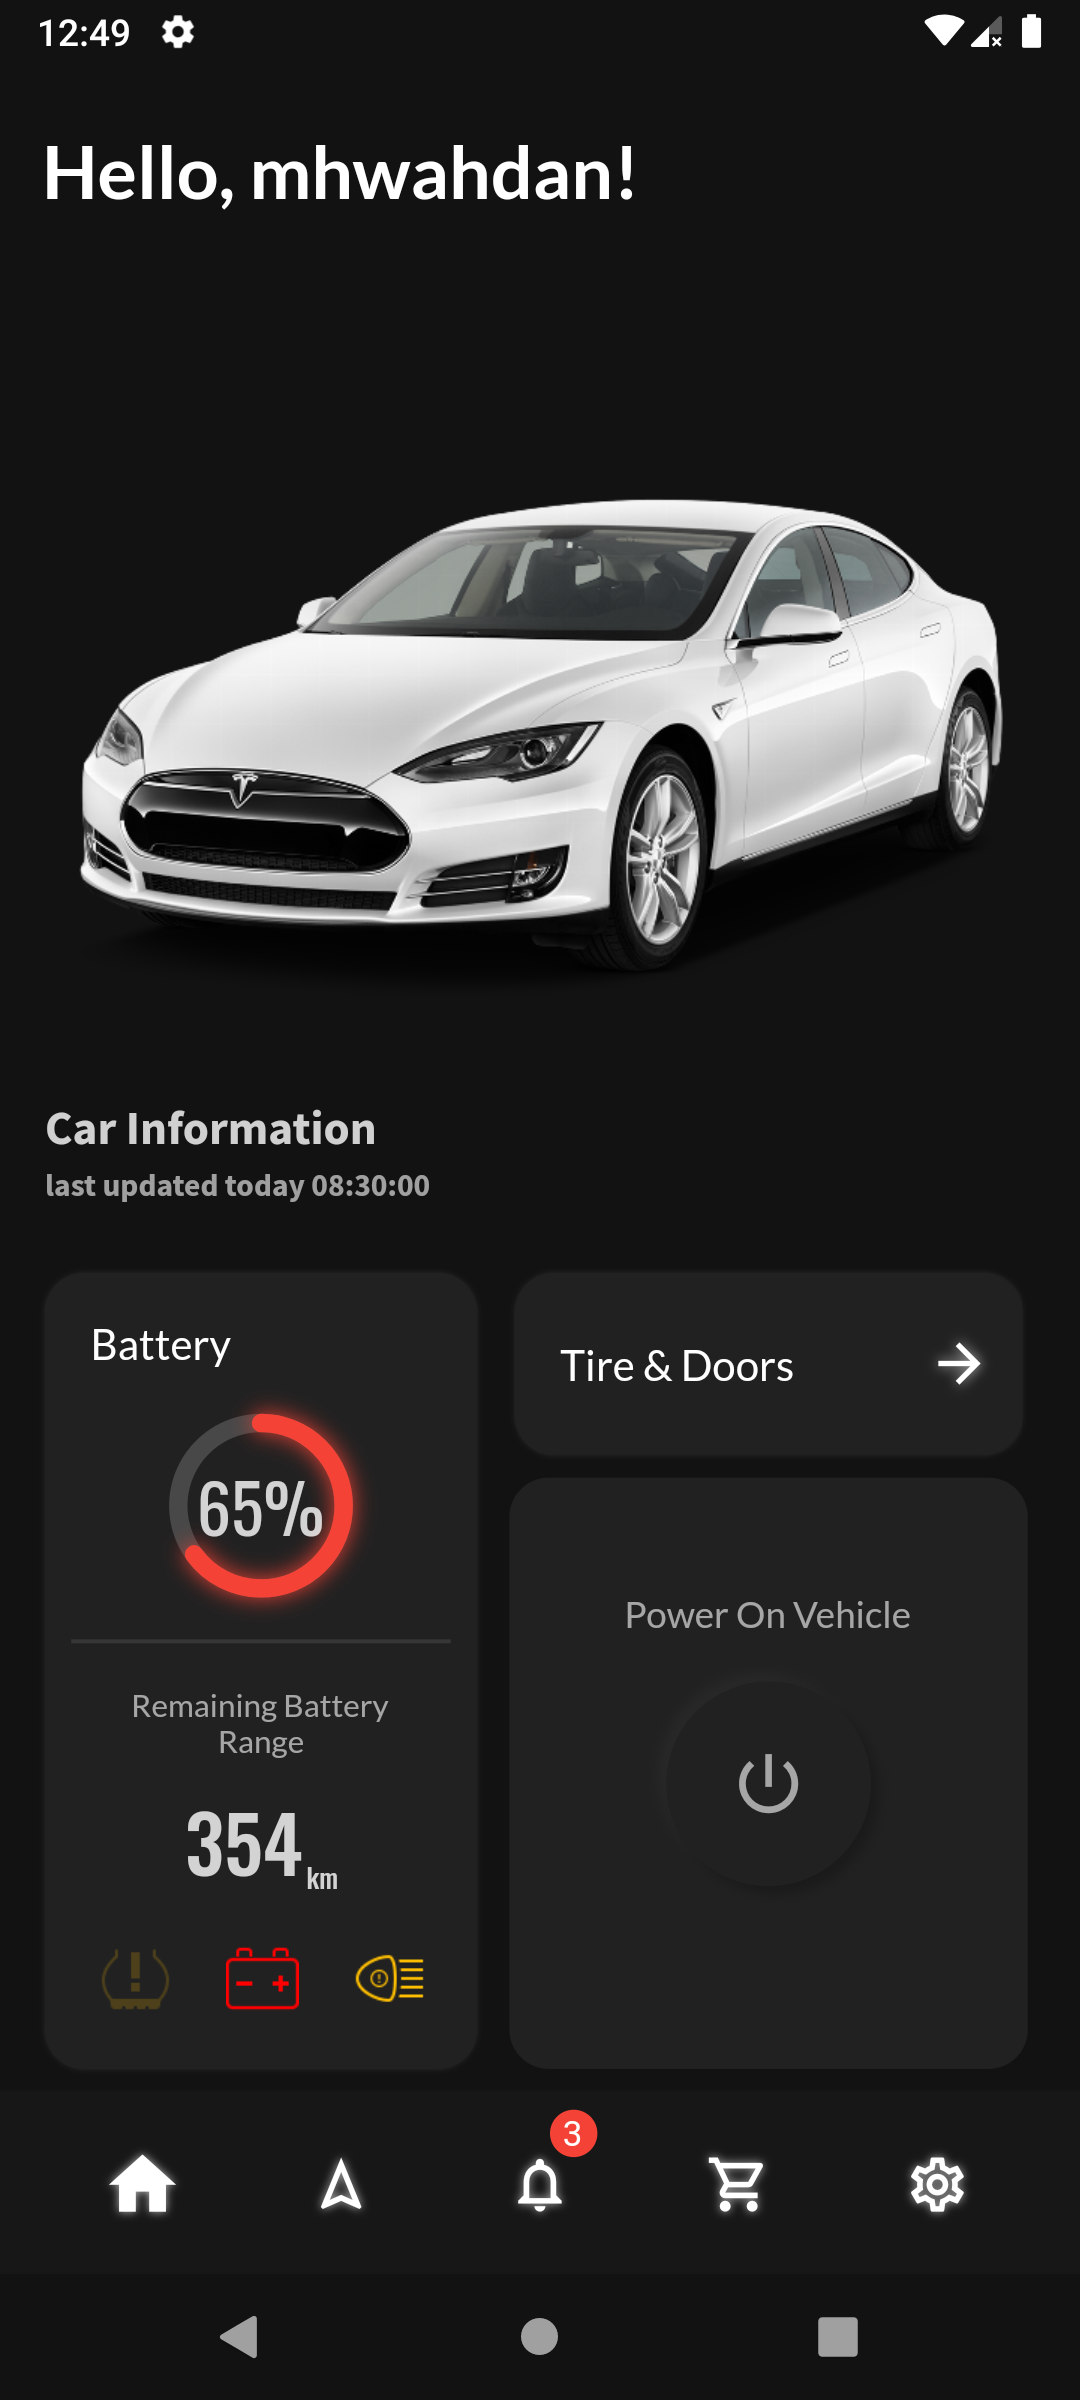
\includegraphics[scale=0.15]{Figures/mobileApp/6.png}
  	\caption{Mobile application main page}
  	\label{fig:Mobile application main page}
\end{figure}

By leveraging the secure login credentials provided during the purchasing process, primary device users can seamlessly access their accounts and gain immediate access to the app's extensive range of features and functionalities, in addition to primary device users can easily share vehicle access with their family members or grant temporary access to others. This feature enhances collaboration and convenience, allowing multiple individuals to stay connected to the vehicle's functionality and control.

Another valuable feature of our interface is the ability to track the location of the vehicle in real-time. This functionality provides users with peace of mind, knowing the whereabouts of their vehicle at any given time. Whether it's monitoring the vehicle's location for security purposes or simply keeping track of its movements, users can stay connected and in control.

Keeping users informed and empowered is another core objective of our interface. Through real-time notifications, users are promptly alerted in the event of vehicle malfunctions, ensuring quick response and prevention of further damage.

Last but not least, our mobile app interface notifies users about the availability of new software updates for their vehicles. By staying up to date with the latest software improvements, bug fixes, and feature enhancements.

\chapter{Implementation}

\section{Development model}

\subsubsection{Introduction}
The DevOps \cite{ebert2016devops} development model is a collaborative and iterative approach to software development and delivery that aims to bridge the gap between development and operations teams. It emphasizes close collaboration, continuous integration, continuous delivery, and automation to accelerate the software development lifecycle and improve overall efficiency and quality.

\begin{figure}[!ht]
	\centering
	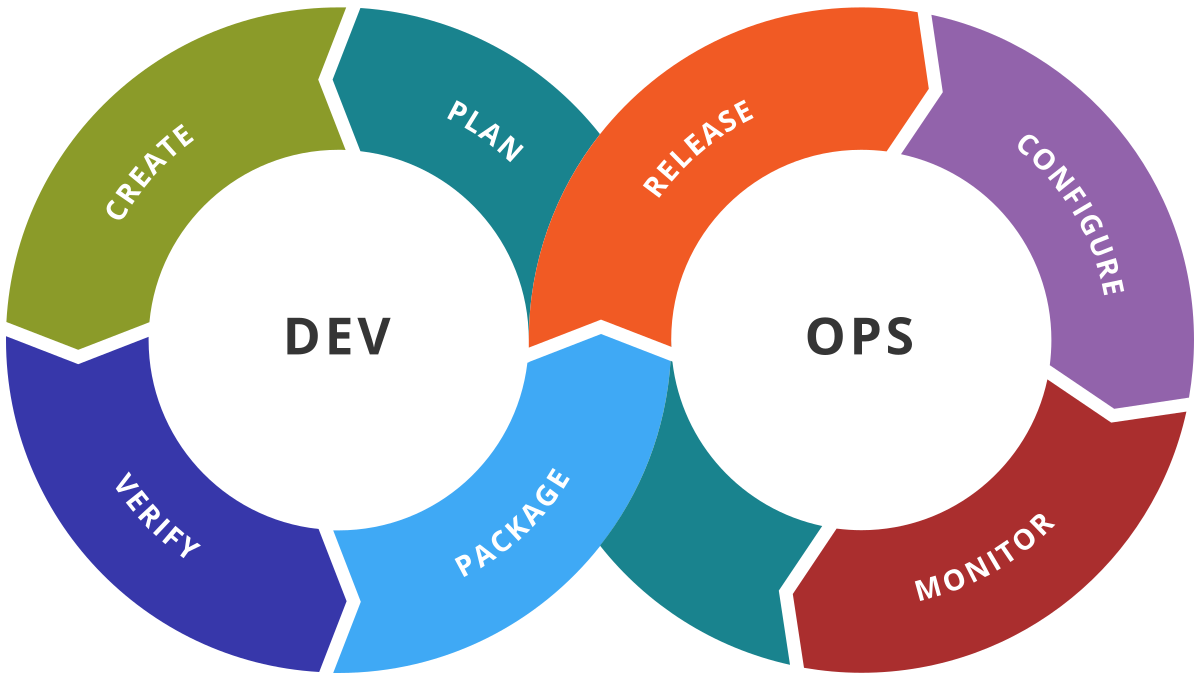
\includegraphics[scale=0.3]{Figures/DevOps/DevOps.png}
  	\caption{DevOps model}
  	\label{fig:DevOps model}
\end{figure}

At the core of the DevOps model is the integration of development and operations teams, breaking down silos and fostering a culture of shared responsibility. Development teams work closely with operations teams throughout the entire software development process, from planning and coding to testing and deployment. This collaboration allows for faster feedback loops, early identification of issues, and continuous improvement.

Continuous integration is a fundamental practice in DevOps, where developers regularly merge their code changes into a shared repository. This triggers automated build and test processes to ensure that the code-base remains in a releasable state. By integrating code changes frequently, DevOps teams can detect and address issues early on, reducing the risk of integration problems and speeding up the development cycle.

Continuous delivery is another key aspect of the DevOps model. It involves automating the software release process to enable rapid and reliable deployments. By automating tasks such as building, testing, and packaging, organizations can deliver software updates and new features more frequently and with greater confidence. This approach reduces the time and effort required for manual deployments and allows for faster feedback and iteration.

Automation is a critical component of DevOps, as it enables repeatability, consistency, and scalability. Through the use of tools and frameworks, organizations can automate various aspects of the software development and delivery process, including infrastructure provisioning, configuration management, testing, and deployment. Automation helps eliminate manual errors, reduces deployment time, and promotes a reliable and efficient work-flow.

The DevOps model also promotes a culture of continuous learning and improvement. By collecting and analyzing data from the development and operations processes, teams can gain insights into performance, identify bottlenecks, and make data-driven decisions for optimization. This culture of measurement and feedback allows organizations to continuously enhance their processes, tools, and practices.

\subsubsection{DevOps development steps}

The DevOps development model is a comprehensive and iterative approach to software development and delivery that encompasses various steps and practices. Let's explore each step in detail:

Collaboration: DevOps emphasizes the collaboration between development and operations teams. This involves breaking down silos, fostering effective communication, and aligning goals and objectives. Collaboration ensures that both teams work together throughout the software development life-cycle, sharing knowledge, expertise, and responsibilities.

Continuous Planning: DevOps begins with continuous planning, where teams define project requirements, prioritize tasks, and plan iterations or sprints. This involves close collaboration with stakeholders to ensure that business needs are met and that the development process aligns with organizational goals.

Continuous Integration (CI): Continuous integration is a core practice in DevOps. Developers integrate their code changes into a shared repository multiple times a day. This triggers automated build processes that compile the code, run unit tests, and perform static code analysis. CI helps identify integration issues early on and promotes a stable code-base.

Continuous Testing: DevOps promotes continuous testing to ensure that software meets quality standards. Automated testing frameworks are used to execute unit tests, integration tests, regression tests, and performance tests. Continuous testing helps identify defects early, validate functionality, and maintain overall software quality.

Continuous Delivery (CD): Continuous delivery is the process of automating the deployment of software updates to production-like environments. This involves creating deployment pipelines that encompass activities such as building, packaging, and deploying applications. CD ensures that software updates are readily available for release, reducing lead time and enabling frequent and reliable deployments.

Infrastructure as Code (IaC): DevOps leverages infrastructure as code, which involves using version-controlled scripts to define and manage infrastructure resources. IaC allows for the automation and reproducibility of infrastructure provisioning, configuration, and management. It ensures consistency across environments and facilitates rapid scalability.

Continuous Deployment: Continuous deployment takes continuous delivery a step further by automating the release of software updates directly into production environments. With proper testing and validation, changes are automatically deployed, reducing manual intervention and minimizing deployment time. Continuous deployment enables faster feedback loops and shorter release cycles.

Monitoring and Feedback: DevOps emphasizes continuous monitoring of software performance, user behavior, and infrastructure health. Real-time monitoring tools provide insights into application metrics, system logs, and user feedback. This feedback loop enables teams to identify and resolve issues promptly, make data-driven decisions, and continuously improve the software.

Culture of Continuous Improvement: DevOps promotes a culture of continuous learning and improvement. Teams regularly reflect on their processes, seeking ways to optimize efficiency, enhance collaboration, and adopt new technologies or practices. This culture encourages experimentation, innovation, and the adoption of best practices to drive continuous improvement.

\subsubsection{Why use the DevOps model}
There are several compelling reasons to adopt the DevOps model in software development:

1. Faster Time to Market: DevOps emphasizes automation and collaboration, enabling teams to deliver software updates more frequently and efficiently. By streamlining processes and reducing manual tasks, organizations can accelerate their time to market, responding quickly to customer demands and gaining a competitive edge.

2. Improved Collaboration and Communication: DevOps breaks down the traditional barriers between development, operations, and other stakeholders. By fostering a culture of collaboration and open communication, teams can work together more effectively, share knowledge, and align their goals. This leads to better outcomes, reduced errors, and increased efficiency.

3. Enhanced Software Quality: DevOps practices, such as continuous integration, testing, and deployment, promote early detection and resolution of issues. By automating testing processes and incorporating feedback loops, teams can identify and address defects in a timely manner. This results in improved software quality, stability, and reliability.

4. Increased Agility and Flexibility: DevOps enables organizations to quickly respond to changing business needs and market dynamics. By adopting agile practices and continuous delivery, teams can rapidly iterate and release software updates. This agility allows for faster feedback loops, faster time to value, and the ability to adapt to evolving customer requirements.

5. Scalability and Efficiency: DevOps promotes the use of infrastructure as code and automation tools, allowing organizations to scale their infrastructure and resources more efficiently. By leveraging cloud computing and containerization technologies, teams can provision and manage resources on demand, optimizing costs and improving operational efficiency.

6. Continuous Improvement: DevOps fosters a culture of continuous improvement and learning. By regularly reflecting on processes, gathering feedback, and measuring performance, teams can identify areas for optimization and implement iterative changes. This culture of continuous improvement drives innovation, increases productivity, and enhances overall performance.

7. Enhanced Customer Experience: With faster delivery cycles, improved software quality, and the ability to quickly respond to customer feedback, DevOps enables organizations to provide a better customer experience. By continuously delivering value and addressing customer needs, organizations can build trust, loyalty, and satisfaction.

Overall, the DevOps model promotes a collaborative, efficient, and customer-centric approach to software development. It enables organizations to deliver high-quality software faster, adapt to market demands, and drive innovation. By embracing DevOps principles and practices, organizations can achieve improved business outcomes and gain a competitive advantage in today's fast-paced digital landscape.
\newpage
\section{Infrastructure}

\subsection{overview}
To ensure a robust and secure infrastructure for our project, we have made the decision to utilize a cloud server combined with a firewall to host our services. This choice allows us to take advantage of the scalability, reliability, and flexibility offered by cloud computing while maintaining a strong security posture.

To implement the system architecture, we have adopted a containerized approach, where each of the four systems discussed earlier is implemented as an independent stack of containers. This containerization allows for efficient resource utilization and isolation of services, enabling easier management and deployment.

To enhance the security of our microservices, we have implemented a virtual network that facilitates internal communication between the containers. This virtual network ensures that the communication between microservices remains isolated from external threats and prevents unauthorized access, packet sniffing, or replay attacks. By utilizing this approach, we can enforce strict security boundaries and protect sensitive data and system components.

Our infrastructure design is aligned with the CAEdge architecture proposed by AWS, Amazon Web Services (AWS) is a comprehensive cloud computing platform provided by Amazon. It offers a wide range of services and solutions that enable businesses and developers to build, deploy, and manage various applications and infrastructures in the cloud.

In the context of Software Defined Vehicles (SDVs), AWS plays a significant role in providing the necessary cloud-based infrastructure and services to support SDV deployments. Following their guidelines ensures that our infrastructure meets industry best practices and is designed to handle the unique challenges and demands of automotive cloud systems.

Furthermore, our cloud server is configured with a robust firewall solution. The firewall acts as a protective barrier, monitoring and filtering incoming and outgoing network traffic based on predefined security rules. This helps safeguard our infrastructure from unauthorized access attempts, malicious activities, and potential vulnerabilities. By enforcing strict access controls and traffic filtering, we can mitigate risks and maintain the integrity and confidentiality of our services and data.

We have also implemented additional security measures, such as encryption of data in transit and at rest, secure authentication mechanisms, and regular security audits and updates. These measures ensure that our infrastructure adheres to industry security standards and safeguards against potential threats or vulnerabilities.

\subsection{Request routing}
To ensure secure and efficient request routing within our infrastructure, we have implemented NGINX as a reverse proxy. NGINX serves as a central entry point for all incoming traffic, allowing us to effectively manage and control the flow of requests to our system components. Our system is based on the API gateway proposed by CAEdge archciticture

\begin{figure}[!ht]
	\centering
	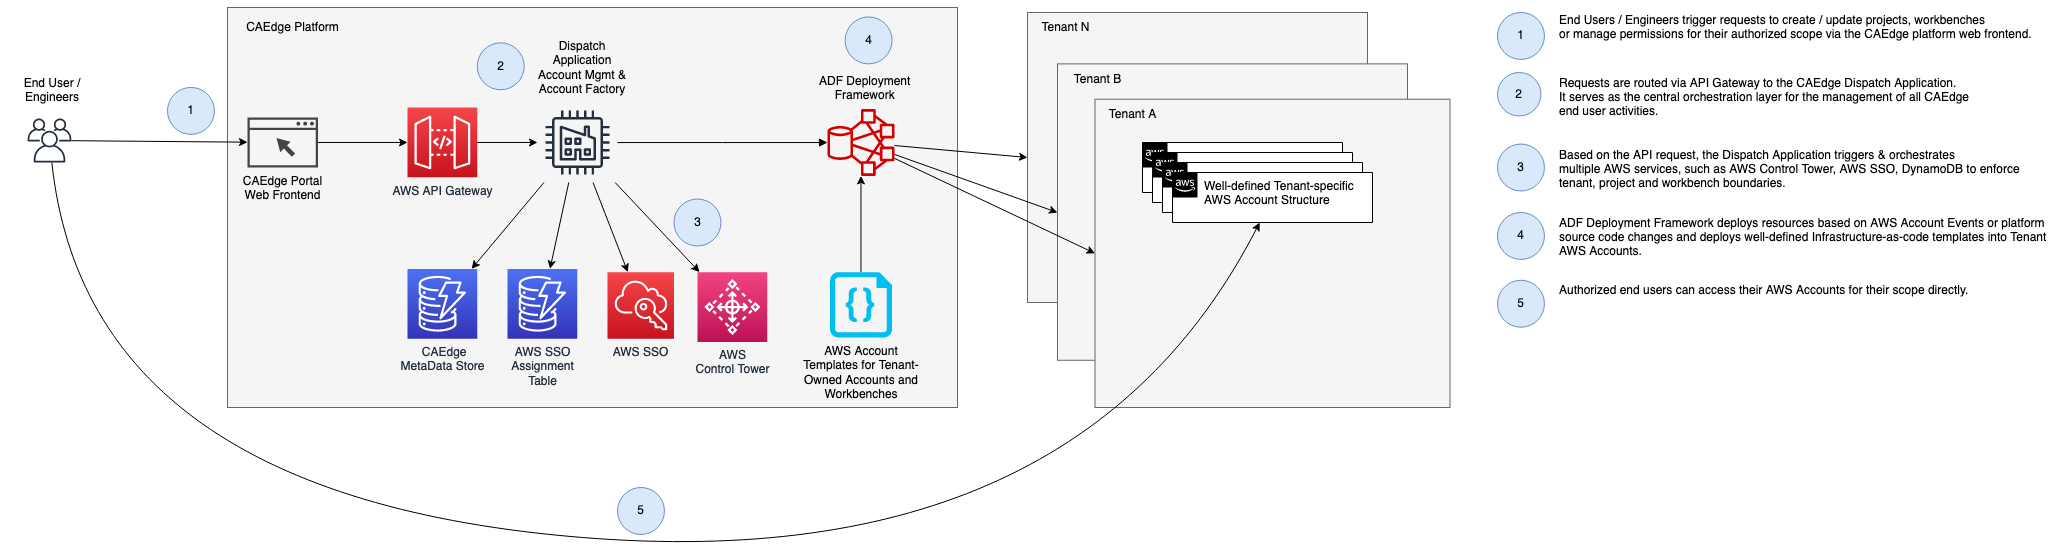
\includegraphics[scale=0.2]{Figures/Architicture/routing.png}
  	\caption{high-level overview of the automation mechanism at the platform level}
  	\label{fig:high-level overview of the automation mechanism at the platform level}
\end{figure}


One of the key advantages of using NGINX as a reverse proxy is its ability to handle SSL/TLS encryption. By terminating SSL connections at the NGINX level, we can ensure that all incoming traffic is securely encrypted. This protects sensitive data transmitted between clients and our system components, safeguarding against eavesdropping and data interception.

Furthermore, NGINX acts as a shield for our system components, preventing direct exposure to external entities. With NGINX as the single entry point, we can implement various security measures such as firewalls, authentication mechanisms, IP whitelists or blacklists, rate limiting, and other security controls. This consolidated approach simplifies the security management of our infrastructure and provides an additional layer of protection against unauthorized access and potential vulnerabilities.

NGINX also offers advanced load balancing capabilities, allowing us to distribute incoming requests across multiple instances of our system components. This helps optimize resource utilization, improve performance, and ensure high availability by evenly distributing the workload. NGINX's load balancing algorithms can be configured to suit our specific requirements and ensure efficient utilization of our system resources.

Additionally, NGINX provides extensive logging and monitoring capabilities, allowing us to track and analyze incoming traffic patterns, identify potential issues or anomalies, and make informed decisions for optimizing our system performance and security.

By leveraging NGINX as a reverse proxy, we have created a secure and controlled entry point to our infrastructure. It enables us to enforce SSL encryption, implement various security measures, and efficiently route incoming requests to the appropriate system components. This architecture ensures that our system remains protected, scalable, and highly available.

\subsection{Continuous integration and deployment}
To automate the development and deployment processes of our cloud-based system, we have implemented a CI/CD (Continuous Integration/Continuous Deployment) pipeline. This approach has significantly enhanced our development work-flow, ensuring faster and more reliable software delivery.

In our CI/CD pipeline, we have integrated several key components and tools. Firstly, we utilize a version control system, such as Git, to manage our source code repository. This enables us to maintain a centralized and organized code-base, facilitating collaboration among developers and ensuring version control.

Next, we have set up a build automation tool, such as Jenkins, which orchestrates the CI process. Whenever changes are pushed to the repository, Jenkins automatically triggers a build process, compiling the code, running tests, and generating build artifacts. This ensures that each code change is thoroughly tested and validated, maintaining code quality and reducing the likelihood of introducing bugs or issues.

Following successful builds, the artifacts are deployed to various environments, such as staging or production, using our deployment automation tool. This tool, like Ansible or Kubernetes, enables us to define and manage the infrastructure and configuration required for running our cloud-based system. It automates the provisioning and deployment of the necessary resources, ensuring consistency and reproducibility across different environments.

Additionally, we incorporate automated testing into our CI/CD pipeline. This includes unit tests, integration tests, and even end-to-end tests, depending on the complexity of our system. Automated testing helps identify any regressions or issues early on, ensuring the stability and reliability of our cloud-based system.

To further enhance our CI/CD pipeline, we integrate various monitoring and logging tools. These tools provide real-time insights into the performance, availability, and health of our system, allowing us to promptly detect and address any issues that may arise.

Overall, by implementing CI/CD in automating the development of our cloud-based system, we have achieved significant benefits. We have streamlined our development process, enabling rapid iterations and quicker delivery of new features and bug fixes. The automation ensures consistency, repeatability, and reliability in our deployments, reducing the risk of human error. This approach also promotes collaboration among developers, as it encourages frequent code integration and collaboration through version control. Ultimately, our CI/CD pipeline has significantly improved the overall efficiency, quality, and agility of our cloud-based system development.

\section{Tools and frameworks}

\subsection{PostgreSQL}

\subsubsection{What is postgreSQL}

PostgreSQL \cite{momjian2001postgresql} is a robust and feature-rich open-source relational database management system (RDBMS) that offers reliability, scalability, and advanced functionality. With its strong reputation for data integrity and stability, PostgreSQL is an excellent choice for applications of all sizes. It provides a wide range of features, including support for complex queries, advanced data types, and efficient indexing. PostgreSQL is highly extensible, allowing developers to customize and tailor the database to their specific needs. Its active and supportive community ensures ongoing development, support, and a wealth of resources.

\begin{figure}[!ht]
	\centering
	
\includegraphics[scale=0.5]{Figures/database/postgreSQL.png}
  	\caption{PostgreSQL}
  	\label{fig:PostgreSQL}
\end{figure}

\subsubsection{why PostgreSQL?}

\begin{itemize}
\item \textbf{Reliability and Stability:} PostgreSQL is known for its reliability and stability. It has a reputation for being a robust and secure database that provides consistent and accurate data storage.

\item \textbf{Advanced Features:} PostgreSQL offers a wide range of advanced features that make it suitable for handling complex data requirements. It supports various data types, including JSON, arrays, and geospatial data, allowing you to store and query diverse types of information. Additionally, PostgreSQL provides advanced indexing techniques, full-text search capabilities, and support for complex queries, making it a powerful choice for data-intensive applications.

\item \textbf{Scalability and Performance:} PostgreSQL is designed to handle high volumes of data and demanding workloads. It supports parallel processing, allowing multiple queries to be executed simultaneously and taking advantage of multi-core processors. Additionally, PostgreSQL provides efficient indexing, query optimization, and caching mechanisms to deliver excellent performance even for complex queries.

\item \textbf{Platform Independence:} PostgreSQL is platform-independent and runs on various operating systems, including Windows, macOS, and Linux.
\end{itemize}

\subsection{.NET Core}
\subsubsection{What is .NET Core}

ASP.NET Core is a cross-platform framework that enables developers to build web applications that can run on different operating systems, including Windows, macOS, and Linux. It offers a unified programming model that combines the best features from earlier versions of ASP.NET, making it easier to create scalable, high-performance web applications.

\begin{figure}[!ht]
	\centering
	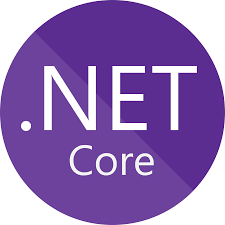
\includegraphics[scale=0.5]{Figures/Backend/asp-net-core.png}
  	\caption{.NET Core}
  	\label{fig:.NET Core}
\end{figure}

\subsubsection{Why .NET 6?}

\begin{itemize}
\item \textbf{Cross-Platform Compatibility:} .NET 6 allows developers to build web applications that can run on different operating systems, providing flexibility and enabling developers to choose their preferred development environment.

\item \textbf{High Performance:} .NET 6 is optimized for performance, offering a lightweight and modular architecture that reduces overhead and enhances the speed of request processing.

\item \textbf{Cloud-Native and Microservices Support:} .NET is designed to be cloud-native, making it well-suited for building applications that run in cloud environments. It provides integration with popular cloud platforms, containerization technologies, and DevOps practices.

\item \textbf{Identity Schema:} The Identity Schema in ASP.NET Core provides a standardized system for managing user authentication and authorization. It includes features for user registration, login, password management, and role-based access control. The Identity Schema defines a set of tables and relationships that store user-related information in a data store, such as a relational database. It provides a robust and extensible framework for implementing user authentication and authorization in web applications.

\item \textbf{Authorization Policies:} ASP.NET Core 6 includes a flexible and robust authorization system. It allows you to define fine-grained access control rules using attributes, policies, or custom requirements. You can easily implement role-based access control (RBAC), claims-based authorization, or any other custom authorization scheme based on your application's requirements.

\item \textbf{Built-in Dependency Injection:} ASP.NET Core includes a built-in dependency injection (DI) framework that promotes loose coupling and improves the maintainability and testability of your code.
\end{itemize}


\subsection{Flutter}
\subsubsection{What is Flutter}

Flutter is an open-source user interface framework developed by Google. It enables developers to create high-quality applications across multiple platforms using a single code-base. Flutter provides a comprehensive set of tools, libraries, and widgets to assist developers in building applications. It utilizes the Dart programming language, also developed by Google, which focuses on performance, productivity, and scalability. Flutter leverages Dart's features to provide a reactive and component-based architecture for creating user interfaces.


\begin{figure}[!ht]
	\centering
	
\includegraphics[scale=0.5]{Figures/FrontEnd/MobileApplication/flutter.png}
  	\caption{Flutter}
  	\label{fig:Flutter}
\end{figure}
\subsubsection{why Flutter?}

Flutter follows a different approach compared to traditional frameworks by rendering its own UI instead of relying on native components of the operating system. It uses a 2D rendering engine called Skia, which allows Flutter to deliver smooth animations, transitions, and a consistent user experience across different platforms.

\textbf{Key Points:}

\begin{itemize}
\item \textbf{Cross-Platform Development:} With Flutter, developers can create code once and deliver it across multiple platforms, including iOS, Android, web, and desktop. This eliminates the need to maintain different codebases for each platform, reducing development time and effort.

\item \textbf{Dart Programming Language:} Flutter utilizes Dart as its programming language. Dart provides modern features such as Just-in-Time (JIT) compilation during development and Ahead-of-Time (AOT) compilation during production, enabling efficient code execution.

\item \textbf{Reactive Framework:} Flutter employs a reactive framework where the user interface (UI) is automatically updated in response to changes in the underlying data. This allows for the creation of engaging and responsive user interfaces.

\item \textbf{Hot Reload:} Flutter's hot reload feature enables developers to see the changes they make in the code immediately reflected in the app. This speeds up the development process by providing instant feedback and reducing the time required for testing and debugging.

\item \textbf{Rich Set of Widgets:} Flutter offers a wide range of pre-designed widgets for building UI elements such as buttons, text fields, images, navigation, and more. These widgets can be customized and combined to create rich and interactive user interfaces.

\item \textbf{Fast Performance:} Flutter apps are compiled to native machine code, resulting in exceptional speed. The Skia rendering engine used by Flutter directly renders UI elements, ensuring fluid animations and a responsive user interface.
\end{itemize}


\subsection{Angular}
\subsubsection{What is Angular}

Angular is an open-source front-end framework developed by Google for building dynamic web applications. It is a comprehensive framework that provides a rich set of tools and features to simplify the development process and create powerful applications.

Angular follows a component-based architecture, where applications are built as a collection of reusable and modular components. These components encapsulate their own templates, styles, and logic, making them self-contained and easy to manage. With Angular's declarative templates and powerful data binding, it is easy to create dynamic and interactive user interfaces, which made it the best choice for our project.

\begin{figure}[!ht]
	\centering
	
\includegraphics[scale=0.5]{Figures/FrontEnd/AdminConsole/angular.png}
  	\caption{Angular}
  	\label{fig:Angular}
\end{figure}

\subsubsection{Why Angular?}

\begin{itemize}
\item \textbf{Full-Featured Framework:} Angular is a full-featured framework that provides everything to build complex web applications. It offers a powerful templating system, a modular architecture, component-based development, and a rich set of built-in libraries and tools.

\item \textbf{Single-page application (SPA):} Angular is particularly well-suited for building SPAs due to its component-based architecture and powerful routing capabilities. The component-based architecture allows developers to break down the application into modular components, each responsible for its own functionality and user interface. These components can be dynamically loaded and updated based on user interactions, resulting in a seamless and interactive application flow.

\item \textbf{TypeScript Language:} Angular is built using TypeScript, a statically typed superset of JavaScript. TypeScript brings additional features to JavaScript, such as static type checking, enhanced tooling, and improved maintainability. It helps catch errors at compile-time and provides better code organization and refactoring capabilities.

\item \textbf{Cross-Platform Development:} Angular supports cross-platform development, allowing you to build applications that run seamlessly on various platforms, including web browsers, desktops, and mobile devices.

\item \textbf{Integration with Other Technologies:} Angular integrates well with other technologies and libraries, allowing developers to leverage existing tools and resources. It can be easily integrated with popular libraries like RxJS for reactive programming, Redux for state management, and third-party UI component libraries like Material Design for ready-to-use UI elements.
\end{itemize}

\subsection{Docker}
\subsubsection{What is Docker}
Docker is an open-source containerization platform that allows developers to package applications and their dependencies into lightweight and portable containers. Containers are isolated environments that encapsulate an application and all its dependencies, including libraries, frameworks, and system tools. Docker simplifies the process of deploying and running applications by providing a consistent and reproducible environment across different systems and platforms. With Docker, developers can create a container image that contains all the necessary components for their application to run, ensuring that it behaves consistently regardless of the underlying infrastructure. These container images can be easily shared, versioned, and deployed to any Docker-compatible environment, making application deployment faster and more efficient. Docker also provides a powerful set of tools and features for managing and orchestrating containers, such as Docker Compose for defining multi-container applications and Docker Swarm or Kubernetes for container orchestration at scale. By leveraging Docker, developers can achieve greater flexibility, scalability, and efficiency in their application development and deployment processes.

\begin{figure}[!ht]
	\centering
	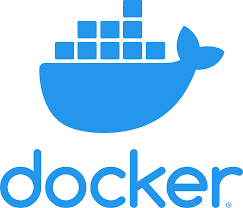
\includegraphics[scale=0.5]{Figures/DevOps/docker.png}
  	\caption{Docker}
  	\label{fig:Docker}
\end{figure}
\subsubsection{Why use docker ?}
Containerization: Docker is a containerization platform that enables developers to package applications and their dependencies into self-contained, lightweight containers. Containers are isolated environments that encapsulate an application's code, runtime, system tools, libraries, and configurations. This isolation ensures that the application runs consistently and reliably across different environments, regardless of the underlying infrastructure.

Portability: Docker provides a high level of portability for applications. Containers can be created once and run on any Docker-compatible system, including laptops, servers, virtual machines, and cloud platforms. This portability eliminates the "it works on my machine" problem and enables seamless deployment across different environments.

Efficiency and Resource Utilization: Docker containers are lightweight and consume fewer resources compared to traditional virtual machines (VMs). They share the host system's kernel and only require resources necessary for the application to run, making them more efficient and enabling higher resource utilization. Docker also allows multiple containers to run on the same host system, improving overall system efficiency.

Isolation and Security: Docker containers provide a high level of isolation, ensuring that applications and their dependencies do not interfere with each other. Each container runs in its own isolated environment, separate from the host system and other containers. This isolation enhances security by preventing unauthorized access and reducing the impact of potential security vulnerabilities.

Versioning and Image Management: Docker uses a layered approach to container images. Each layer represents a specific component or change in the image. Docker images can be versioned, allowing developers to track changes and easily roll back to previous versions if needed. Docker also supports image registries, such as Docker Hub, where developers can store and share their container images with others.

Scalability and Orchestration: Docker provides tools for scaling applications and managing containerized environments. Docker Swarm and Kubernetes are popular container orchestration platforms that allow for the deployment, scaling, and management of containers across a cluster of machines. These tools enable applications to scale horizontally by dynamically allocating and managing containers based on demand.

DevOps Integration: Docker plays a crucial role in the DevOps workflow. It enables developers to create reproducible environments that closely mirror production environments. Docker images can be used in continuous integration and delivery (CI/CD) pipelines, allowing for seamless deployment and testing of applications. Docker also facilitates collaboration between development and operations teams, as the same containerized environment can be used throughout the development, testing, and production stages.

Ecosystem and Community: Docker has a vast ecosystem and an active community of developers, providing a wealth of resources, tutorials, and pre-built images. Docker Hub, the official registry, hosts thousands of pre-built images that can be used as a starting point for building containerized applications. The Docker community constantly contributes to the platform's development, ensuring continuous improvement and support.
\newpage
\subsection{EMQX}
\subsubsection{What is EMQX}
EMQX is an open-source, highly scalable, and extensible MQTT broker that is designed for handling massive concurrent connections and real-time message delivery. MQTT (Message Queuing Telemetry Transport) is a lightweight messaging protocol widely used in Internet of Things (IoT) and real-time communication applications.

EMQX provides a robust and efficient MQTT broker implementation that enables devices and applications to publish and subscribe to messages in a distributed and scalable manner. It supports MQTT versions 3.1 and 3.1.1, as well as MQTT-SN (MQTT for Sensor Networks) and MQTT over WebSocket protocols.

\begin{figure}[!ht]
	\centering
	
\includegraphics[scale=0.5]{Figures/Backend/EMQX.png}
  	\caption{EMQX}
  	\label{fig:EMQX}
\end{figure}

\subsubsection{Why use EMQX ?}
High Scalability: EMQX is built to handle a massive number of concurrent connections and deliver messages in real-time. It is designed to support millions of concurrent MQTT connections, making it suitable for IoT deployments and applications with high scalability requirements.

Clustering and Load Balancing: EMQX supports clustering, allowing multiple EMQX nodes to work together as a unified MQTT broker system. Clustering enables horizontal scaling and load balancing across nodes, ensuring high availability and improved performance.

Message Routing and Filtering: EMQX provides flexible message routing and filtering capabilities. It supports topic-based message routing, where messages are delivered to subscribers based on their subscribed topics. EMQX also supports custom plugins and rules for advanced message filtering and processing.

QoS (Quality of Service) Support: EMQX supports all three levels of MQTT Quality of Service (QoS): QoS 0 (at most once), QoS 1 (at least once), and QoS 2 (exactly once). This allows applications to choose the appropriate level of message reliability based on their requirements.

Security: EMQX offers various security features to protect MQTT communications. It supports Transport Layer Security (TLS) encryption for secure communication over the network. EMQX also provides authentication and authorization mechanisms, including username/password-based authentication and access control lists (ACLs) to ensure only authorized clients can connect and access specific topics.

Real-time Metrics and Monitoring: EMQX provides real-time metrics and monitoring capabilities to monitor the health and performance of the MQTT broker. It supports integration with monitoring tools such as Prometheus and Grafana, allowing users to visualize and analyze the broker's metrics.

Extensibility and Plugin System: EMQX offers an extensible architecture with a plugin system that allows developers to extend its functionality. Custom plugins can be developed to add new features, integrate with external systems, or customize the behavior of the MQTT broker.

\subsection{Portainer}

\subsubsection{What is portainer}

Portainer is a user-friendly, open-source container management platform that simplifies the deployment and management of Docker containers. With Portainer, users can easily create, configure, and monitor containerized applications through a web-based interface. It provides a graphical user interface (GUI) that abstracts the complexity of working with Docker, making it accessible to both novice and experienced users.

\subsubsection{Why Portainer ?}

One of the key features of Portainer is its intuitive dashboard, which provides a centralized view of all containers, images, volumes, and networks. From the dashboard, users can start, stop, restart, and remove containers with a few clicks. They can also manage container networks, inspect logs, and access container terminals directly from the web interface.

Portainer supports multi-host environments, allowing users to manage Docker installations across different machines from a single Portainer instance. It provides seamless integration with Docker Swarm, enabling users to deploy and manage swarm services and stacks.

Furthermore, Portainer offers role-based access control (RBAC), allowing administrators to define granular access permissions for different users and teams. This ensures that each user has the appropriate level of access and control over the Docker resources.

Portainer also supports the management of Docker-compose files, which allows users to define and deploy multi-container applications using a declarative configuration file. This simplifies the process of managing complex applications with multiple containers and their interdependencies.

Overall, Portainer serves as a powerful tool for managing Docker containers, providing an intuitive interface, multi-host support, RBAC, and integration with Docker Swarm and Docker-compose. Whether used by individuals, small teams, or enterprise environments, Portainer streamlines the container management process, making it easier to deploy and maintain containerized applications.

\subsection{NGINX}
\subsubsection{What is NGINX}

NGINX is a popular open-source web server and reverse proxy server that is widely used for hosting websites, serving static content, and load balancing. It is known for its high performance, scalability, and robustness, making it a preferred choice for many developers and administrators.

\begin{figure}[!ht]
	\centering
	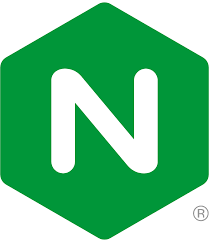
\includegraphics[scale=0.5]{Figures/Backend/nginx.png}
  	\caption{NGINX}
  	\label{fig:NGINX}
\end{figure}

\subsubsection{Why NGINX ?}
One of the key features of NGINX is its ability to handle a large number of concurrent connections efficiently. It uses an event-driven architecture, which allows it to handle multiple connections simultaneously without consuming excessive system resources. This makes NGINX well-suited for high traffic websites and applications.

NGINX can also act as a reverse proxy server, which means it can receive client requests and forward them to backend servers. This enables load balancing and improves the overall performance and availability of web applications. NGINX supports various load balancing algorithms, such as round-robin, least connections, and IP hash, allowing administrators to distribute the incoming requests evenly among multiple backend servers.

Another notable feature of NGINX is its support for caching static content. It can cache frequently accessed files in memory, reducing the load on backend servers and improving response times for subsequent requests. This caching mechanism can significantly improve the performance of websites and reduce server load.

NGINX also provides advanced features for URL rewriting, SSL/TLS termination, and gzip compression. It supports flexible configuration options, allowing administrators to customize the server behavior based on their specific requirements. NGINX configurations are written in a concise and readable syntax, making it easier to manage and maintain complex server setups.

Furthermore, NGINX has a large and active community of developers and users who contribute to its development and provide support. It has extensive documentation and a wide range of modules and plugins that extend its functionality and integration with other technologies.

Overall, NGINX is a powerful and versatile web server and reverse proxy server that offers high performance, scalability, and advanced features. Its ability to handle large numbers of concurrent connections, act as a reverse proxy, cache static content, and provide flexible configuration options make it a popular choice for hosting websites and improving web application performance.

\subsection{Jenkins}
\subsubsection{What is Jenkins}
Jenkins is an open-source automation server that provides a platform for continuous integration (CI) and continuous delivery (CD) processes. It is widely used in software development to automate the building, testing, and deployment of applications. Jenkins offers a robust and flexible framework that enables developers to streamline their development workflows and ensure the delivery of high-quality software.
\begin{figure}[!ht]
	\centering
	
\includegraphics[scale=0.5]{Figures/DevOps/jenkins.png}
  	\caption{Jenkins}
  	\label{fig:Jenkins}
\end{figure}
\subsubsection{Why Jenkins ?}
One of the key features of Jenkins is its ability to automate the entire software development lifecycle. It allows developers to define pipelines, which are sequences of steps that specify how code should be built, tested, and deployed. These pipelines can be easily customized and adapted to meet specific project requirements. Jenkins supports various types of pipelines, including declarative and scripted pipelines, giving developers flexibility in defining their work-flows.

Jenkins integrates seamlessly with version control systems, such as Git, allowing it to monitor changes in the code repository and trigger automated builds and tests whenever changes are detected. It supports a wide range of build tools, testing frameworks, and deployment technologies, making it compatible with diverse development environments.

Another important feature of Jenkins is its extensive plugin ecosystem. Jenkins provides a vast collection of plugins that extend its functionality and enable integration with other tools and services. These plugins cover various areas, including source code management, build tools, testing frameworks, deployment technologies, and notification systems. The plugin ecosystem allows developers to easily integrate Jenkins with their existing development stack and customize it according to their specific needs.

Jenkins also provides a user-friendly web interface that allows developers to manage and monitor their builds, view detailed reports and logs, and configure various settings. The web interface provides real-time updates on the status of builds and tests, making it easy to identify and troubleshoot any issues that arise during the development process.

Furthermore, Jenkins supports distributed builds, allowing developers to distribute the workload across multiple machines or agents. This enables faster build times and better resource utilization, particularly in large-scale projects.

Jenkins has a strong and active community of developers who contribute to its development, create plugins, and provide support to users. It has extensive documentation, tutorials, and a vibrant online community, making it easy for developers to get started with Jenkins and find solutions to their problems.

In summary, Jenkins is a powerful automation server that facilitates continuous integration and continuous delivery processes in software development. Its ability to automate builds, tests, and deployments, along with its plugin ecosystem, flexible pipelines, and distributed build support, make it a valuable tool for improving development work-flows and ensuring the delivery of high-quality software.
\newpage
\subsection{GIT}

\subsubsection{What is Git}
Git is a distributed version control system (VCS) that allows developers to track changes, collaborate on projects, and manage source code efficiently. It was created by Linus Torvalds, the creator of Linux, and has become one of the most widely used VCS in the software development industry.

\begin{figure}[!ht]
	\centering
	\includegraphics[scale=0.5]{Figures/DevOps/GIT.png}
  	\caption{GIT}
  	\label{fig:GIT}
\end{figure}

\subsubsection{Why GIT ?}

One of the key advantages of Git is its distributed nature. Each developer working on a project has a complete copy of the repository, including its full history. This means that developers can work offline and independently, making local commits, branching, and merging without the need for a centralized server. Git's distributed architecture also provides redundancy and enables easy collaboration between team members.

Git offers a lightweight and fast approach to version control. It uses a directed acyclic graph to represent the commit history, which allows for efficient branching and merging. Git employs a snapshot-based model, storing the entire state of the project at each commit, rather than just the changes. This approach ensures integrity and enables fast retrieval of previous versions.

Branching and merging are fundamental features of Git. Developers can create branches to work on specific features or bug fixes, making it easy to isolate changes and collaborate on different tasks simultaneously. Merging branches in Git is straightforward and allows for the integration of changes from one branch into another, ensuring a smooth and controlled process of incorporating new features or bug fixes into the main codebase.

Git provides robust tools for resolving conflicts that may arise when merging branches. When multiple developers make conflicting changes to the same file, Git helps identify the conflicts and allows developers to resolve them manually. This enables efficient collaboration and prevents code conflicts from disrupting the development process.

Another powerful feature of Git is its support for decentralized work-flows. Git allows developers to set up multiple remotes, which are remote repositories where the code can be stored and shared. This enables teams to collaborate across different locations and work on their own copies of the project, syncing changes with other team members when necessary.

Git integrates seamlessly with popular code hosting platforms like GitHub, GitLab, and Bitbucket. These platforms provide a centralized location to host Git repositories, facilitate collaboration, and offer additional features like issue tracking, pull requests, and code reviews.

In summary, Git is a versatile and powerful version control system that provides developers with the ability to track changes, collaborate effectively, and manage source code efficiently. Its distributed nature, branching and merging capabilities, conflict resolution tools, and integration with code hosting platforms make it an essential tool in modern software development workflows.
\newpage
\subsection{Linux}
\subsubsection{What is Linux}
Linux is an open-source operating system that is widely used in a variety of computing devices, from servers and desktop computers to mobile devices and embedded systems. It was initially created by Linus Torvalds in 1991 and has since become a leading choice for developers, businesses, and individuals due to its stability, flexibility, and security.

\begin{figure}[!ht]
	\centering
	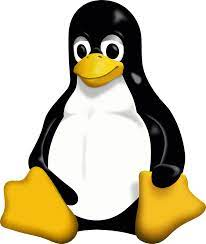
\includegraphics[scale=0.5]{Figures/DevOps/linux.jpeg}
  	\caption{Linux}
  	\label{fig:Linux}
\end{figure}
\subsubsection{Why Linux ?}
One of the key features of Linux is its kernel, which serves as the core component of the operating system. The Linux kernel provides essential functionalities, such as managing hardware resources, memory management, process scheduling, and device drivers. It is designed to be highly efficient and scalable, capable of running on a wide range of hardware architectures.

Linux distributions, also known as distros, are complete operating systems built around the Linux kernel. They come with additional software packages, utilities, and desktop environments, providing a user-friendly interface and a comprehensive set of tools for various purposes. Some popular Linux distributions include Ubuntu, Fedora, Debian, CentOS, and Arch Linux.

One of the major advantages of Linux is its open-source nature. Being open source means that the source code of the operating system is freely available, allowing users and developers to study, modify, and distribute it. This fosters a collaborative and transparent development environment, leading to constant improvements, bug fixes, and security enhancements.

Linux is known for its stability and reliability. It has a reputation for running for extended periods without the need for frequent reboots or experiencing system crashes. This stability is particularly valuable in server environments, where uninterrupted operation is crucial.

Linux provides a high level of customization and flexibility. Users can choose from various desktop environments, such as GNOME, KDE, XFCE, or LXDE, to tailor their user experience. Additionally, the modular nature of Linux allows users to install and configure only the software and components they need, optimizing system performance and resource utilization.

Security is a fundamental aspect of Linux. The open-source nature of the operating system allows for continuous security audits, prompt vulnerability fixes, and the development of robust security measures. Additionally, Linux benefits from a strong community of developers and users who actively contribute to security enhancements and share best practices.

Linux has excellent support for networking and server-related tasks. It is widely used as a platform for web servers, database servers, file servers, and networking devices due to its stability, scalability, and performance. Linux also offers a wide range of server-oriented tools and technologies, such as the Apache web server, MySQL and PostgreSQL databases, and the OpenSSH secure shell protocol.

Furthermore, Linux provides compatibility with a vast array of software applications and programming languages. Many popular applications, including web browsers, office suites, multimedia tools, and development environments, have versions specifically developed for Linux. Additionally, Linux has extensive support for various programming languages, making it an attractive platform for software developers.

In conclusion, Linux is a powerful, reliable, and versatile operating system that offers a wide range of benefits. Its open-source nature, stability, flexibility, security features, and extensive software ecosystem have contributed to its widespread adoption in diverse computing environments. Whether used by individuals, businesses, or organizations, Linux provides a solid foundation for efficient and secure computing.
\newpage
\section{Data Center}
In our project, we have chosen PostgreSQL as the database system to serve as the backbone for our system services. PostgreSQL is a powerful open-source relational database management system known for its reliability, scalability, and advanced features. It offers robust transaction support, data integrity, and ACID (Atomicity, Consistency, Isolation, Durability) compliance, making it suitable for handling complex data interactions.

By utilizing PostgreSQL, we ensure the persistence and efficient management of our system's data. All our system services communicate with the PostgreSQL database through a secure internal network. This internal network provides a protected and isolated environment, preventing unauthorized access and potential security breaches.

The use of PostgreSQL enables seamless and efficient data exchange between our system components. Our services can store, retrieve, and update data within the database, ensuring data consistency and integrity across the system. This centralization of data allows for efficient querying and analysis, facilitating real-time decision-making and providing a foundation for system optimization and performance monitoring.

Furthermore, PostgreSQL's support for advanced features such as indexing, replication, and complex querying capabilities enhances the overall functionality and performance of our system. It allows us to implement efficient data retrieval and manipulation operations, improving response times and ensuring smooth system performance even under high loads.

In terms of security, PostgreSQL provides various mechanisms to protect data within the database. It supports authentication and authorization mechanisms, allowing us to control access to sensitive data and enforce strict security policies. Additionally, PostgreSQL offers encryption options to ensure data privacy and confidentiality, adding an extra layer of protection to our system.

Overall, the utilization of PostgreSQL as our database system, combined with secure internal network communication, ensures the reliability, scalability, and security of our system's data. It provides a solid foundation for data storage, retrieval, and management, enabling efficient and secure interactions between our system services and facilitating the smooth operation of our project.

\section{Authentication and authorization}

\subsection{Mobile Authentication}
The mobile authentication process serves as a vital gateway, ensuring secure access and safeguarding sensitive user data. It focuses on ensuring that only authorized individuals with valid credentials and access privileges can gain entry to their accounts. It requires primary devices users to log in using their credentials along with one-time password through their email. The purpose of incorporating the email verification method is to add an extra level of protection and enhance the security of the authentication process. On the other hand, secondary devices can log in by scanning the QR code provided by the primary device.

\subsubsection{Primary device authentication}
The primary device login feature allows users to securely access their accounts on their mobile application. During the login process, users are required to enter their unique identifiers which includes username/email and password. These credentials are transmitted securely to the authentication server, where it is verified against stored user credentials. By enforcing the usage of primary devices for credential input, the feature ensures that only authorized individuals possessing the correct login information can successfully authenticate and gain access to their accounts, also a one-time password sent to user’s mail is required within a specified timeframe. This approach enhances the security of user accounts, safeguarding sensitive information stored within them and providing an additional barrier against potential account breaches.


\begin{enumerate}
\item Flutter Implementation.
\begin{itemize}
\item The mobile app includes a login screen where users enter their username/email and password.
\item Upon tapping the Login button, the application sends an HTTP POST request using the Dio package to "/authentication/mobile/login".
\item The request body includes the user credentials in JSON format.
\item Upon successful login, the mobile app will receive a JSON Web token (JWT) from the backend and store it locally for subsequent requests.
\item Then the app directs the user to the OTP verification screen and requires the user to enter a 4-digit OTP code received by their email.
\item Upon tapping the Verify button, the application sends an HTTP POST request to the "/authentication/mobile/verifymail" endpoint of the back-end.
\item If the backend server responds with a status code of 200, the mobile app will direct the user to the main page.
\end{itemize}
\end{enumerate}

\begin{figure}[!ht]
	\centering
	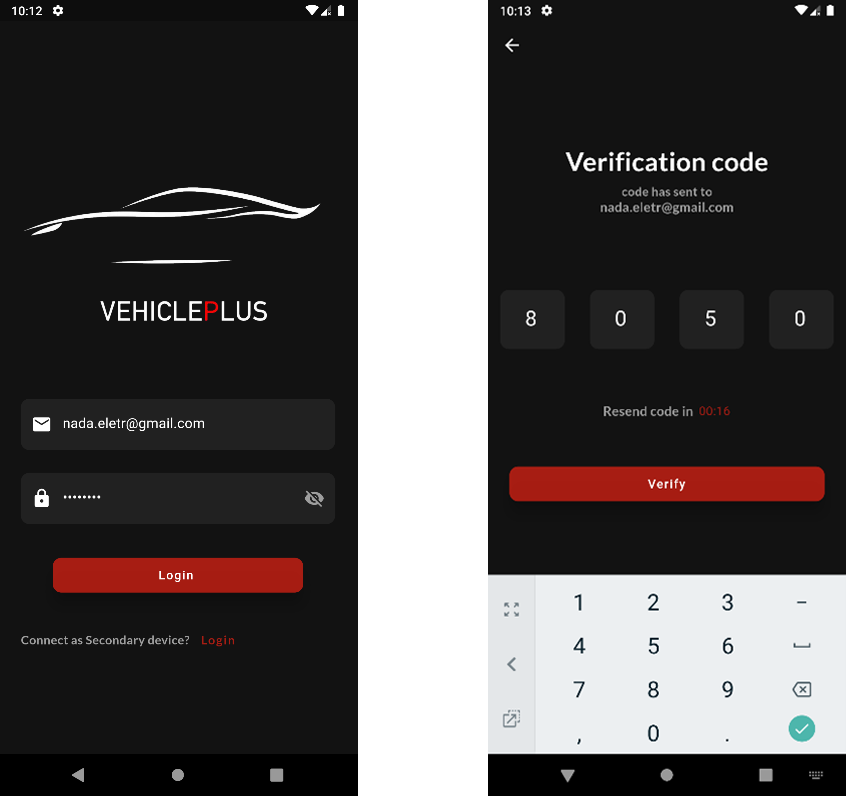
\includegraphics[scale=1]{Figures/mobileApp/1.png}
  	\caption{Mobile application primary login screens}
  	\label{fig:Mobile application primary login screens}
\end{figure}

\begin{enumerate}
\item Backend Implementation.
\begin{itemize}
\item The backend includes an endpoint "/authentication/mobile/login" that accepts a POST request from the Flutter mobile app to authenticate the user.
\item The backend verifies the user's credentials by using the UserManager provided by ASP.NET Core Identity.
\item If the credentials are correct, the backend generates a One-time password (OTP) and sends an email to the user's email account.
\item If the credentials are not correct, the server returns an appropriate error message to the mobile app.
\item The backend sends the email using the MailKit library, which is an open-source library for ASP.NET Core for handling mail tasks. It supports secure communication through the SSL/TLS protocol, ensuring a secure channel for communication.
\item Upon submitting the OTP code, the app sends a POST request to the "/authentication/mobile/verifymail" endpoint of the backend.
\item The request body includes the entered OTP code and user information in JSON format.
\item The backend verifies the OTP code by comparing it with the stored OTP in the database and checking its validity period.
\item If the OTP code is valid and within the expiration time, it responds with a JSON Web token (JWT) for subsequent requests.
\item If the OTP has expired or is invalid, the server returns an appropriate error message to the mobile app.
\end{itemize}
\end{enumerate}

\subsubsection{Sharing vehicle access through primary device}
The share access feature allows vehicle ownership to share access with other devices, whether it is sharing access with family member or granting temporary access to others. By generating a unique QR code on the primary device, users can easily share vehicle privileges with other devices. This eliminates the need for complex authentication processes and simplifies the sharing experience. With a simple scan of the QR code, secondary devices can establish a secure connection and gain access to shared vehicle features and functionalities.
\begin{enumerate}
\item Flutter Implementation.
\begin{itemize}
\item User initiates the process by sending a POST request to the server's "/authentication/mobile/shareAccess/request" endpoint along with the JSON Web token (JWT) in the authorization header.
\item The server receives the request and validates if the device is the primary device for the user.
\item If it is the primary device, the server generates a token along with the TCU ID and sends it back to the mobile app.
\item The mobile app directs the primary device to a generated QR code page.
\item When a secondary device wants to access the vehicle, it logs in as a secondary device.
\item The mobile app directs the user to a scanner page to scan the QR code displayed on the primary device.
\item After successful scanning, the secondary device makes a POST request to the server's "/authentication/mobile/shareAccess/submit" endpoint.
\item If the server verifies it, the secondary device is successfully connected to the vehicle and can access its functionalities.
\end{itemize}
\end{enumerate}

\begin{figure}[!ht]
	\centering
	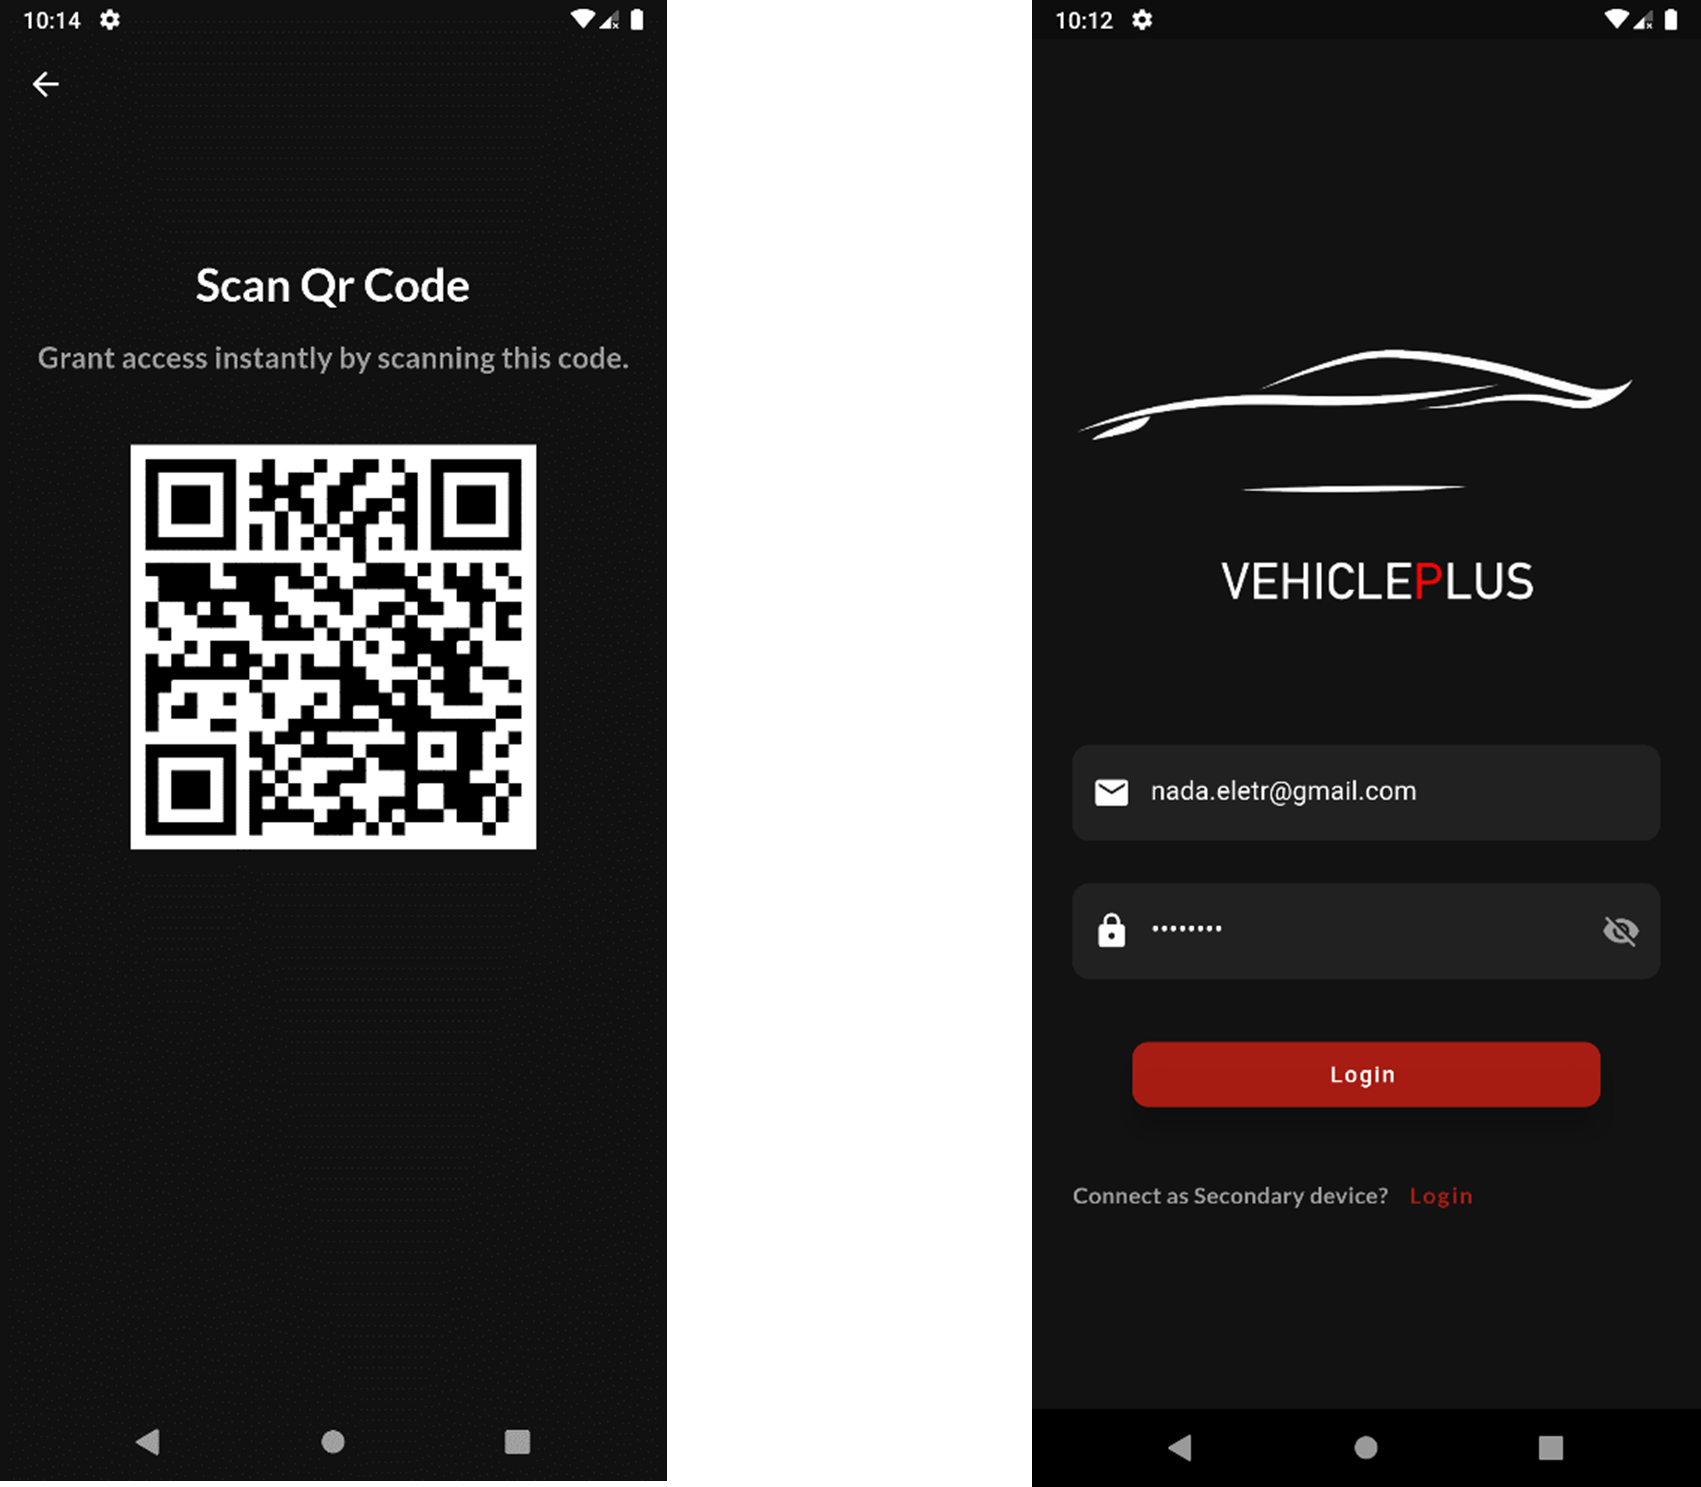
\includegraphics[scale=1]{Figures/mobileApp/2.png}
  	\caption{Mobile application sharing access screens}
  	\label{fig:Mobile application sharing access screens}
\end{figure}
\newpage
\begin{enumerate}
\item Backend Implementation:
\begin{itemize}
\item The request access:
\begin{itemize}
\item The backend includes an endpoint "/authentication/mobile/shareAccess/request" that accepts a POST request from the Flutter mobile app, requesting sharing access.
\item The backend server verifies the JSON Web token (JWT) and extracts the claims included in the authorization header.
\item After successful validation, a secure random token is generated, and a connection request record is created and stored in the database with the token, device ID, user ID, and the creation timestamp.
\item The token and TCU ID are returned as a response.
\end{itemize}
\item Submit Access Request:
\begin{itemize}
\item The backend includes an endpoint "/authentication/mobile/shareAccess/submit" that accepts a POST request from the Flutter mobile app.
\item The backend server extracts and verifies the token and TCU ID from the request body.
\item The server checks the expiration time of the connection request. If the connection request is valid, the server retrieves the user ID associated with the device used for the request.
\item If the request has expired, the server returns an appropriate error message to the mobile app.
\item A new Device record is created for the user, with the provided device ID, user ID, and IP address.
\item The device is connected to the vehicle, and a new JWT token is generated for the user.
\item The token, along with user details and expiration time, is returned as a response to the mobile app.
\end{itemize}
\end{itemize}
\end{enumerate}
\subsection{TCU authentication}
Implementing TCU (Telematics Control Unit) authentication in our project posed a significant challenge due to its unique requirements and criticality within the automotive domain. Unlike traditional authentication schemes, TCU authentication involves automatic identification and registration of vehicles without any user intervention. Moreover, the level of criticality associated with automotive authentication is considerably higher, as it directly impacts the security of a system considered a human safety critical system. To address these challenges, extensive research and a combination of multiple techniques were employed to provide robust and secure functionality.

One of the key aspects of TCU authentication is the automatic identification of vehicles. This involves implementing techniques such as digital certificates, secure protocols, and cryptographic algorithms to enable secure and automatic identification of vehicles. Digital certificates provide a means to establish the authenticity and trustworthiness of the vehicle, while secure protocols ensure the integrity and confidentiality of the communication between the TCU and the authentication system.

Additionally, a robust registration process had to be developed to facilitate automatic registration of vehicles on the system. This process involves securely exchanging and verifying vehicle credentials, such as vehicle identification numbers (VINs), manufacturer-specific data, and other unique identifiers. These credentials are used to authenticate the vehicle and establish a secure and trusted connection with the system.

To ensure the high level of criticality required for automotive authentication, multiple layers of security were implemented. This includes secure storage and handling of credentials, strong encryption algorithms, and strict access controls. Access to the authentication system is tightly regulated, with role-based access control and strict authentication policies in place to prevent unauthorized access and mitigate potential security threats.

Moreover, continuous monitoring and auditing mechanisms were incorporated into the authentication system to detect and respond to any potential security breaches or anomalies. This includes real-time monitoring of authentication requests, anomaly detection algorithms, and comprehensive logging and auditing of all authentication activities.

\subsubsection{vehicle registration}
The initial step in vehicle registration involves the generation of RSA public and private keys by the vehicle itself. This process takes place during the production line to ensure the integrity and security of the keys without any external system manipulation. The generated keys are then used to create a Certificate Signing Request (CSR) by the vehicle.

The CSR contains essential information about the vehicle, such as its identification details, and is submitted to the server for further processing. Upon receiving the CSR, the server utilizes the provided information to create a signed certificate. This certificate is then validated using the server's own certificate, establishing a certificate chain. The certificate chain ensures that the signed certificate can be verified using the server certificate, providing a trusted and secure means of identification.

Importantly, the chained certificate also incorporates the TCU hardware identifier, which typically includes the MAC address. This inclusion allows the certificate to possess the necessary credentials associated with the TCU. It is worth noting that these credentials are generated autonomously by the vehicle itself, with no way of predicting the specific public and private key pair. Additionally, throughout the entire registration process, the private key remains confidential and is never shared.

\begin{figure}[!ht]
	\centering
	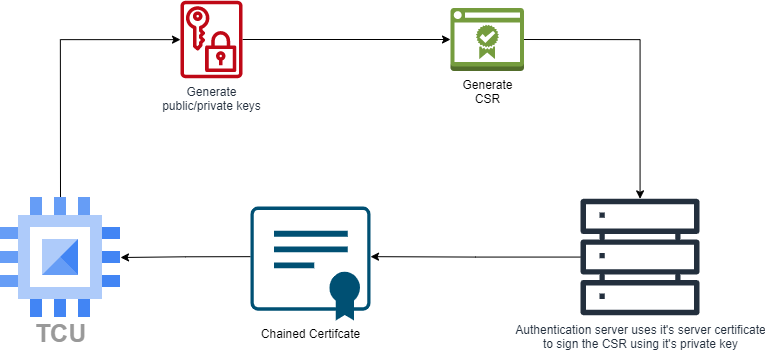
\includegraphics[scale=0.5]{Figures/Architicture/tcu_register.drawio.png}
  	\caption{TCU registration}
  	\label{fig:TCU registration}
\end{figure}

By following this approach, we establish a secure and reliable vehicle registration process. The generation of unique RSA key pairs and the subsequent creation of a signed certificate ensure the vehicle's identity and integrity. This method guarantees that each vehicle possesses a distinct certificate, making it uniquely identifiable within the system. This secure registration process reinforces the overall security of our cloud-based system, providing a robust foundation for subsequent authentication and communication between the TCU and the server.
\newpage
\subsubsection{Authentication using challenges}
To ensure secure authentication and log-in, our system incorporates challenge-based authentication in addition to validating the validity and ownership of the chained certificate. Challenge-based authentication adds an extra layer of security by requiring the entity to perform an action that only it has the capability to do, thus proving its authenticity.

\begin{figure}[!ht]
	\centering
	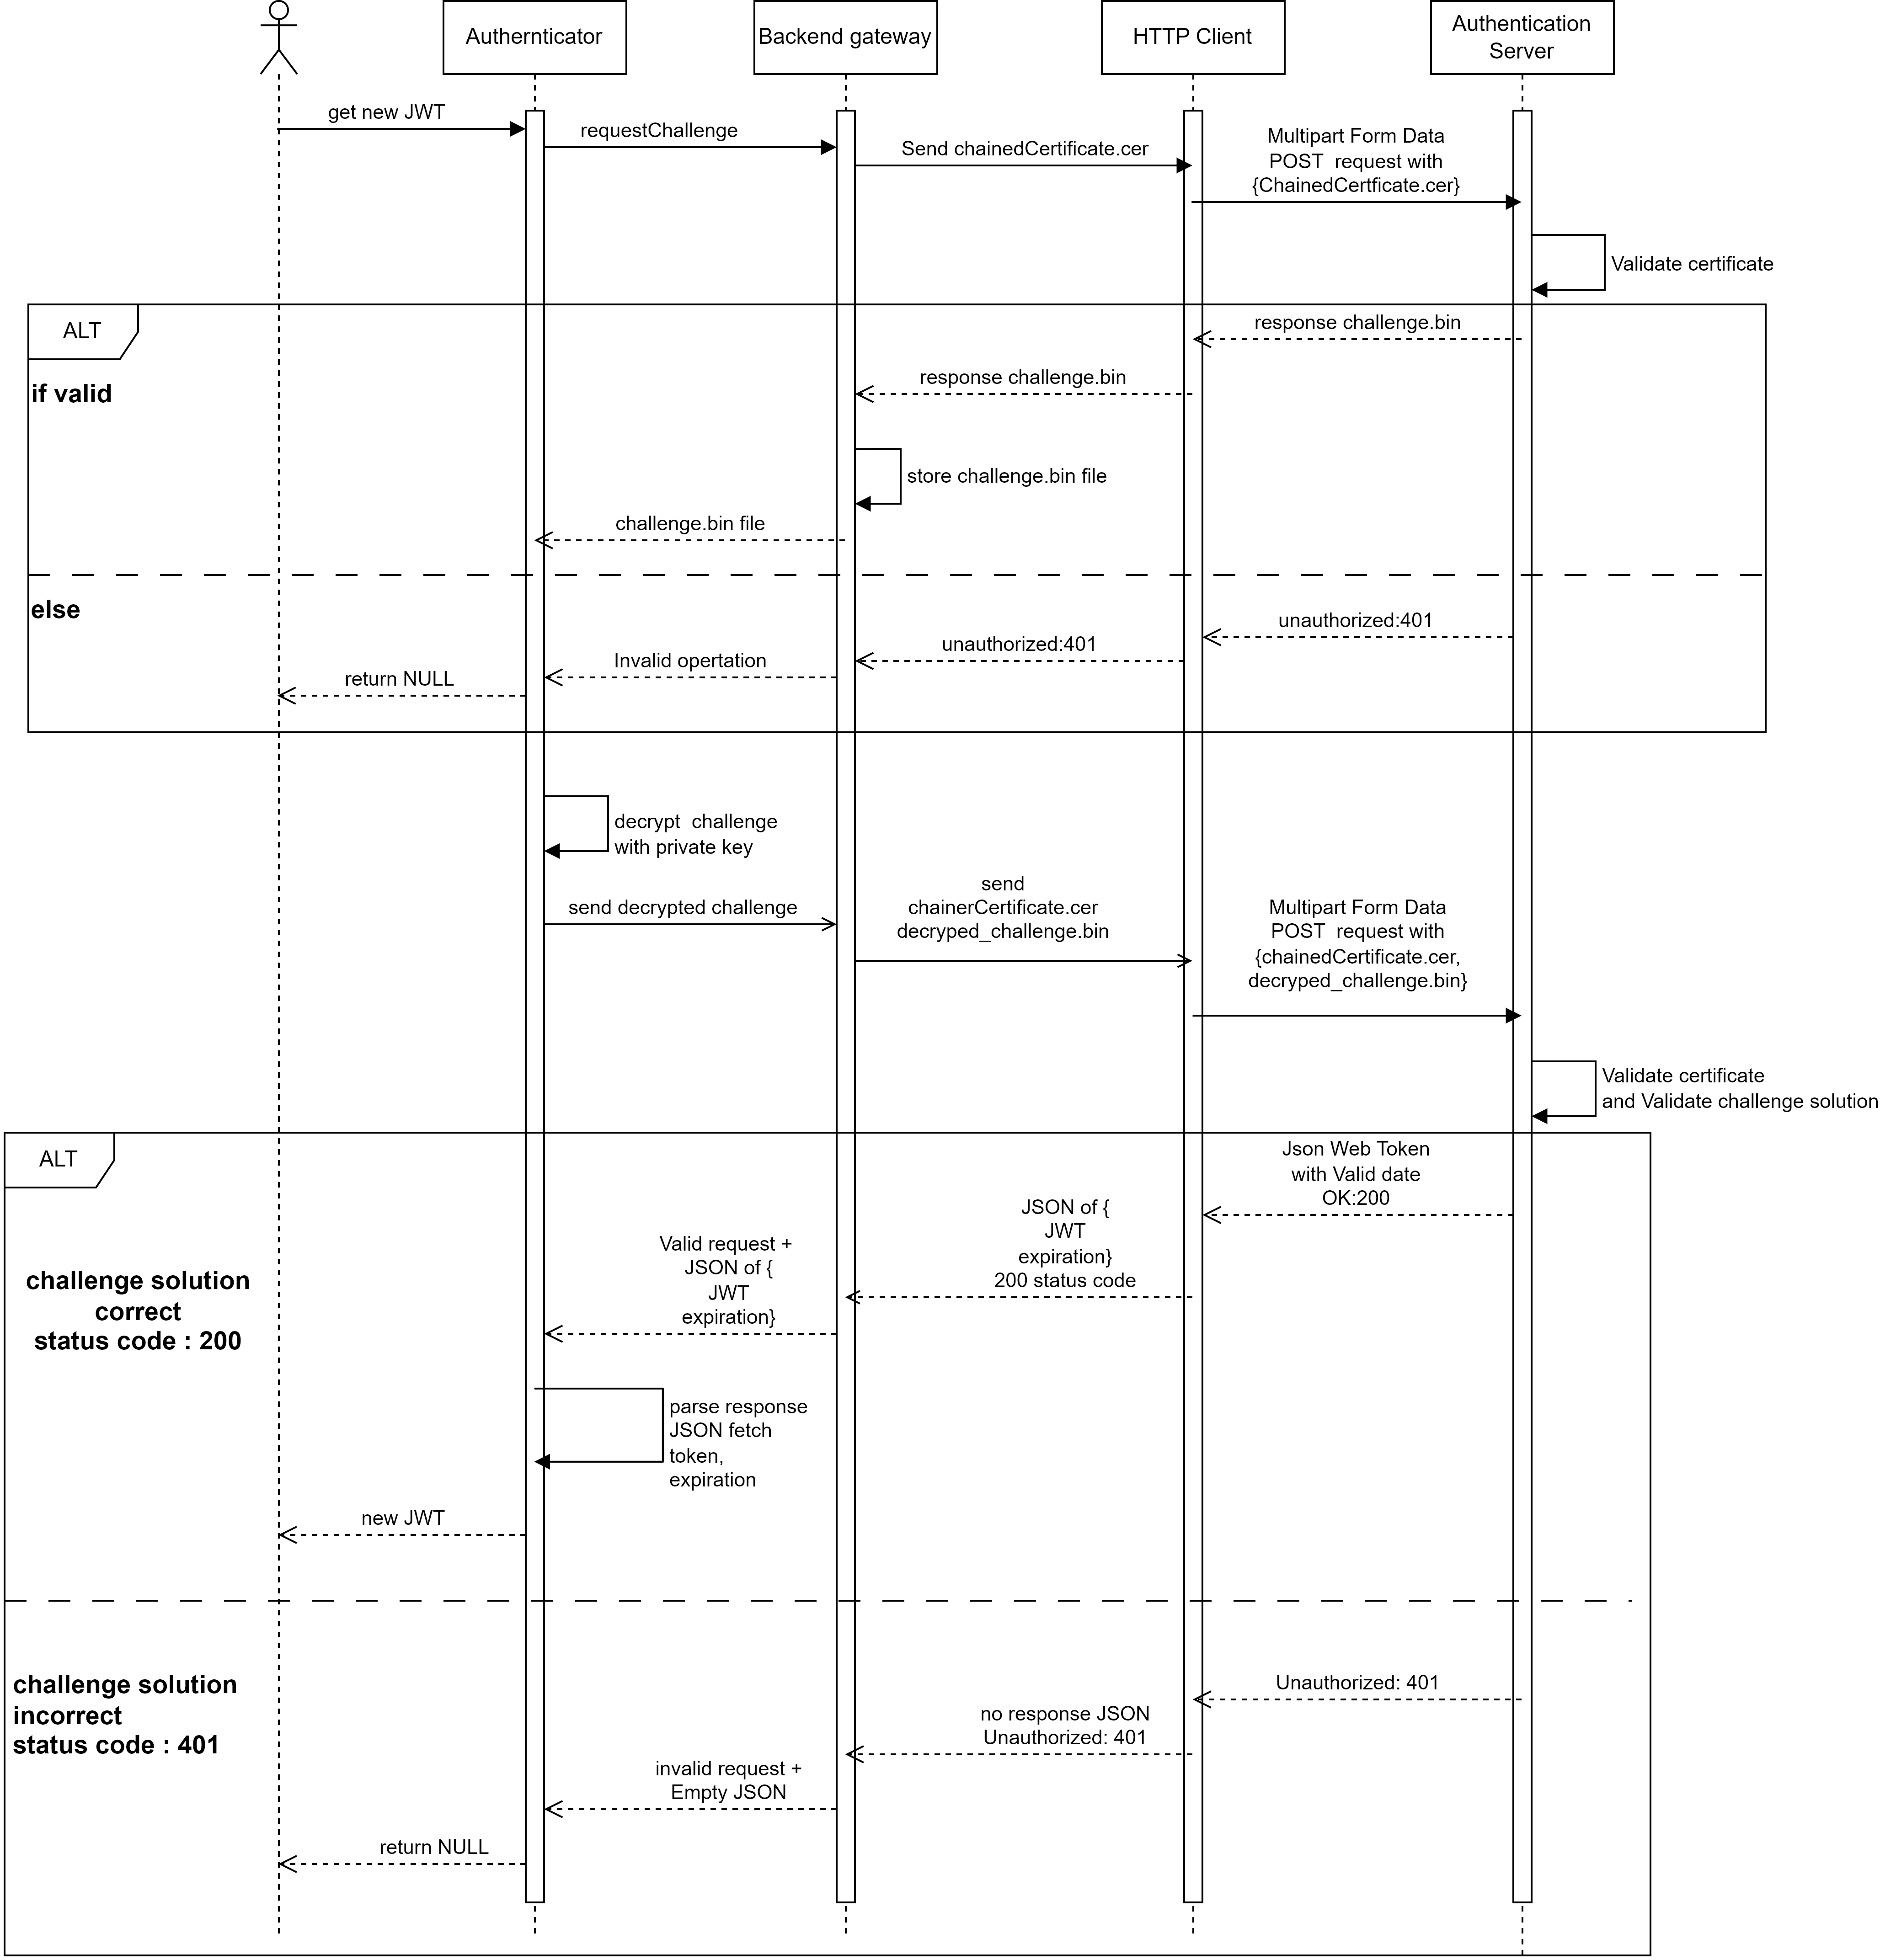
\includegraphics[scale=0.5]{Figures/Architicture/tcu_auth.png}
  	\caption{TCU login using challenge based authentication}
  	\label{fig:TCU login using challenge based authentication}
\end{figure}

In our solution, the TCU initiates the authentication process by requesting a challenge from the server. The challenge is a stream of bytes encrypted using the public key from the chained certificate, ensuring that only the corresponding private key held by the TCU can decrypt it. This challenge serves as a one-time passphrase that can be used for authentication.



Upon receiving the encrypted challenge, the TCU decrypts it using its private key, generating the one-time passphrase. This passphrase, combined with the chained certificate, is then used to initiate the login process on the server.

The server, upon receiving the login request, verifies the authenticity of the TCU by checking the MAC address embedded in the certificate. This MAC address serves as a unique identifier for the vehicle, confirming its identity and preventing unauthorized entities from accessing the server.



By employing challenge-based authentication, our system ensures that only the TCU possessing the private key linked to the public key used in generating the CSR can successfully decrypt the challenge and provide the corresponding passphrase. This approach provides a strong level of assurance in the authentication process and safeguards against unauthorized access to the server. The combination of chained certificates, MAC address verification, and challenge-based authentication establishes a robust and secure mechanism for TCU authentication within our cloud-based system.

\subsection{Token generation}
\begin{enumerate}
\item When a user successfully logs in, the backend server generates a JSON Web token (JWT) for authorization and authentication. The generation of the JWT involves the following steps:
\begin{enumerate}
\item Payload Construction: When generating the JWT, the server includes the necessary claims in the payload. In this case, the payload would include the device ID, user ID, and the claim "HasPrimaryDevice" indicating whether the user has a primary device.
\item Header Creation and Signing: The server creates the JWT header and signs the token using a secret key. The header would specify the token type (JWT) and the signing algorithm used.
\end{enumerate}
\end{enumerate}

Token Verification:
\begin{enumerate}
\item The verification of JWT involves the following steps:
\begin{enumerate}
\item Token Reception: Upon receiving a request with a JWT, the server extracts the token from the Authentication header in the request.
\item Token Decoding: The server decodes the base64-encoded header and payload sections of the JWT to access the claims, including the device ID, user ID, and "HasPrimaryDevice" claim.
\item Signature Verification: The server applies the same cryptographic algorithm and uses the secret key to recreate the digital signature from the header and payload sections.
\item Signature Comparison: The server compares the recreated signature to the signature contained in the received token. If they match, it is proof that the token has not been tampered with and is still authentic.
\item Claim Validation: The server checks the claims to ensure their validity.
\item User Authentication: If the token is correctly validated and the claims are true, the server provides the user access to the resources they have requested.
\end{enumerate}
\end{enumerate}

\section{Alerts and notifications}
The alert service in the mobile application plays a crucial role in keeping users informed about any malfunctions that occur in their vehicles. Its main objective is to send out notifications on time so that users are immediately informed of any potential problems. They can take appropriate measures, such as scheduling a maintenance appointment, contacting a service center, or performing necessary troubleshooting steps to address the malfunction promptly. When a malfunction is detected in the vehicle, it triggers a request to the back-end server, which in turn initiates the process of sending a notification to the user's mobile app.

\textbf{1- Firebase Cloud Messaging:}

Firebase Cloud Messaging (FCM) is an open-source cloud messaging service provided by Google that enables developers to send notifications and messages to mobile devices. It is a cloud-based service designed to handle the efficient delivery of messages. FCM supports multiple platforms, including IOS, Android, and web. Its purpose is to facilitate real-time communication between the back-end and mobile devices. FCM employs robust delivery mechanisms, including message handling, message queuing, and retries, ensuring reliable and efficient message delivery. In our project, FCM is used to send notification alerts to users when malfunctions occur in their vehicles.

\begin{figure}[!ht]
	\centering
	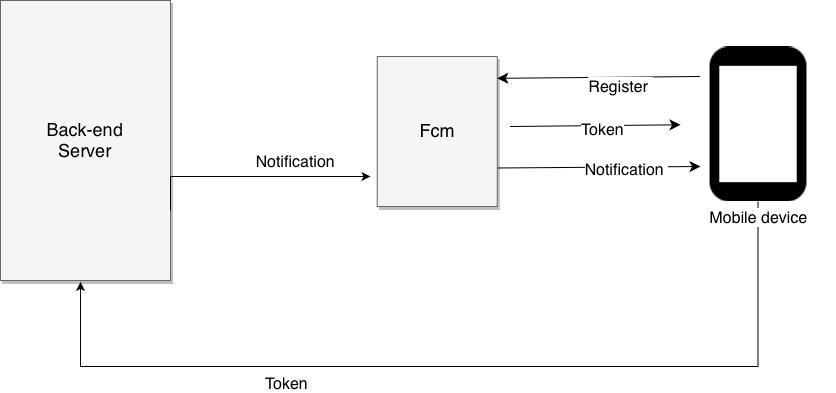
\includegraphics[scale=0.4]{Figures/Architicture/fcm.jpeg}
  	\caption{FCM architecture}
  	\label{fig:FCM architecture}
\end{figure}

\textbf{2- Flutter Implementation:}

\begin{itemize}
\item When a user first logs in, the mobile application registers on Firebase Cloud Messaging (FCM).
\item Upon successful registration, FCM generates a notification token for the device.
\item This token serves as a unique identifier for the device, enabling the backend server to send push notifications to the device.
\item The mobile application sends the generated FCM token to the backend server.
\item When the backend server needs to send a notification, it sends a notification request to FCM, specifying the target device using its notification token.
\item If the mobile application is in the foreground, the FCM service triggers a callback within the app, allowing it to handle and display the notification in real time.
\item If the mobile application is in the background or closed, FCM displays the notification directly to the device's notification system.
\end{itemize}

\begin{figure}[!ht]
	\centering
	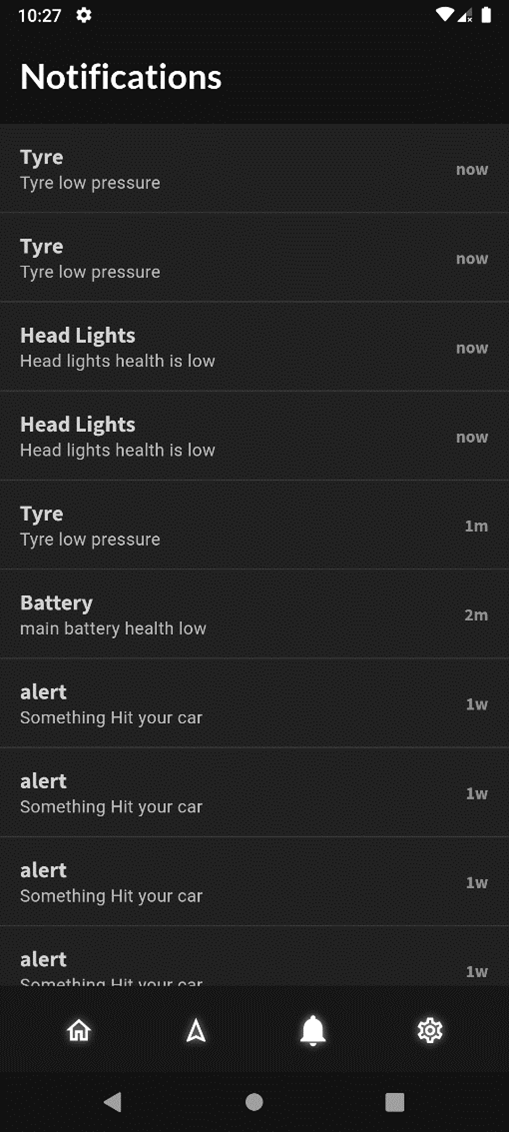
\includegraphics[scale=1]{Figures/mobileApp/3.png}
  	\caption{Mobile application Notifications screens}
  	\label{fig:Mobile application primary Notifications screens}
\end{figure}

\textbf{3- Backend Server Implementation:}

\begin{itemize}
\item When a malfunction occurs, the vehicle sends a request to the backend server's "alert/receive" endpoint.
\item The "alert/receive" endpoint is secured with the "TCUOnly" authorization policy, ensuring that only authorized TCU devices can access it.
\item The request payload should include the OBD code representing the specific vehicle malfunction.
\item The server validates the OBD code and ensures that it exists in the OBD codes database.
\item The alert is persisted in the database for further reference.
\item The server retrieves the list of devices associated with the TCU.
\item For each device, the server checks if a notification token is available.
\item If a notification token is found, the server uses the FCM service to send a notification with the alert details to the device.
\item The FCM service sends the notification using the notification token obtained from the device.
\end{itemize}

\section{Live location tracking}
Our vehicle tracking system is composed to two services that are integrated togther to provide the GPS live location functionality. Th first one is a SingalR server and the other is an MQTT client
\subsection{What is SingalR ?}
SignalR is a real-time communication library and framework developed by Microsoft for building interactive and responsive web applications. It simplifies the implementation of real-time functionality, enabling bidirectional communication between the server and the client. With SignalR, developers can create applications that deliver live updates, instant messaging, collaborative features, and real-time data streaming.

At its core, SignalR leverages various transport protocols, such as WebSockets, Server-Sent Events (SSE), and Long Polling, to establish a persistent connection between the server and the client. This connection allows the server to push updates and notifications to connected clients in real time, eliminating the need for traditional request-response patterns.

SignalR supports a wide range of platforms and programming languages, making it versatile and accessible. It provides client libraries for popular frameworks like JavaScript, .NET, and Java, enabling developers to integrate real-time functionality seamlessly into their applications regardless of the technology stack they are using.

One of the key advantages of SignalR is its automatic fallback mechanism. It gracefully handles scenarios where certain transport protocols are not supported by the client or the server, seamlessly falling back to an alternative transport method. This ensures wide compatibility and consistent real-time communication across different browsers and devices.

SignalR also offers features like group communication, allowing clients to be organized into groups and enabling targeted message delivery. It supports scaling out across multiple servers by leveraging technologies like Redis or Azure SignalR Service, ensuring high scalability and reliability for applications with a large number of concurrent connections.

Furthermore, SignalR provides a flexible and extensible programming model. Developers can define server-side hubs that expose methods and events, which can be invoked by clients or triggered by the server. This event-driven model simplifies the implementation of real-time functionality and enables easy integration with existing application logic.

Overall, SignalR empowers developers to create interactive and responsive web applications by facilitating real-time communication between the server and the client. Its simplicity, versatility, and support for various platforms make it a popular choice for applications that require live updates, collaborative features, and real-time data streaming.

\subsection{What does the MQTT client do ?}
In the implemented system, the MQTT client plays a crucial role in facilitating communication between the SignalR client and the vehicles. When the SignalR client needs to retrieve the GPS coordinates of a specific vehicle, it invokes the MQTT client to send a command to the respective vehicle. The command, encapsulated in a payload, includes the desired topic on which the vehicle should publish its GPS coordinates.

Upon receiving the command, the MQTT client establishes a connection with the MQTT broker and publishes the command payload to the designated topic. The vehicle, equipped with an MQTT client as well, is subscribed to the topic and upon receiving the command, it retrieves its GPS coordinates and publishes them on the specified topic.

The MQTT client, acting as a subscriber, ensures that it is subscribed to the relevant topic for receiving GPS coordinates from other vehicles. As vehicles publish their GPS coordinates on the corresponding topics, the MQTT client captures these updates and relays them back to the SignalR server.

By routing the GPS coordinates through the MQTT client and MQTT broker, the SignalR server can efficiently collect and distribute real-time vehicle location data to the connected SignalR clients. This enables the SignalR clients to display the live GPS coordinates of vehicles, visualize their positions on a map, or perform any other desired functionality based on the received location updates.

Overall, the integration of the MQTT client with the SignalR client and server facilitates the exchange of GPS coordinates between vehicles and the web application. The MQTT client handles the command invocation, publishing of commands to vehicles, subscription to GPS coordinate topics, and relaying of updates back to the SignalR server. This seamless communication enables real-time tracking and visualization of vehicle locations within the web application.

\subsection{System operation}
In the implemented system, when a user requests the GPS location of a vehicle, a WebSocket connection is established between the user's client and the SignalR server. The user's client then invokes a specific function on the SignalR server, requesting the vehicle's location. 

Upon receiving this request, the SignalR server utilizes the MQTT client to communicate with the MQTT broker. The MQTT client sends a request to the vehicle, instructing it to provide its GPS location. The request is sent using a topic that is specifically mapped to the user's connection ID, ensuring that the location data is streamed back to the correct user.

The Telematics Control Unit (TCU) in the vehicle is connected to the MQTT broker and actively subscribes to the server's client call topic. When it receives the request for its GPS location, the TCU retrieves the location information and publishes it on the designated MQTT topic.

The MQTT broker then forwards the published GPS location to the SignalR server. Upon receiving this data, the SignalR server identifies the corresponding user connection ID and invokes the appropriate function to send the location back to the user's client.

By utilizing a combination of SignalR, MQTT, and WebSocket connections, this system enables real-time communication between the user, the SignalR server, the MQTT client, and the Telematics Control Unit. It allows the user to request and receive the GPS location of a specific vehicle, with the MQTT broker and SignalR server facilitating the seamless exchange of data between all parties involved.

\chapter{TCU integration}
\section{vehicle signaling}
To ensure efficient and secure vehicle signaling, we have implemented a comprehensive software stack consisting of two key components: an MQTT broker and an authentication and authorization server. This software stack forms the backbone of our signaling system, facilitating seamless communication and enforcing access control measures.


\begin{figure}[!ht]
	\centering
	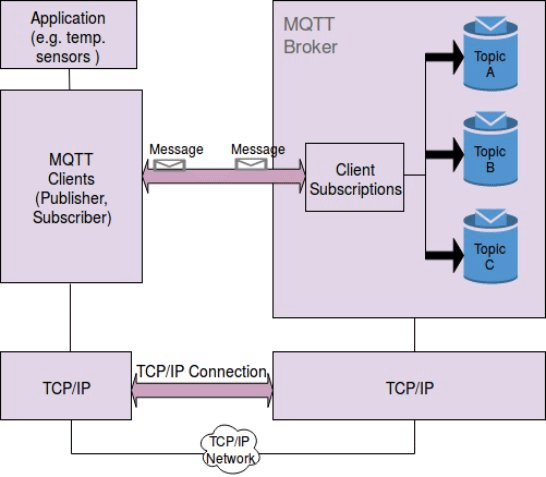
\includegraphics[scale=0.5]{Figures/Architicture/mqtt.png}
  	\caption{MQTT architecture}
  	\label{fig:MQTT architecture}
\end{figure}


The MQTT broker serves as the central messaging hub, responsible for receiving and distributing messages between vehicles and other connected devices. It provides a lightweight and scalable publish-subscribe messaging protocol that enables efficient and real-time communication. By utilizing the MQTT protocol, we ensure reliable and low-latency data exchange, essential for time-sensitive signaling in the automotive domain.

In addition to message routing, the MQTT broker also plays a critical role in enforcing access control and maintaining accountability. It acts as the gatekeeper, ensuring that only authorized devices and users can participate in the communication network. This prevents unauthorized access and potential security breaches within the system. By hosting the MQTT broker as part of our software stack, we can establish granular access control policies, restricting communication to authorized vehicles and authenticated users.

To manage authentication and authorization, we have integrated an authentication and authorization server with the MQTT broker. This server acts as a centralized authority responsible for validating the identities of vehicles and users, ensuring that only trusted entities can access the signaling system. It employs robust authentication mechanisms, such as username-password authentication or certificate-based authentication, to verify the credentials provided by vehicles and users.

Furthermore, the authentication and authorization server handles the enforcement of access control policies. It determines the privileges and permissions granted to each vehicle or user, allowing fine-grained control over the topics they can publish to or subscribe to within the MQTT broker. By implementing such access control mechanisms, we can ensure that sensitive information is only accessible to authorized entities, enhancing the security and integrity of the signaling system.

\subsection{MQTT broker}
For our MQTT broker, we have made the decision to host an EMQ X server, which is widely recognized as an enterprise-grade solution and has been adopted by several leading OEMs, including Volkswagen. The MQTT broker serves as a crucial component of our signaling system, providing a comprehensive set of features that enable efficient and secure communication between devices.

One of the primary advantages of utilizing the EMQ X server is its support for publishing and subscription using topics. This topic-based communication mechanism allows for a flexible and scalable approach to routing messages within the system. By subscribing to relevant topics, devices can receive only the information they are interested in, overcoming the challenge of determining the logical address of each individual vehicle. This efficient topic-based messaging simplifies the overall communication architecture and enhances the scalability of our system.



In terms of security, the EMQ X server offers a robust solution by providing a secure SSL encrypted tunnel for vehicle communication. This ensures that all data transmitted between the vehicles and the server is encrypted, preventing unauthorized access and tampering. The SSL encryption guarantees the confidentiality and integrity of the communication, safeguarding sensitive information exchanged within the system.

Another important aspect of the MQTT broker is its support for different levels of Quality of Service (QoS), which determine the reliability of message delivery. The EMQ X server offers configurable QoS levels, allowing us to choose the appropriate level based on the requirements of each message. This flexibility enables us to strike a balance between reliable message delivery and system performance, ensuring that critical messages are reliably delivered while optimizing network resources.

Furthermore, the MQTT broker includes the capability of message retaining. When a client is offline or disconnected temporarily, the EMQ X server retains the messages intended for that client in a queue. Once the client reconnects, it receives all the messages that were retained, ensuring that no information is lost during periods of disconnection. This feature is particularly valuable in scenarios where real-time data updates are crucial, as it ensures that clients are always up-to-date with the latest information.
\subsection{Customized authentication and authorization}
To manage authentication and access control, we have developed a custom authentication server using ASP.NET Core API. This authentication server acts as a central authority for validating user credentials and determining their access privileges within the system. It enables fine-grained control over user permissions, allowing us to specify the topics that each user is permitted to publish on or subscribe to. This granular access control ensures that only authorized users can participate in the communication system and interact with specific topics, enhancing the overall security of our infrastructure.

In summary, the selection of the EMQX server as our MQTT broker, combined with the implementation of a custom authentication server, provides a robust and secure foundation for our signaling system. The EMQ X server's support for topic-based communication, SSL encryption, configurable QoS levels, and message retaining ensures efficient, reliable, and secure communication between devices. By integrating these components, we have created a resilient and scalable infrastructure that meets the high standards required in the automotive industry, ensuring the privacy, integrity, and availability of our communication system.
\section{Customization using OTA updates}
To enable feature customization for vehicles, a System Update Management System (SUMS) was implemented as part of the infrastructure. The SUMS system consists of several key components that facilitate the distribution and installation of software features.

The first component is a container registry, which serves as a centralized repository for developers to upload their software as container images. To ensure security and authorization, a private repository was created and hosted on the server. This private repository ensures that only authorized and verified software images are available for distribution.

To track changes and updates in the container registry, a system was implemented to listen for events through webhooks. Whenever a change occurs in the registry, such as a new feature or an updated version, the system is notified. This ensures that any changes or updates are promptly captured and logged for further processing.

Each change or update in the container registry is logged by the system by updating that feature record on the database. This logging mechanism provides a comprehensive history of all changes, allowing for easy tracking and reference.


Then this feature is published as an application through the admin console application as a feature where all the data required for that feature configuration including the release time.

 \begin{figure}[!ht]
	\centering
	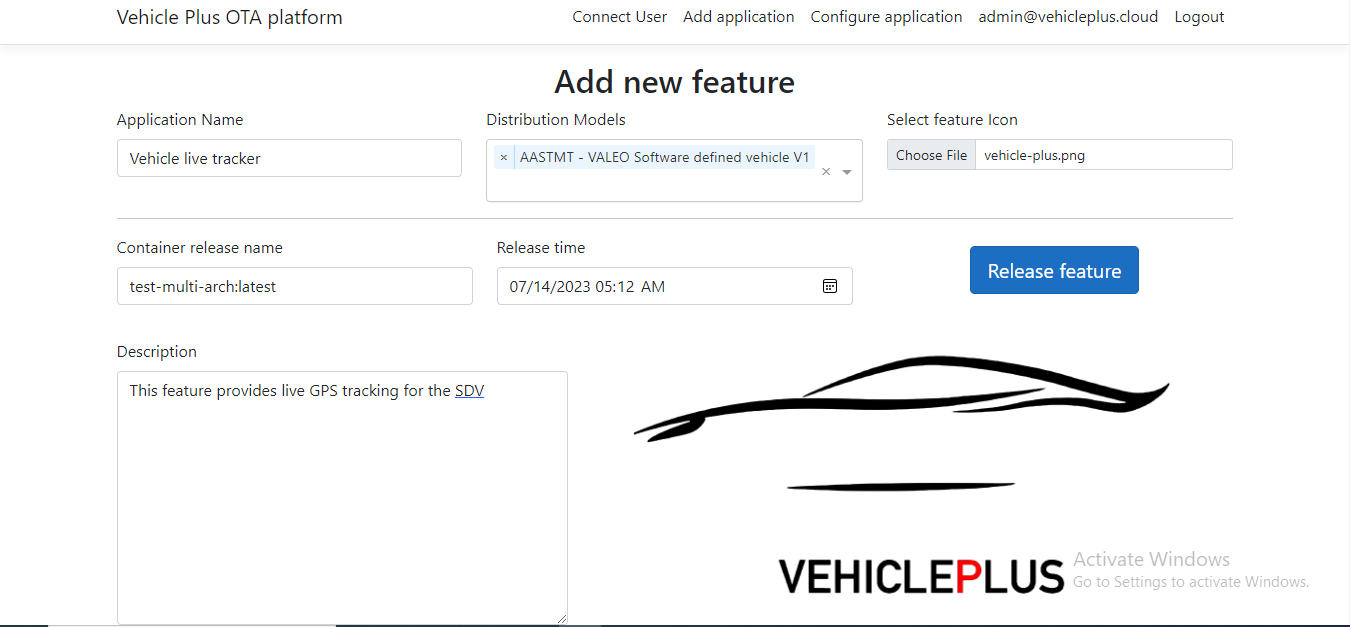
\includegraphics[scale=0.4]{Figures/FrontEnd/AdminConsole/add.PNG}
  	\caption{Admin console add feature screen}
  	\label{fig:Admin console add feature screen}
\end{figure}

 \begin{figure}[!ht]
	\centering
	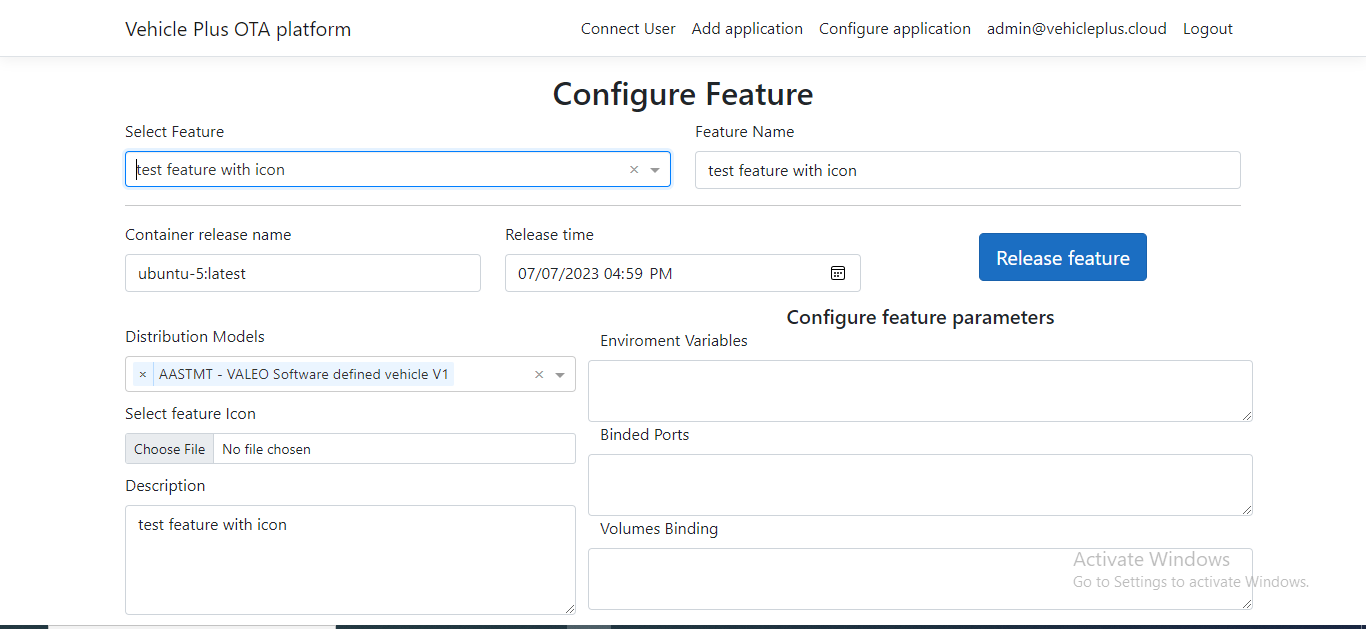
\includegraphics[scale=0.4]{Figures/FrontEnd/AdminConsole/configure.PNG}
  	\caption{Admin console configure feature screen}
  	\label{fig:Admin console configure feature screen}
\end{figure}

On release time, to notify users about the availability of new features or updates, the system utilizes FCM (Firebase Cloud Messaging) notifications. Users are promptly informed via these notifications, ensuring they are aware of the latest additions or improvements to the available features.

When a user expresses their interest in installing a specific feature, the system receives the notification and initiates the installation process.

 \begin{figure}[!ht]
	\centering
	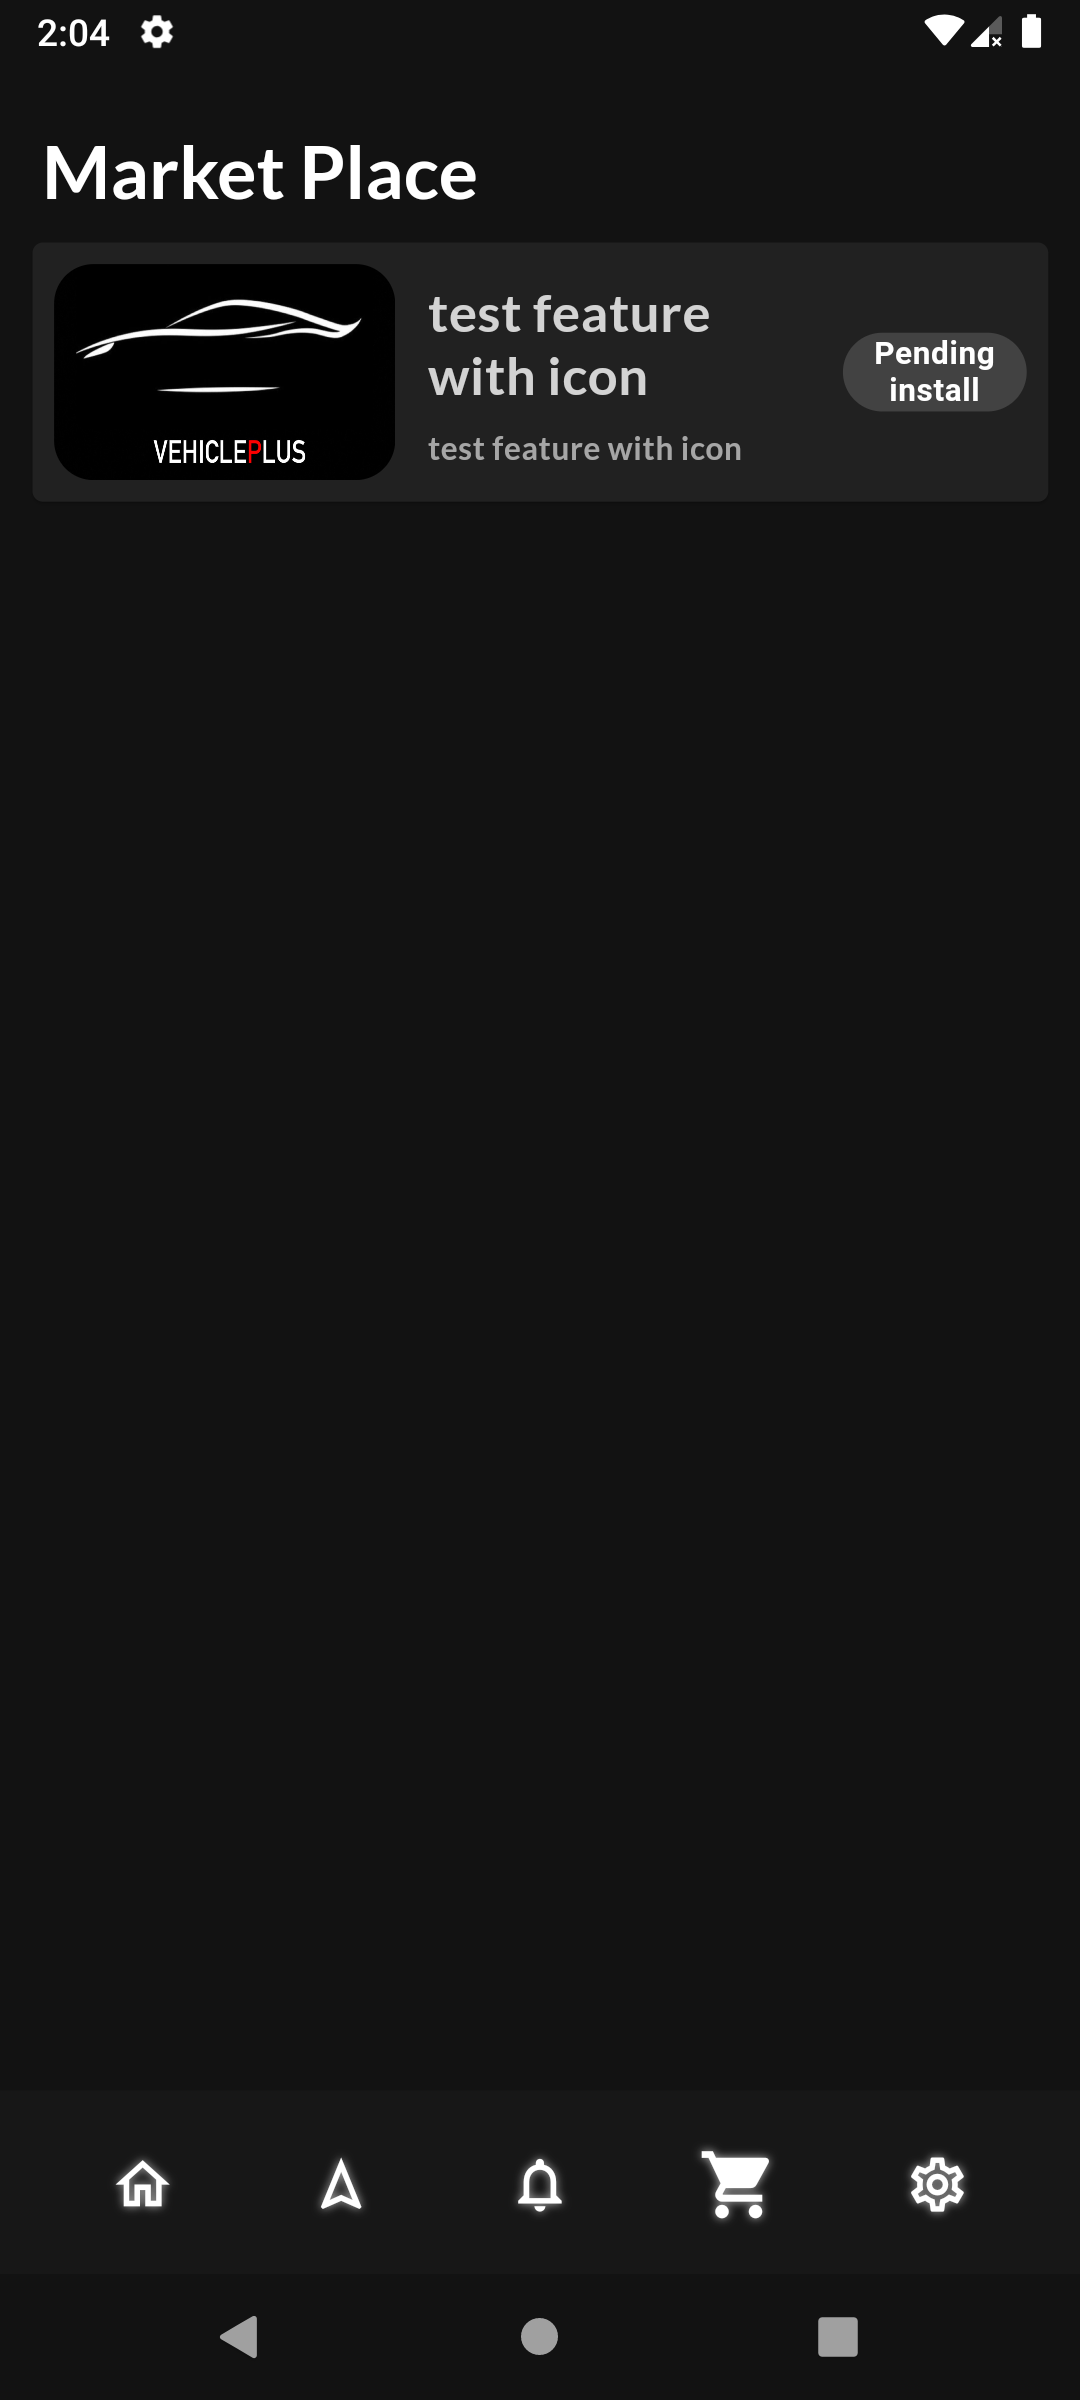
\includegraphics[scale=0.15]{Figures/mobileApp/5.png}
  	\caption{Mobile market place screen}
  	\label{fig:Mobile market place screen}
\end{figure}

On the next vehicle wake up the vehicle will request updates and then installs them.

To ensure the integrity of the downloaded container images, they are downloaded as context blocks, and each block is associated with an SHA256 hash checksum. This checksum verification process guarantees that the downloaded image has been received without any corruption or tampering, providing an added layer of security and reliability.

The implementation of the SUMS system offers a robust and secure mechanism for distributing and installing software features in vehicles. It combines containerization technology, container registry management, change tracking, notification systems, and secure image downloading to enable efficient and customizable feature deployment. This approach aligns with industry best practices and ensures a professional and reliable feature customization process for vehicle owners.

\chapter{Conclusion and future work}
\section{Conclusion}
In conclusion, software-defined vehicles represent a transformative leap forward in the automotive industry, offering a multitude of benefits that can revolutionize the way we conceive, manufacture, and experience vehicles. By decoupling hardware from software, these vehicles bring increased flexibility, scalability, and customization possibilities for manufacturers and consumers alike.

One of the primary advantages of software-defined vehicles is the streamlined production process they enable. Manufacturers can focus on developing standardized hardware components that can be utilized across different vehicle models. This approach simplifies manufacturing, reduces costs, and accelerates production cycles. Additionally, remote software updates and customizations can be seamlessly applied without the need for physical modifications, further enhancing efficiency and reducing time-to-market.

From a consumer perspective, software-defined vehicles offer an enhanced driving experience. Through over-the-air updates, these vehicles can continuously receive the latest software upgrades, bug fixes, and feature enhancements. This ensures that the vehicle's performance, safety features, and infotainment systems remain up to date throughout its lifespan. Moreover, software-defined vehicles allow for personalized settings and preferences, tailoring the driving experience to individual users' preferences and needs.

The integration of software-defined vehicles with the cloud takes these benefits to a new level. By leveraging the power of cloud computing resources, manufacturers gain access to massive computational capabilities and storage capacities. This empowers vehicles with advanced technologies such as artificial intelligence, machine learning, and predictive analytics. Real-time data processing, analysis, and decision-making become possible, enabling vehicles to make intelligent, data-driven decisions on the road. Furthermore, seamless connectivity facilitated by the cloud allows vehicles to communicate with each other, infrastructure, and other devices, leading to improved safety, efficient traffic management, and the development of autonomous driving capabilities.

Another significant advantage of cloud integration is the ability to collect and analyze vast amounts of data generated by software-defined vehicles. This data can provide valuable insights into vehicle performance, usage patterns, and user behavior. Manufacturers can leverage this information to improve their products, optimize maintenance schedules, and develop new services tailored to customer needs. The cloud platform becomes a powerful tool for innovation and continuous improvement in the automotive industry.

However, it is crucial to address the challenges and concerns associated with software-defined vehicles and cloud integration. Security and privacy become paramount considerations when dealing with connected vehicles and sensitive user data. Robust cybersecurity measures and data protection protocols must be implemented to safeguard against unauthorized access and ensure the privacy of users' information.

In summary, the integration of software-defined vehicles with cloud technology presents an exciting opportunity for the automotive industry. By embracing this innovative approach, manufacturers can achieve streamlined production processes, personalized driving experiences, and access to advanced computational capabilities. Cloud integration enables the collection and analysis of valuable data, empowering manufacturers to optimize their products and services. While challenges exist, addressing them through robust security measures can ensure a safer and more connected future for software-defined vehicles. By embracing the potential of software-defined vehicles and cloud integration, we can drive the industry forward and shape the future of mobility.

\section{Future Work}
\subsection{Cloud native Testing}
Modern DevOps processes have robust testing infrastructure build into their testing and deployment pipelines. Currently this infrastructure from the cloud-native world lacks the ability to test and validate real-time workloads, or workloads that are targeting real-time or microcontroller based architectures. We need to enhance the cloud based tooling to meet the validation needs of safety and real-time domains.
\subsection{Cloud Native Trail}
The adoption of Cloud Native in Automotive requires collaboration and contribution of many different stakeholders. To indicate a clear and stepwise approach for a migration, a clear trail needs to be described 

%----------------------------------------------------------------------------------------
%	REFERENCES TABLE (DO NOT MODIFY)
%----------------------------------------------------------------------------------------
\newpage
\phantomsection 
\addchaptertocentry{References}  
\begin{center}{\Large\MakeUppercase{\textbf{References}}\par}\end{center}
\vspace{20pt}
\printbibliography[heading=none]

%----------------------------------------------------------------------------------------
%	APPENDICES START HERE (MODIFY AS DESIRED)
%----------------------------------------------------------------------------------------
\appendixstart 
\chapter{RSA algorithm}
Certainly! Here's a paragraph about the RSA algorithm with equations:

The RSA algorithm, named after its inventors Rivest, Shamir, and Adleman, is a widely used public-key encryption system that relies on the computational difficulty of factoring large prime numbers. The algorithm utilizes modular exponentiation and number theory principles to achieve secure encryption and decryption. Let's denote the public key as (e, N), where e is the encryption exponent and N is the modulus, and the private key as (d, N), where d is the decryption exponent and N is the same modulus. The encryption process involves raising the plaintext message, denoted as M, to the power of e and taking the remainder when divided by N. This yields the ciphertext C:

$C = M^{e} MOD N$

To decrypt the ciphertext C back to the original plaintext M, the recipient uses their private key exponent d and applies the following formula:

$M = C^{d} MOD N$

The security of RSA rests on the difficulty of factoring the modulus N into its prime factors. Breaking RSA encryption requires determining the values of d and N from the public key information, which is computationally infeasible when N is a large semiprime number. The larger the prime factors and the modulus, the more secure the RSA encryption becomes. The RSA algorithm's versatility and robustness have made it a cornerstone in modern cryptography, ensuring secure data transmission and encryption in various domains.

\chapter{Digital Certificates}
Digital certificates are electronic documents that bind cryptographic keys to the identity of an entity, such as an individual, organization, or device. They play a crucial role in ensuring secure communication and authentication in various digital applications. Different types of digital certificates serve specific purposes and provide different levels of trust and security. Here are some common types of digital certificates:
\section{X.509 Certificates}
1. X.509 Certificates: X.509 is the most widely used standard for digital certificates. These certificates contain information about the certificate holder, including their public key, name, and other relevant details. X.509 certificates are commonly used in secure communication protocols such as SSL/TLS for secure websites, S/MIME for email encryption, and IPsec for virtual private networks (VPNs).
\section{SSL/TLS Certificates}
SSL (Secure Sockets Layer) and its successor TLS (Transport Layer Security) utilize X.509 certificates to establish secure connections between web servers and clients. SSL/TLS certificates verify the authenticity of the server and enable encrypted communication, protecting sensitive data during online transactions, login processes, and other interactions over the internet.
\section{Code Signing Certificates}
Code signing certificates are used by software developers to digitally sign their applications and software updates. These certificates ensure that the code has not been tampered with during distribution, providing users with assurance of the software's authenticity and integrity. Code signing certificates are commonly used in platforms such as Windows, macOS, and mobile app stores.
\section{Client Certificates}
Client certificates, also known as personal certificates or user certificates, are issued to individuals for authentication purposes. These certificates are used in scenarios where the server requires verification of the client's identity. For example, client certificates are employed in secure email systems, virtual private networks (VPNs), and other applications where strong user authentication is essential.
\section{Extended Validation (EV) Certificates}
EV certificates are a specific type of X.509 certificate that provides the highest level of assurance and trust for websites. They involve a rigorous validation process to verify the legal and operational existence of the entity behind the website. EV certificates trigger the display of a green address bar in web browsers, indicating to users that they are visiting a highly authenticated and secure website.
\section{Self-Signed Certificates}
Self-signed certificates are generated by individuals or organizations themselves, without involving a trusted third-party Certificate Authority (CA). These certificates are mainly used for internal testing, development environments, or private networks. While self-signed certificates can provide encryption, they lack the trusted validation of CA-issued certificates, resulting in security warnings in web browsers.

It is important to note that digital certificates rely on the trust and integrity of Certificate Authorities (CAs) that issue and validate them. CAs play a critical role in verifying the identity of certificate applicants and signing the certificates, thereby establishing trust in the digital ecosystem. Choosing the appropriate type of certificate depends on the specific use case and the level of trust and security required.
%----------------------------------------------------------------------------------------
%	ARABIC ABSTRACT (MODIFY AS DESIRED)
%----------------------------------------------------------------------------------------
\begin{arabicabstractp}
\begin{Arabic}
تكنولوجيا المركبات ذات البرمجة البرمجية قد ظهرت كتقنية مبتكرة في صناعة السيارات، مما جذب اهتمام الشركات المصنعة الأصلية واللاعبين الرئيسيين في هذا المجال. تهدف هذه الرسالة إلى استكشاف إمكانات sVDS من خلال تحقيق عدة أهداف.

الهدف الأول هو إنشاء منصة سحابية متكاملة مع وحدات التحكم التلماتكية، والتي تمكِّن تحويل المركبات إلى كيانات محددة بالبرمجيات. تتيح هذه المنصة التحديثات القياسية والمستقلة والآمنة لنظام المركبة، بنفس طريقة تعديل إعدادات الهاتف المحمول. بالإضافة إلى ذلك، يتم تطوير نظام إدارة تحديث البرمجيات لتتبع وتوجيه عمليات التحقق والاختبار والنشر لهذه التحديثات من خلال واجهة المسؤول.

الهدف الثاني يركز على تأمين اتصال المركبة إلى المركبة )V2V( باستخدام تكنولوجيا اتصال المركبة إلى البنية التحتية )I2V(. يتم اقتراح بنية تحتية تسمح للمركبات بتسجيل أنفسها في مناطق جغرافية، مما يتيح للمركبات الأخرى تحديد هويتها وضمان صحة المركبات المحيطة. يتحسن الأمان العام ويتيح الاتصال الآمن والموثوق به للمركبات إلى المركبات.

علاوة على ذلك، تستكشف هذه الرسالة تطوير واجهة بديهية لأصحاب السيارات للوصول إلى مركباتهم من هواتفهم الذكية. تتيح هذه الواجهة التحكم المريح ومراقبة وظائف المركبة، مما يعزز تجربة المستخدم والراحة.

بالإضافة إلى ذ

لك، يتم تقديم ميزات الاتصال بالسحابة للمركبة إلى السحابة)C2V(، مما يوفر للمركبات القدرة على الاتصال والتواصل مع خدمات قائمة على السحابة. يتيح هذا للمركبات الوصول إلى مجموعة واسعة من الخدمات والبيانات، مثل معلومات حركة المرور في الوقت الحقيقي، وتحديثات البرامج، والإعدادات الشخصية. يعزز الاتصال C2V الوظائف والقدرات لـsVDS، مما يحسن راحة المستخدم ويوسع مجال الخدمات المتاحة.

لاعبون رئيسيون في الصناعة، بما في ذلك تيسلا، WMB، omyaW، MG،AIDIVN، و oelaV، قد أبدوا اهتمامًا واستثمارًا كبيرًا في sVDS. تعترف هذه الشركات بإمكانات sVDS للتمييز بمنتجاتها، وإدخال ميزات مبتكرة، وتبسيط عمليات الإنتاج. تشير مشاركتهم إلى أهمية البرمجيات والاتصالات المتزايدة في صناعة السيارات.

بشكل عام، تسهم هذه الرسالة في تقدم sVDS من خلال تحقيق أهداف رئيسية، واستكشاف الفوائد المحتملة، وإبراز الاهتمام والمشاركة من قبل الشركات الرائدة في الصناعة. تمهد النتائج الطريق لمزيد من البحث والتطوير في مجال المركبات ذات البرمجة البرمجية المثير.
\end{Arabic}
\end{arabicabstractp}

\end{document}  
